\chapter{Realisation Phase}
The realisation phase, is where all the analysis, design, implementation, verification and deployments is made. This phase is divided into several timeboxes, where small parts of the development is done in steps. A timebox is a 2 week time period where parts of the product is made ready for deployments for the end product.
\p The work that shall be done to complete the project is stated below:\p
\textbf{System setup / Design:}\\
CO/Module-design. Deadline in week 10\\
Relay server. Deadline tuesday week 9\\
Daemon. Deadline week 11\\
Almost complete system. Deadline week 13\\
Complete system. Deadline week 15\\
\\
\textbf{Hardware:}\\
\textit{ARM7 / FPGA connector}\\
- Schematic\\
- Print layout\\
- Mounting\p
\textit{PLC module + 5v supply (Dennis responsible with Kristian). Deadline week 9}\\
- Schematic\\
- Print layout\\
- Mounting\\
- Functional test\\
- EMC test\p
\textit{Power switch:}\\
	- Block diagram with state machine\\
	- Schematic\\
	- Simulation\\
	- Print layout\\
	- Mounting\\
	- Testing\p
\textit{FPGA extension board}\\
- Schematic (Temp + humidity circuit + current sensor circuit)\\
- Print layout\\
- Mounting\\
- Functional test\p
\textit{Converters}\\
- 230VAC - 30VDC inverter\\
- 30VDC - 230VAC converter\\
- Possible Variable load.\\\p
\textbf{Mechanic:}\\
Box for the hub\p
\textbf{Software:}\\
Web application - Database and server side programming\\
ADC\\
Daemons\\
Drivers\\

%\section{Project time plan}
\section{Time box 1}
\subsection{Time box planning}
Overview of the what work is putted into which time boxes.
\begin{figure}[H]
	\begin{centering}
		 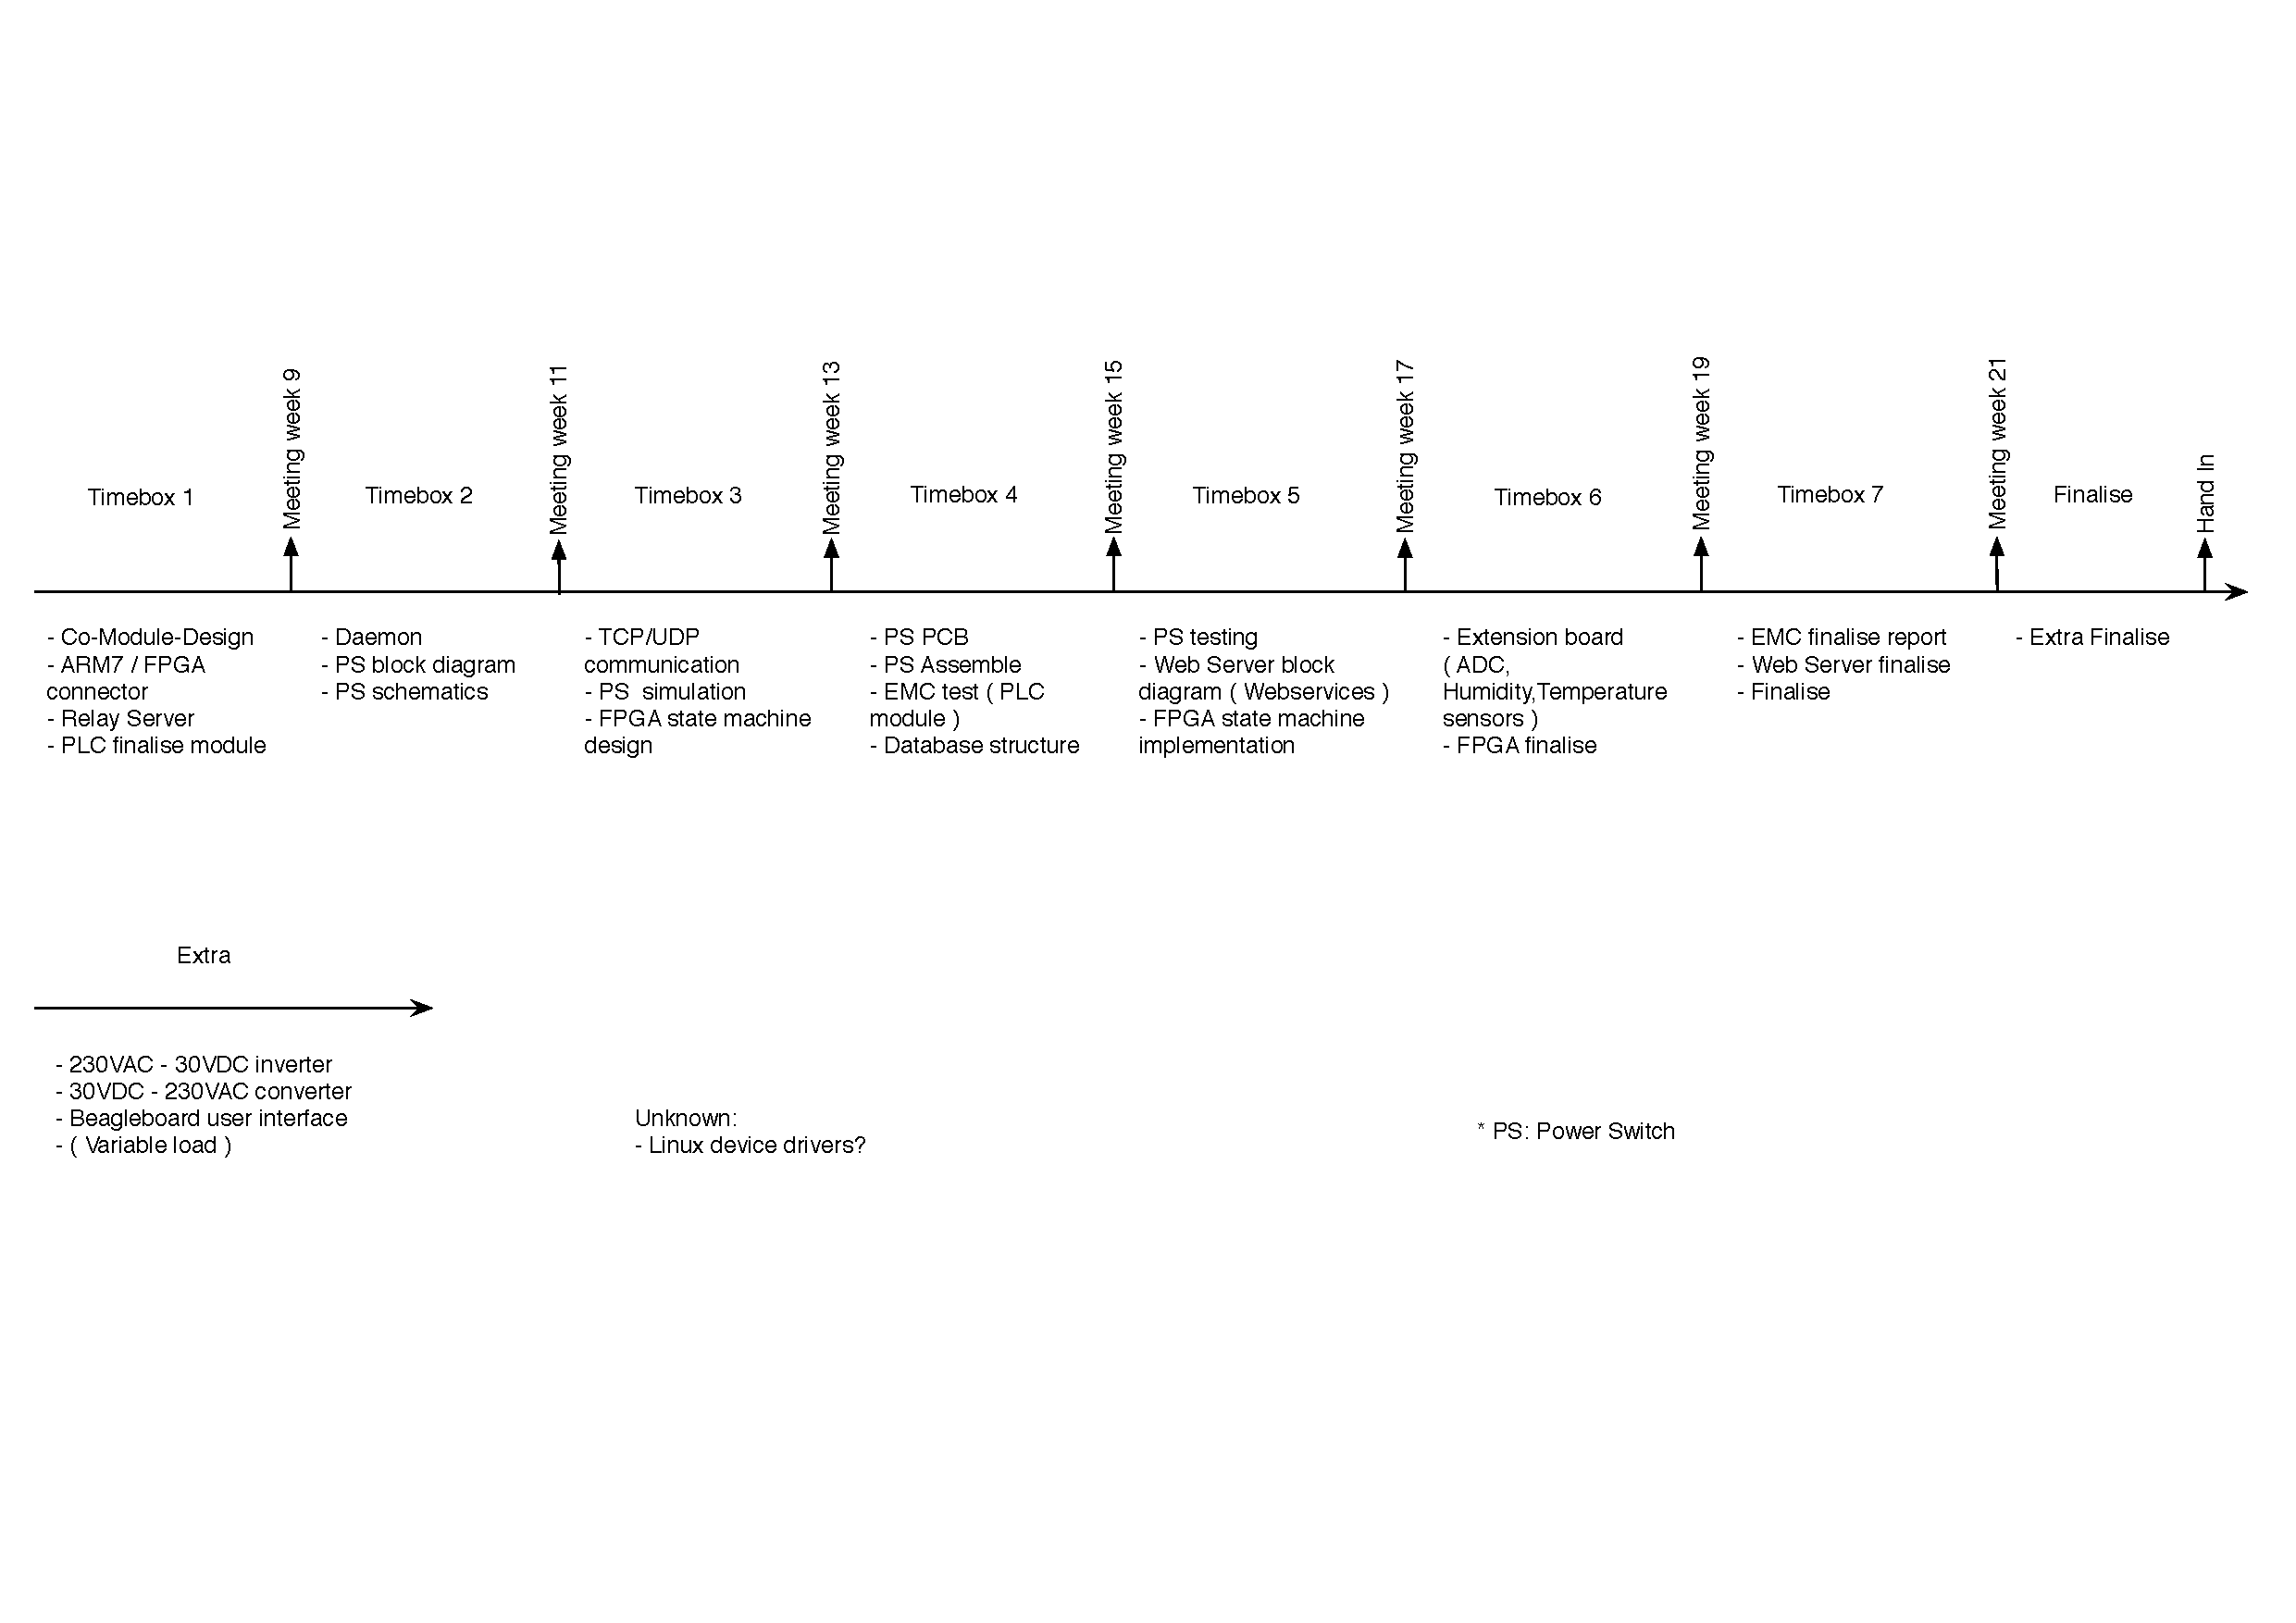
\includegraphics[width=1.0\textwidth]{images/tb_r1.pdf}
		\caption{Outline of the time-boxes}
	\end{centering}
\end{figure}

\subsubsection{Work to be done in this time box}
\begin{itemize}
	\item CO-Module-design
	\item Print connector (connector board between the FPGA board and the ARM board used).
	\item Relay server
	\item PLC module (Power line module for communication between the modules)
\end{itemize}

\subsection{ARM to FPGA connector - Dennis}
Connecting the FPGA board (in our case a Spartan6 board by Digilent and the Arm board from EA) can be done in different ways. The fastest way if the number of connections are relatively low, is usually with a bunch of wires between the two boards. But even though such a setup can be much more flexible, it can be very hard to error searching if something is not working (because of a broken wire or a short circuit) and is also very sensitive to noise. Instead of the wires a PCB solution has been chosen, which will be designed to fit between the two bords pin headers. By placing the boards next to each other an approximation of the board size is found. Size of the board is set to 16 x 5 cm. The connections available on the FPGA boards extension pins is 28, so a 32 bit connection is not a possibility, instead a 16 bit data connection is chosen. The pins routed between the ARM and the FPGA is:
\begin{itemize}
	\item 16 x Data
	\item 7 x Address
	\item 1 x Chip select
	\item 1 x Write enable 
	\item 1 x Output enable (read enable)
	\item 1 x interrupt to the ARM processor
	\item 1 x Reset from the ARM board
\end{itemize}
The reset pin is used for synchronous reset of the two boards. The interrupt signal makes it possible for the FPGA to interrupt the ARM board. The chip select is used, as two other devices is also connected to the external memory.
\begin{figure}[H]
	\begin{centering}
		 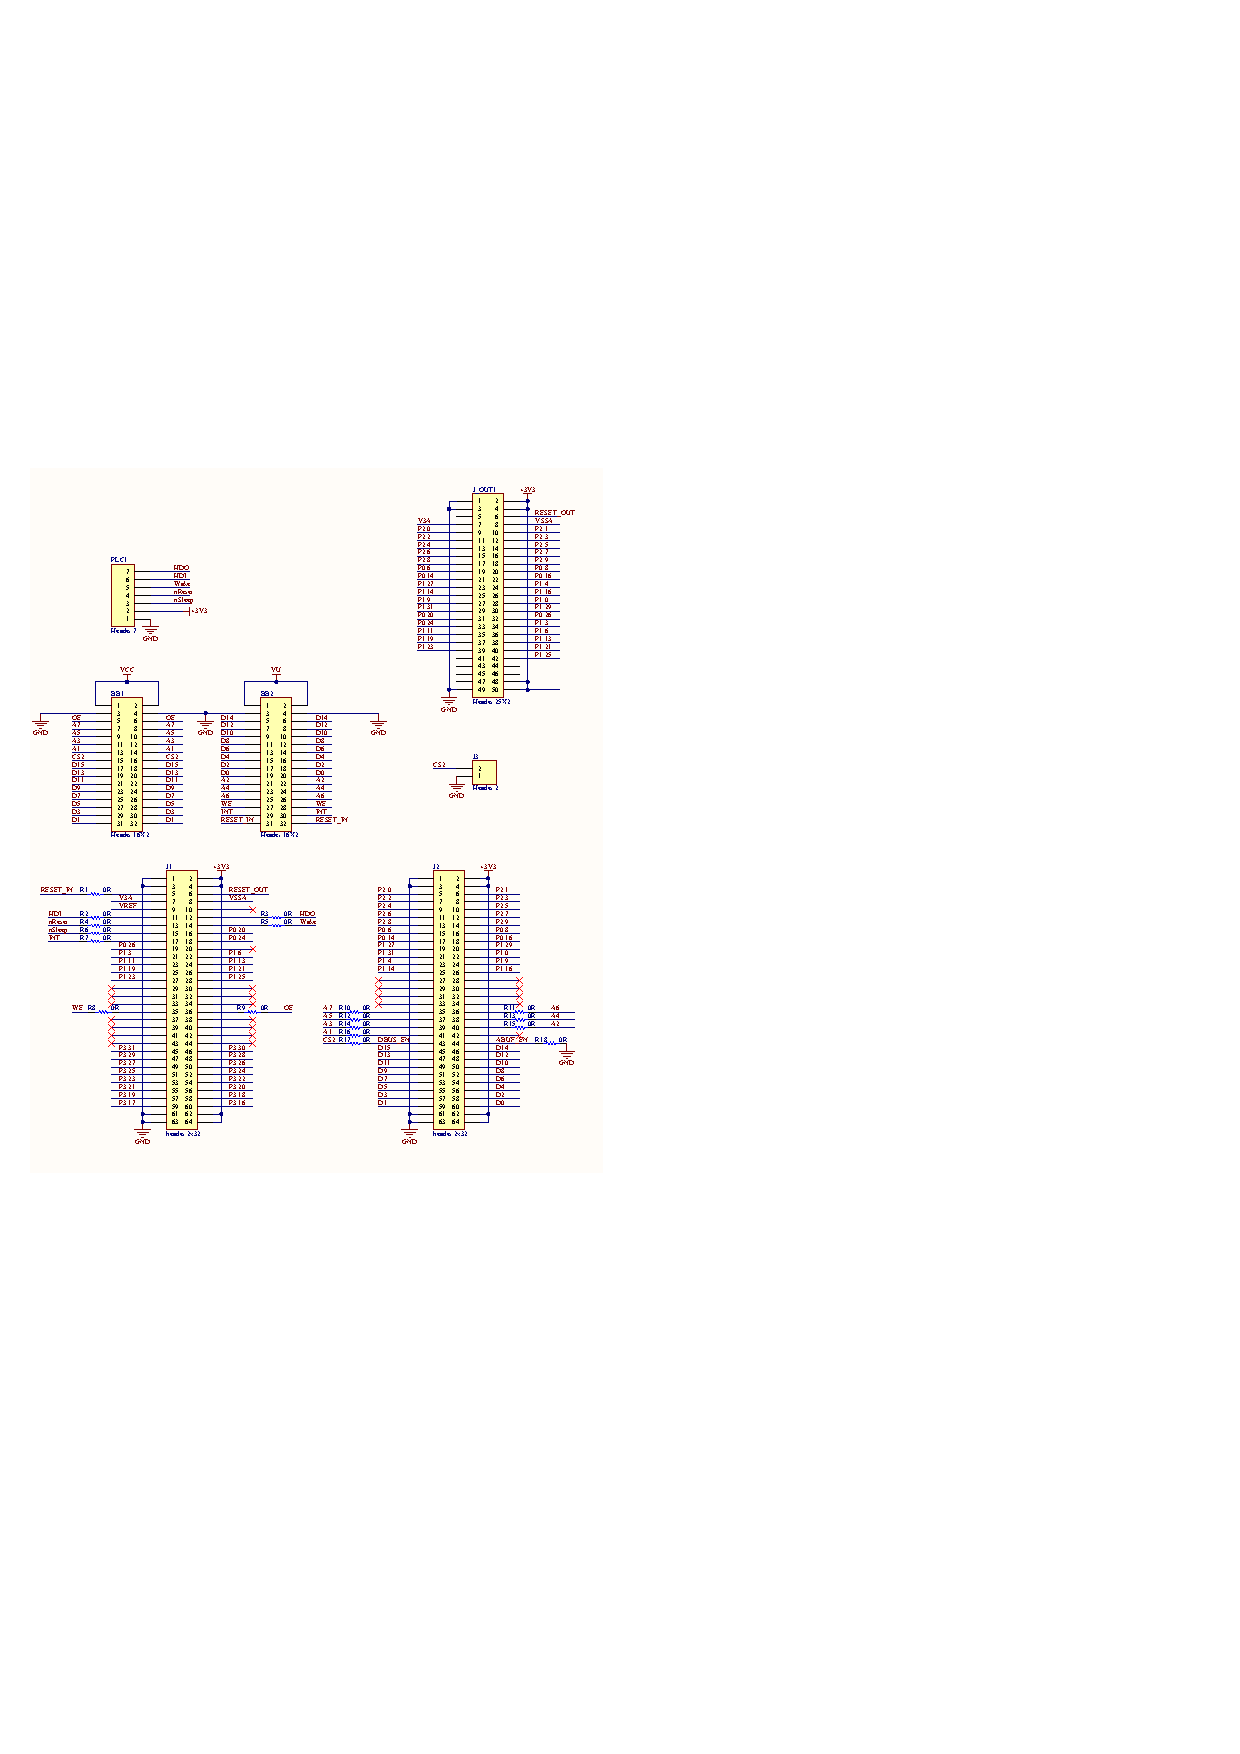
\includegraphics[width=0.60\textwidth,page=1]{images/dig_to_ea_v0_1}
		\caption{Schematic of the ARM to FPGA connector.}
	\end{centering}
\end{figure}
A connector for the power line module is also mounted, to easily interface the module with the ARM processor. An pin header with all the unused pins is also added, to make it possible to quickly connect external devices to the processor. 
\begin{figure}[H]
	\begin{centering}
		 \includegraphics[height=0.8\textwidth,page=2,angle=90]{images/dig_to_ea_v0_1}
		\caption{PCB of the ARM to FPGA connector (top view)}
	\end{centering}
\end{figure}

\subsection{Concurrent design - Theis}
Concurrent design in the design of embedded system is a method to decided where to place different parts of the system, from the specification and performance requirements. The difference between traditional design and co-design is, in traditional design, two groups of experts design independently hardware and software, to implement when all is finish. In co-design one group is designing the whole system and implement the part where they get the best performance and power use.\\
Concurrent design has four steps that is:
\begin{enumerate}
	\item Modelling
	\item Partitioning
	\item Concurrent synthesis
	\item Concurrent simulation
\end{enumerate}
In this time box, only the two first steps are described according to the project time plan.

\subsubsection{Modelling}
In the modelling phase, the customers needs is taking into consideration, and the platform for the system is choose. In this project the platform is specified from the project requirements, to include an ARM7 CPU with uClinux as processor in the system, and a Spartan 6 or 3 FPGA for hardware parts in the system.

\subsubsection{Partitioning}
In "technical platform" from the launch phase, the hardware and software specification was made, and the table below shows which parts of the project that can be implementet both in the ARM7 CPU as software and in the FPGA as hardware.

\begin{itemize}
	\item PLC module
	\item Power switch
	\item A/D Converter
	\item Ethernet
	\item Web server
	\item Interface
	\item Indicator
\end{itemize}
\textbf{PLC module} is used to communicate with the other modules, this part is best implemented in the ARM7 CPU as software, because it is a data-communication protocols.\\
\textbf{Power switch} is used to control the switch and is a rather complex algorithm, it have to be dynamic when controlling the switch, because the power consumption and production is never the same, this part is best implemented in software for the ARM7 CPU.\\
\textbf{A/D Converter} is a very suitable part to implement in the FPGA as hardware, the frequency is high, the memory requirement is small, the task is static. And in this project there is more than one, so it is good to run this part in parallel.\\
\textbf{Ethernet} is made in software, and supported by the linux kernel. The embedded arm board also have a dedicated chip to handle this part.\\
\textbf{Interface/Indicator} is the buttons and LEDs where the user can interact with the system, this is put into hardware, because it is IOs that is best handle in the FPGA for parallel reading the inputs and setting outputs.

\subsection{Relay-server - Paulo}
Relay server is programmed in C++, this application will run on the development platform so remote access to the EA-LPC2478 board becomes possible.

\begin{itemize}
	\item Requirements
	\item Setting the scene
	\item Server data flow
	\item Further Implementation
	\item Documentation (Generated with Doxygen)
\end{itemize}

\subsubsection{Requirements}
The requirements given to the Relay Server are:

\begin{itemize}
	\item FR 1: Able to accept multiple telnet connections
	\item FR 1.1 Shall accept both TCP and UDP connections
 	\item FR 1.2 Shall be able to connect to the daemon on the target
 	\item FR 13 Shall relay traffic unmodified between the telnet client and the daemon
 	\item NF 1: Shall be programmed in C++
 	\item BR 1: Handling more than one connection
 	\item BR 1.1: If more than one active let the others wait - give a message
 	\item BR 1.2 When a blocking connection is terminated the next waiting connection shall be connected to the daemon
\end{itemize}

\subsubsection{Setting the scene}
In this exercise a C program was created as close as possible to what the daemon is supposed to archive.This will give advantages in the daemon programming (Time Box 2) since the communication with the TCP protocol is done.

The "daemon" is a TCP echo server, it sends the same message trough the same socket back to the relay server.

The relay server only forwards messages from the client ( by TCP or UDP ) to the "daemon" without changing any data.

\subsubsection{Server data Flow}

The final server (daemon) is an echo server, it only reply the last received message, this kind of server is used for debug, to be sure the communication is being established. 

\begin{figure}[H]
	\begin{centering}
		 \includegraphics[width=0.8\textwidth,page=2,angle=0]{images/dataflow1.png}
		\caption{TCP Data flow between Client, Server, Daemon - Client connection}
	\end{centering}
\end{figure}

\begin{figure}[H]
	\begin{centering}
		 \includegraphics[width=0.8\textwidth,page=2,angle=0]{images/dataflow2.png}
		\caption{TCP Data flow between Client, Server, Daemon - Client disconnect}
	\end{centering}
\end{figure}

\subsubsection{Further Implementation}

\begin{itemize}
	\item UDP connection not yet implemented in Time Box 1, this will be implemented in Time Box 2.
	\item Implementation of interrupts for read an write on the sockets will improve performance, this will be implemented in Time Box 2 with the "daemon".
\end{itemize}

\subsubsection{Documentation (Generated with Doxygen)}

Documentation can be found in the external document \textit{RelayServer\_Documentation}

\subsection{Power Line module - Dennis}
The documentation of the Power Line module can be found in a separate report called: \textit{EPRO 3 \& 4 PLC - Hardware Interface} as the work is done in corporation with another team. So far the first prototype has been mounted and tested, which has lead to some improvements of the design. The second prototype is ready for mounting and testing which will also be described in the design document. 

\begin{figure}[H]
	\begin{centering}
		 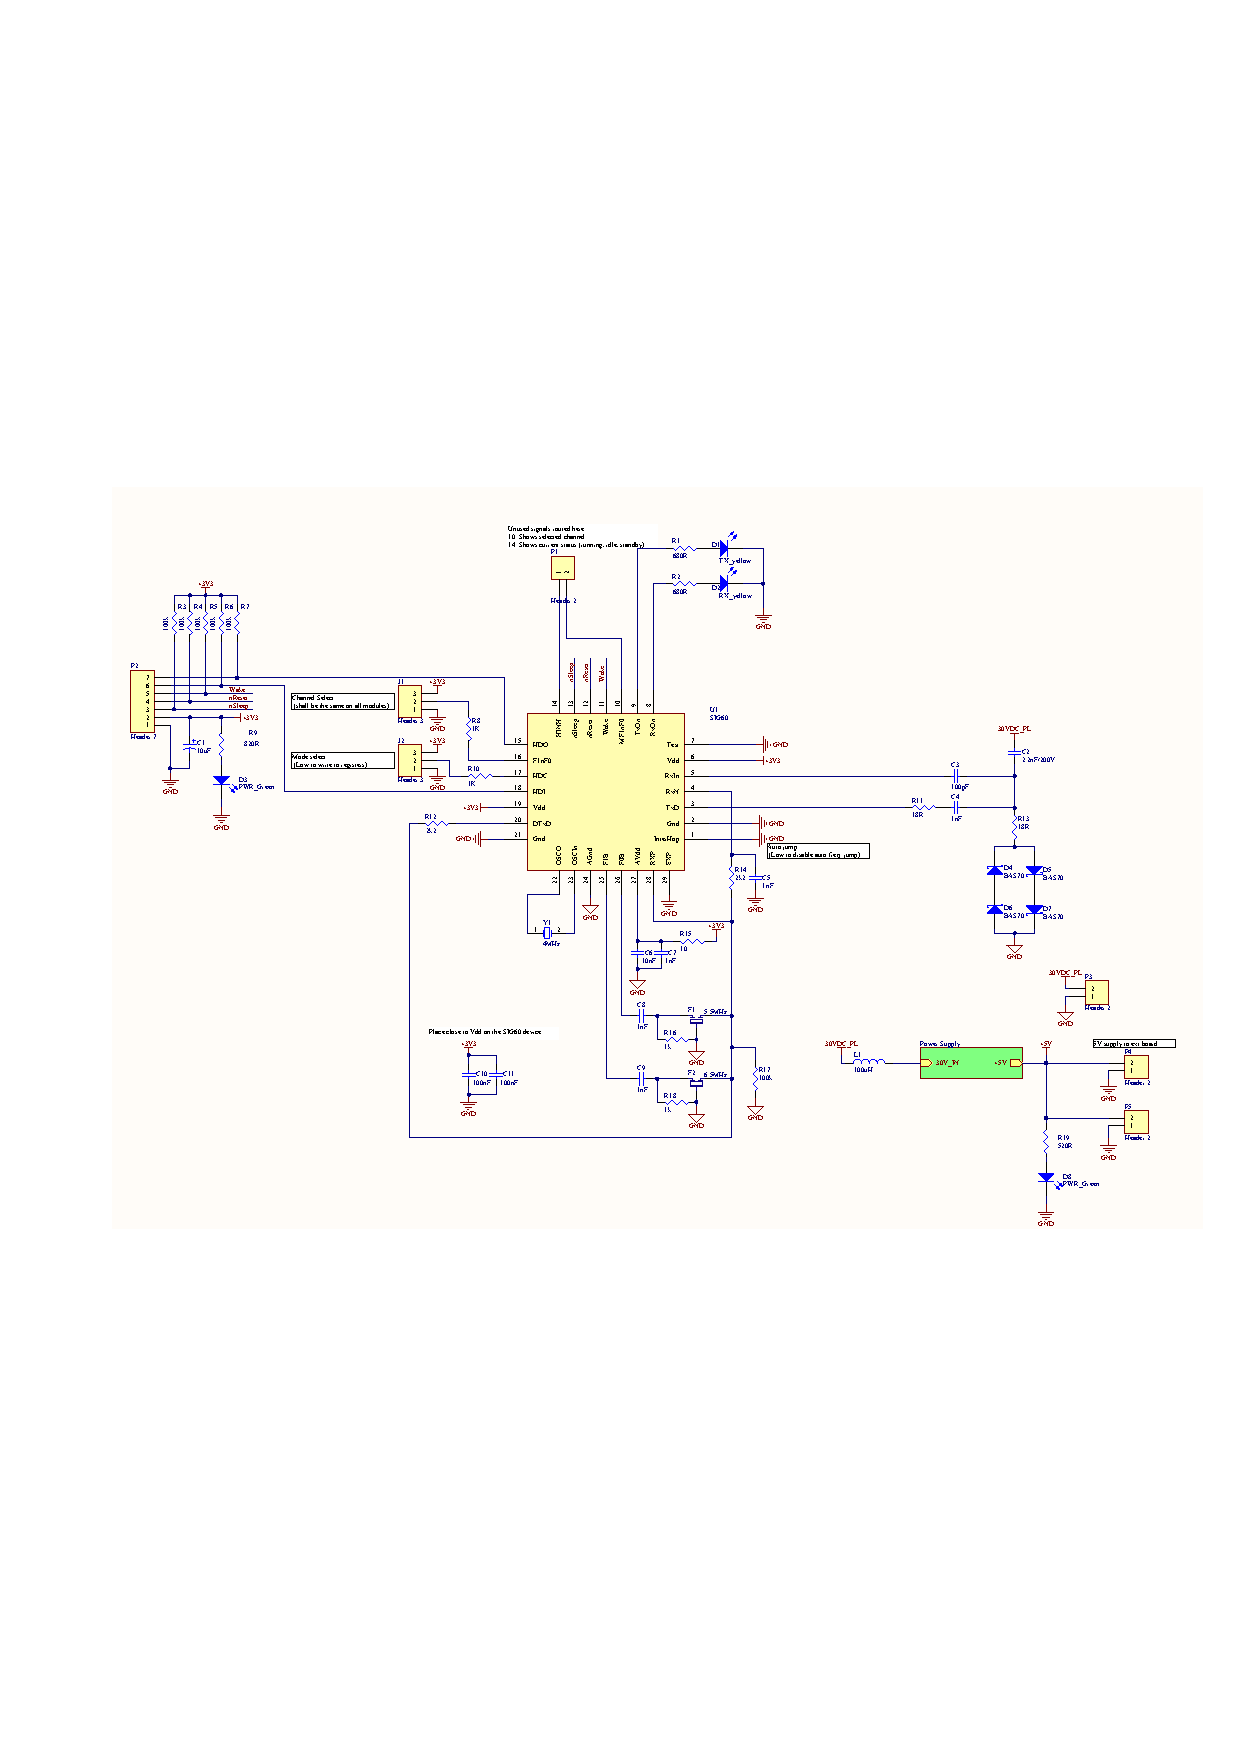
\includegraphics[width=0.9\textwidth,page=1,angle=0]{images/SIG60_v0_2}
		\caption{Power line circuit version 0.2}
	\end{centering}
\end{figure}

\begin{figure}[H]
	\begin{centering}
		 \includegraphics[width=0.8\textwidth,page=2,angle=0]{images/SIG60_v0_2}
		\caption{Power supply. 2 x 5 volt 3 ampere version 0.2.}
	\end{centering}
\end{figure}

\begin{figure}[H]
	\begin{centering}
		 \includegraphics[width=0.8\textwidth,page=3,angle=0]{images/SIG60_v0_2}
		\caption{PCB layout of the power line circuit and the 5 volt power supply version 0.2.}
	\end{centering}
\end{figure}

\newpage
\section{Time box 2}\newpage
%\section{Time box 3}
Show meeting in week 13.
\begin{itemize}
	\item Almost finish complete system
	\item EMC test of PLC module
	\item Power Switch Schematic + Print layout
\end{itemize}\newpage
%\section{Time box 4}
\listoftodos
\subsection{Time box planning}
\begin{figure}[H]
	\begin{centering}
		\missingfigure{Updated timebox figure}
		%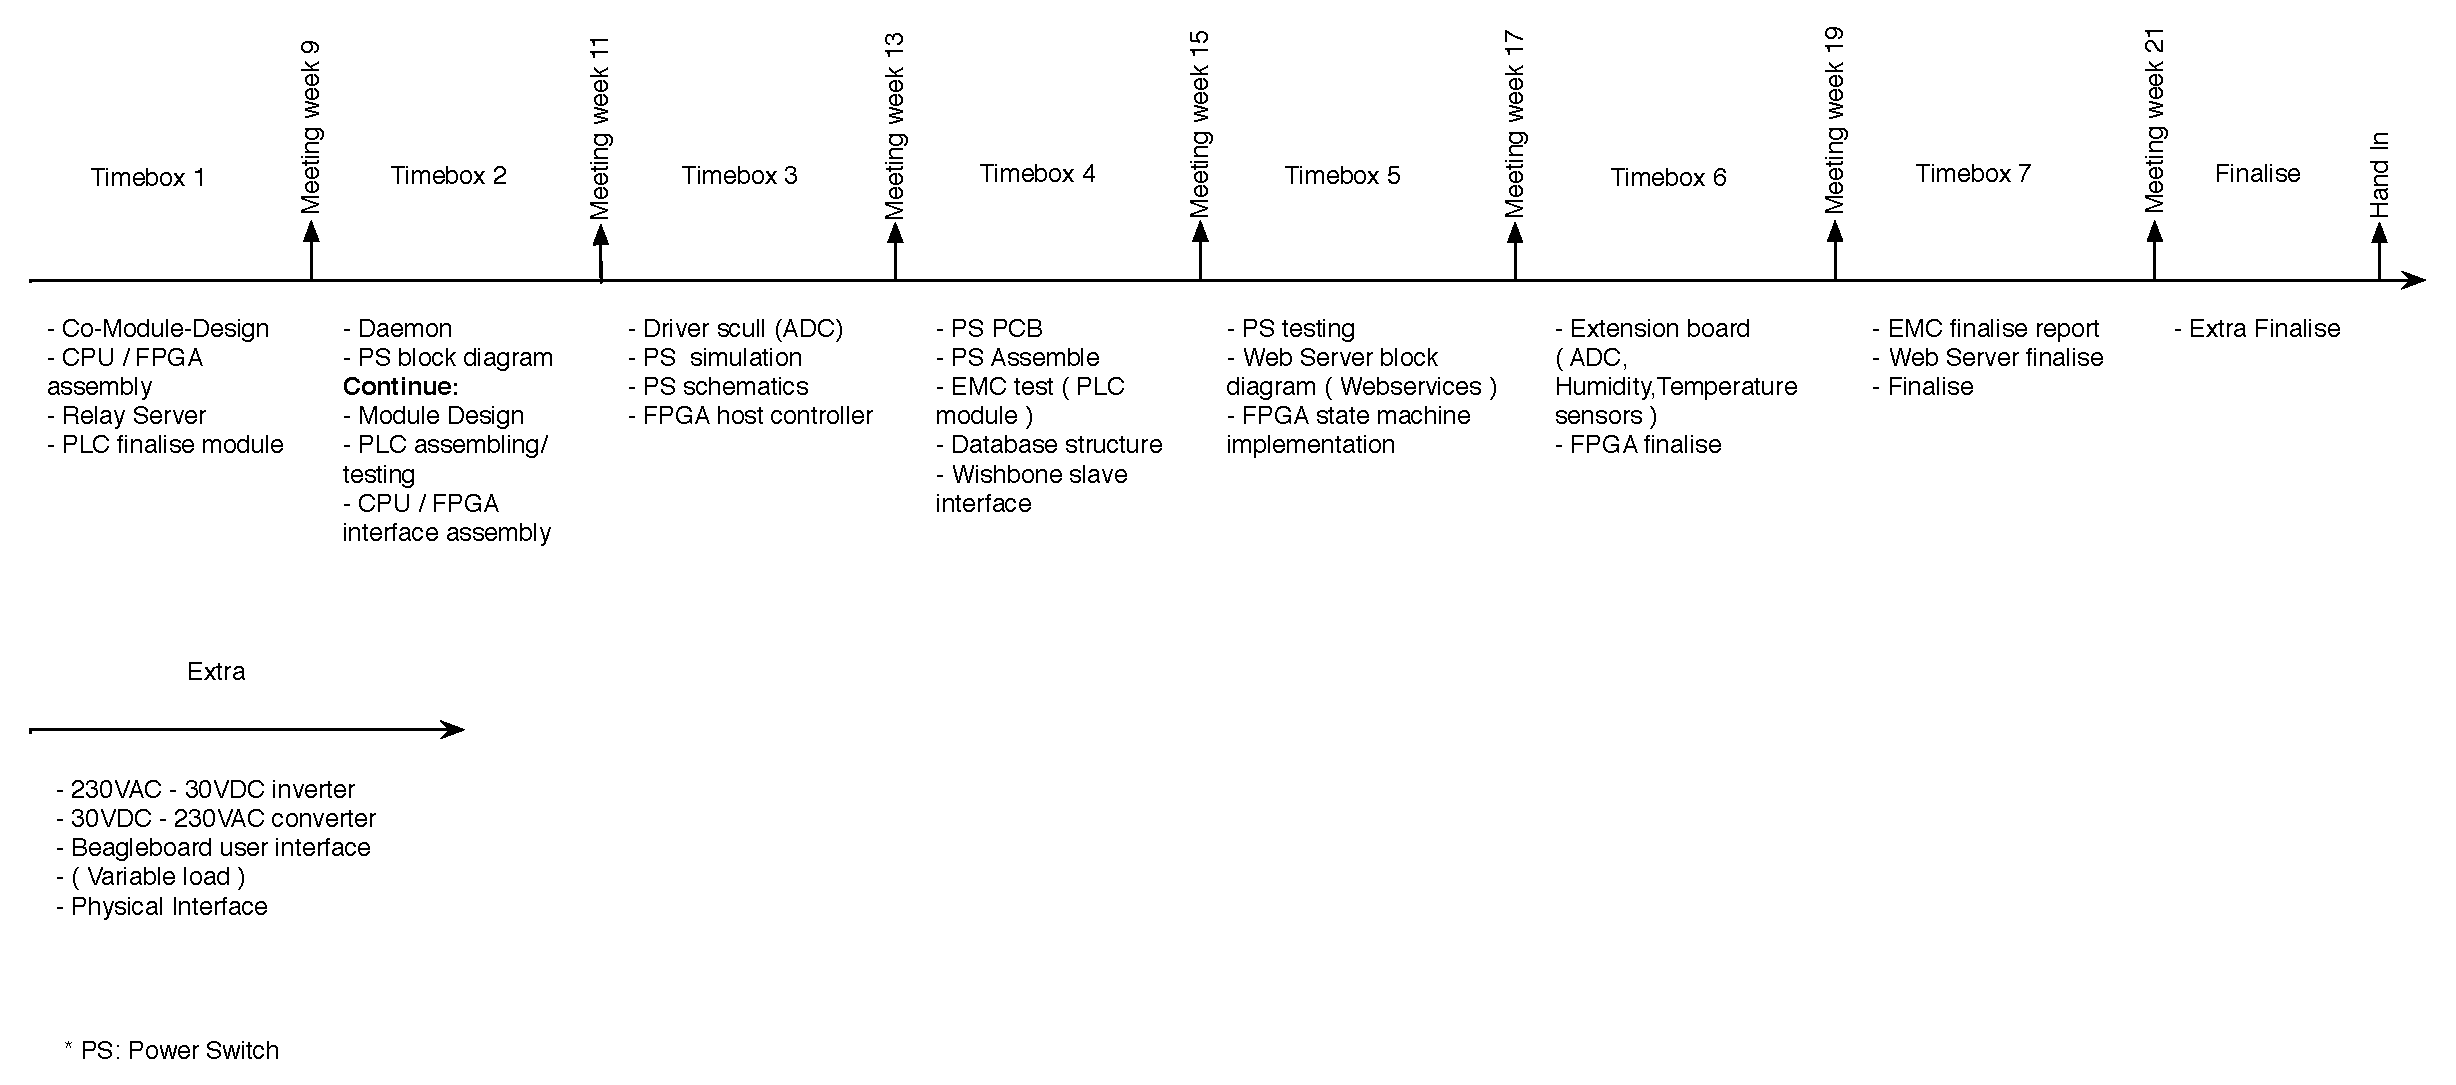
\includegraphics[width=1.0\textwidth]{images/tb_r3.pdf}
		%\caption{Updated time-box}
	\end{centering}
\end{figure}
\subsubsection{Work to be done in this time box}
\begin{itemize}
	\item Power line communication module
	\begin{itemize}
		\item EMC test of modules
	\end{itemize}
	\item Database
	\begin{itemize}
		\item \todo[author=Jesus, inline]{edit what you like and bake a cake}
	\end{itemize}
	\item Physical interface
	\begin{itemize}
		\item Wishbone slave interface
		\item Switch driver
		\item LED driver
	\end{itemize}
\end{itemize}
\paragraph{Description:}
\begin{description}
	\item[Power line module] \todo[author=Dennis, inline]{edit here Dennis}
	\item[Database] \todo[author=Jesus, inline]{edit here Jesus}
	\item[Physical interface] is the light indication and the switches that shall be on the physical hub interface
\end{description}
\subsubsection{Time planning}
\begin{table}[H]
\centering
	\begin{tabular}{|l|c|c|c|c|}
		\hline
		~			& PLC module	& Database	& Physical interface\\ \hline
		Estimation	& xx			& xx		& 12				\\
		Actual		& xx			& xx		& xx				\\
		Developer	& Dennis		& Paulo		& Theis				\\
		\hline
	\end{tabular}
	\caption{Estimation and actual time used on the project}
\end{table}
\subsection{Power line communication module - Dennis}
%			intro
%			
%					verification specification
%					deployment specification
%					
%			Analysis
%	
%	                Refactored block diagram
%	                Refactored class diagram
%	                Detailed use cases
%	                User interface specification
%	                System interface specification
%	                Dimensioning specification 
%	
%	        Design
%	
%	                UML/SysML deployment view(s)
%	                Mechanical specifications and dimensioning
%	                HW module specification per block
%	                UML SW deployment view
%	                Class specification
%	                Refactored class diagram
%	                Use case scenarios specifications
%	                Sequence diagrams 
%	
%	        Implementation
%	
%	                Mechanical drawings with details explained
%	                Electronic diagrams with details explained
%	                Source code with details explained
%	                Description of integration 
%	
%	        Verification
%	
%	                Module tests
%	                Integration tests
%	                Acceptance test
\subsection{Database - Paulo}
%			intro
%			
%					verification specification
%					deployment specification
%					
%			Analysis
%	
%	                Refactored block diagram
%	                Refactored class diagram
%	                Detailed use cases
%	                User interface specification
%	                System interface specification
%	                Dimensioning specification 
%	
%	        Design
%	
%	                UML/SysML deployment view(s)
%	                Mechanical specifications and dimensioning
%	                HW module specification per block
%	                UML SW deployment view
%	                Class specification
%	                Refactored class diagram
%	                Use case scenarios specifications
%	                Sequence diagrams 
%	
%	        Implementation
%	
%	                Mechanical drawings with details explained
%	                Electronic diagrams with details explained
%	                Source code with details explained
%	                Description of integration 
%	
%	        Verification
%	
%	                Module tests
%	                Integration tests
%	                Acceptance test
\subsection{Physical interface - Theis}
%			intro
%			
%					verification specification
%					deployment specification
%					
%			Analysis
%	
%	                Refactored block diagram
%	                Refactored class diagram
%	                Detailed use cases
%	                User interface specification
%	                System interface specification
%	                Dimensioning specification 
%	
%	        Design
%	
%	                UML/SysML deployment view(s)
%	                Mechanical specifications and dimensioning
%	                HW module specification per block
%	                UML SW deployment view
%	                Class specification
%	                Refactored class diagram
%	                Use case scenarios specifications
%	                Sequence diagrams 
%	
%	        Implementation
%	
%	                Mechanical drawings with details explained
%	                Electronic diagrams with details explained
%	                Source code with details explained
%	                Description of integration 
%	
%	        Verification
%	
%	                Module tests
%	                Integration tests
%	                Acceptance test\newpage
%\section{Time box 5} 
%\listoftodos
\subsection{Time box planning}
\begin{figure}[H]
	\begin{centering}
		%\missingfigure{Updated timebox figure}
		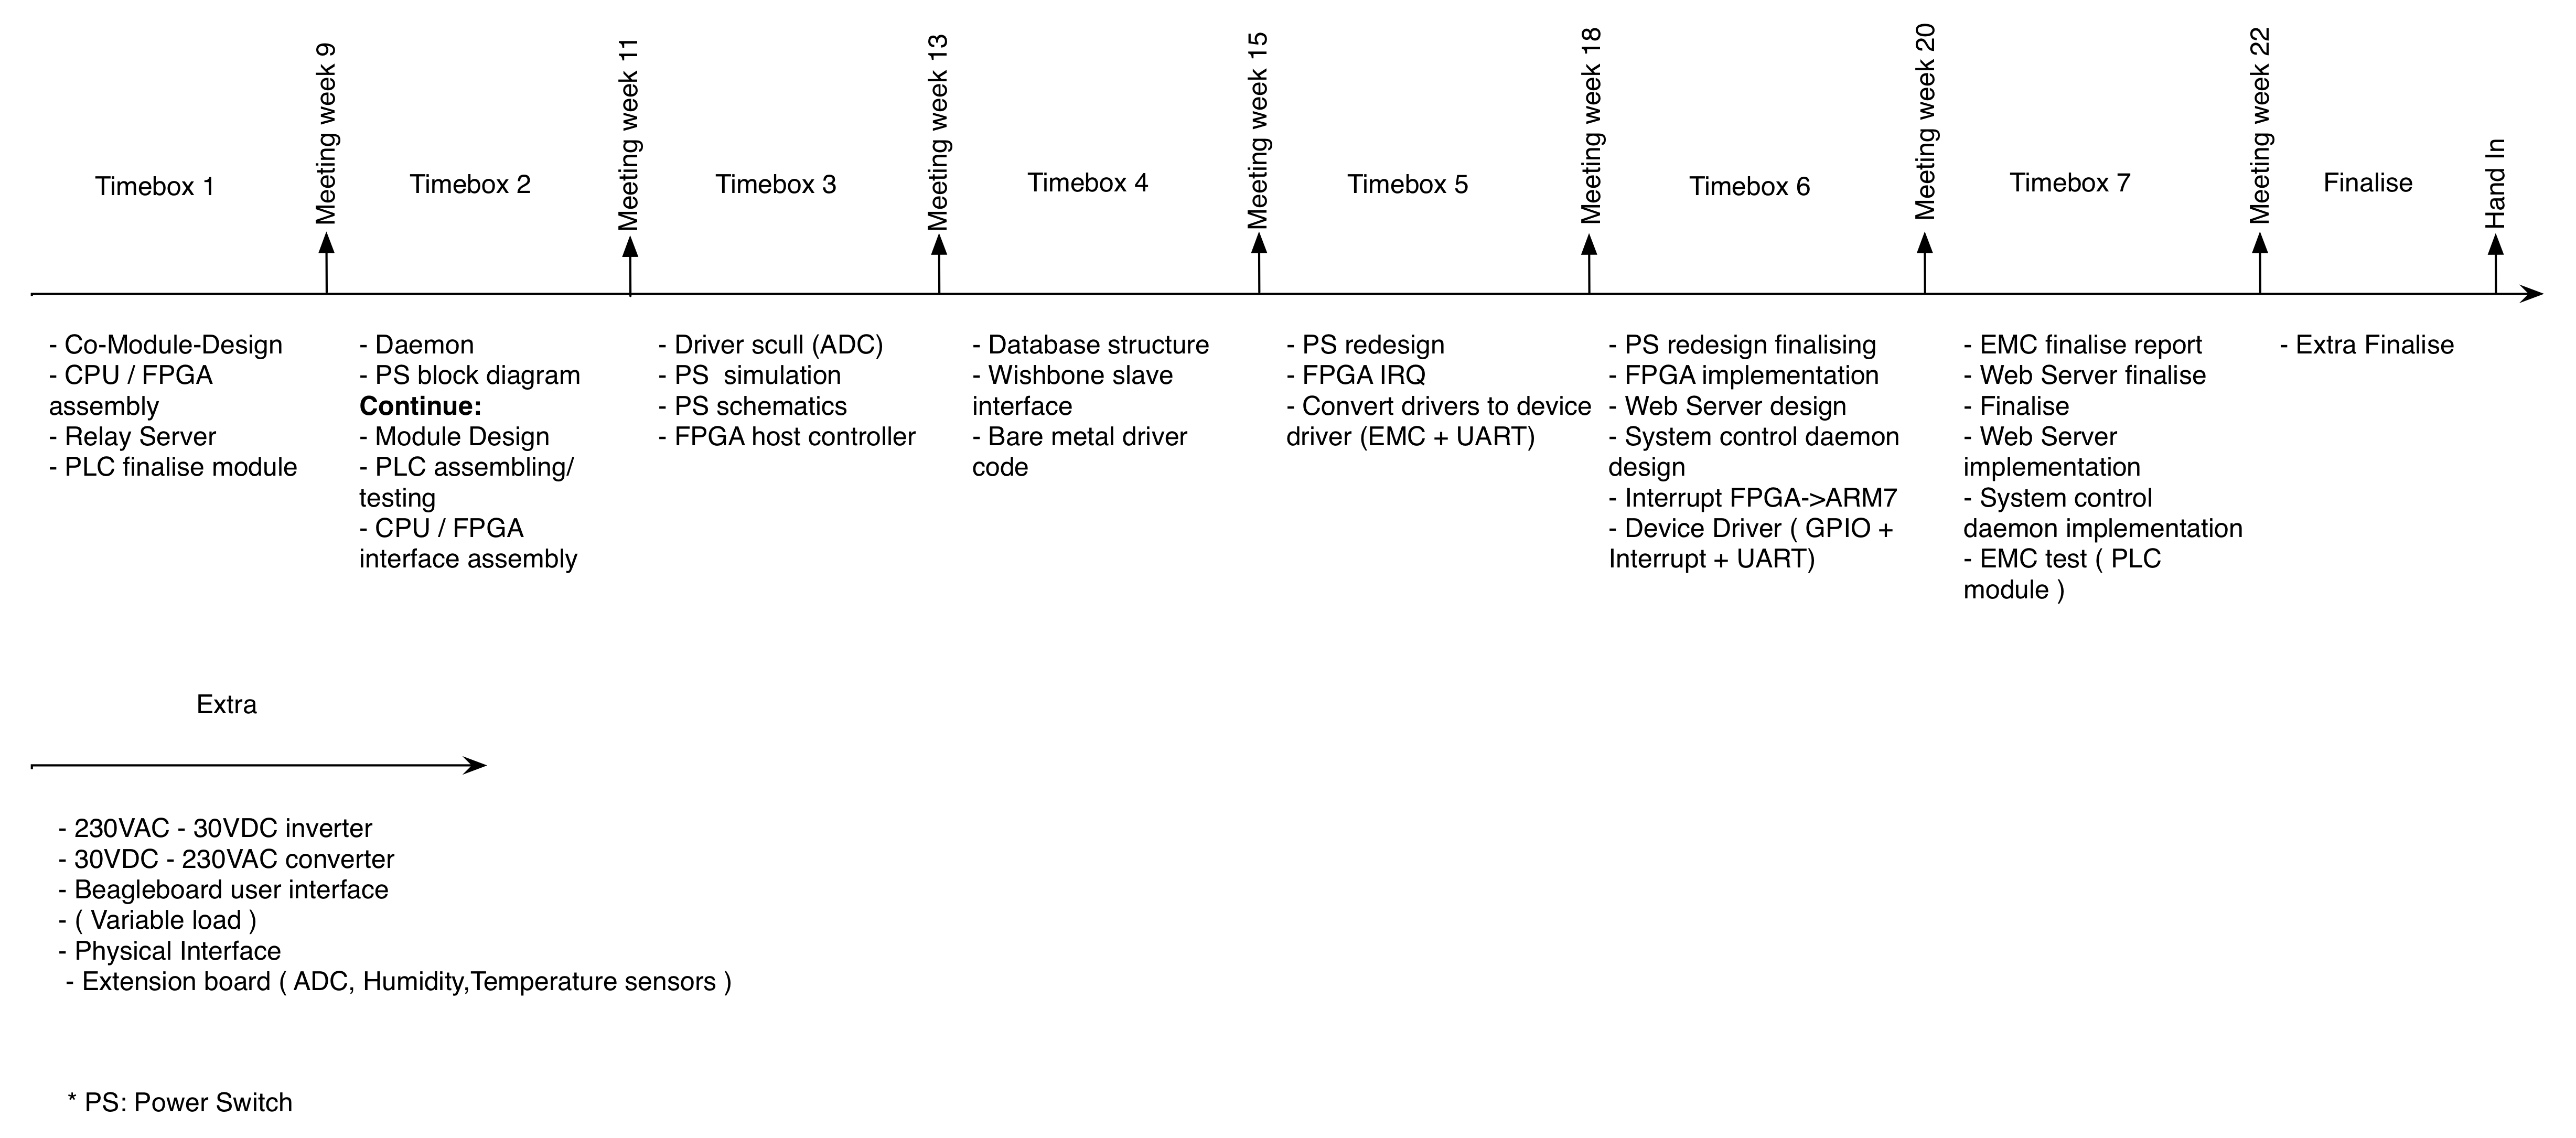
\includegraphics[width=1.0\textwidth]{images/tb_r5.png}
		\caption{Updated time-box}
	\end{centering}
\end{figure}
\subsubsection{Work to be done in this time box}
\begin{itemize}
	\item Power Switch module redesign
	\begin{itemize}
		\item Improvements
		\item Simulation
		\item Redesign
	\end{itemize}
	\item UART Device driver
		\begin{itemize}
			\item Convert UART bare-metal driver into Linux device driver
		\end{itemize}
	\item Interrupt register
	\begin{itemize}
		\item Wishbone slave interface
		\item Interrupt signals
		\item Interrupt handling
	\end{itemize}
\end{itemize}
\paragraph{Description:}
\begin{description}
	\item[UART Device driver] Convert the bare-metal UART driver from the last time box into a device driver, in order to be able to access the UART hardware from user space in the uClinux environment.
	\item[Power Switch] Main component of the energy hub system, controls the ports for each module allowing energy to flow in both directions.
	\item[Interrupt register] is a block in the Spartan 6, that is allow to interrupt the ARM7 directly. The register is handling other interrupts from the Spartan 6 and tell the ARM7 where the interrupt came from.
\end{description}
\subsubsection{Time planning}
\begin{table}[H]
\centering
%	\todo[inline]{Update time}
	\begin{tabular}{|l|c|c|c|c|c|}
		\hline
		~			& UART Device driver	& PS redesign		& Interrupt Register	& Platform setup\\ \hline
		Estimation	& 8						& 17				& 15				& 0			  \\
		Actual		& 22					& 20				& 25				& 11		  \\
		Developer	& Dennis				& Paulo				& Theis				& Dennis	  \\
		\hline
	\end{tabular}
	\caption{Estimation and actual time used on the project}
\end{table}

\subsection{Power Switch redesign}
The prototype made in time box 3 for the power switch module didn't work as expected. New analyses and contact with Linear Technologies revealed that the IC being used (LTC4357) is not the adequate device for this functionality.

\lineparagraph{Requirements}
\begin{itemize}
	\item Voltage input to the Energy hub shall be at 30V $ \pm10\% $
	\item Ampere input to the Energy hub shall be max 30A.
	\item Power-line communication is used, for communication between the different devices and the hub.
\end{itemize}

\lineparagraph{Verification}
\begin{itemize}
	\item The system is able to switch the voltage as input or output. ( Using a Multimeter on both POWERLINE and MODULE connection)
	\item Over voltage and under voltage are keep as set in common requirements 30V $ \pm10\% $ ( Using a Multimeter on both POWERLINE and MODULE connection)
	\item Measurement of the current sensor for calculation of efficiency and security, max 30A. ( Using a Multimeter on the current sensor output pin.)
	\item Create test-bench for 2 PCB switching system. ( Fast prototyping using the mBed )
	\item Test Power Line Communication through the switching system, using development boards from Yamar and mBed.
\end{itemize}
%	Intro
%
%		verification specification
%		deployment specification
%
\subsubsection{Analysis}
%
%	Analysis
%
%                Refactored block diagram
%                Refactored class diagram
%                Detailed use cases
%                User interface specification
%                System interface specification
%                Dimensioning specification 
%
\lineparagraph{Power switch control}
One of the problems found on the first prototype was that the LTC4357 device don't have a control pin to turn the MOSFETs on/off, this device will work only as an ideal diode, making it a good application for photovoltaic harvesting method.

In contact with Linear Technologies a new device was suggested, the LTC4365, this device is a N-Channel MOSFET controller that protects the load using a higher and lower threshold voltage, along with a shut-down pin that drives the MOSFETs gate high or low.

\begin{figure}[H]
	\begin{centering}
		%\missingfigure{Updated timebox figure}
		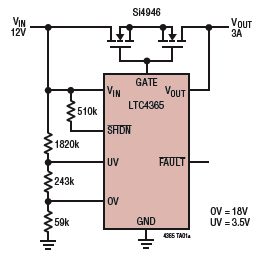
\includegraphics[width=0.5\textwidth]{images/ltc4365.png}
		\caption{LTC4365 application notes.}
	\end{centering}
\end{figure}
In this application the shut-down pin is always high, energy will flow through the MOSFETs when the input voltage is between the under-voltage and over -voltage threshold selected values, in this case 3.5V and 18V.
%
It's necessary to define the over and under-voltage threshold values for the power switch system, this is specified in the common requirements.\\
\\
Common requirements:\\\\
$V_{in} = 30V$ \\
$Offset = \pm 10\% $\\
\\
From the datasheet:\\\\
$ I_{UV} = 10nA $ \\
$ V_{OS} = 3mV $\\
\\
$V_{OSUV}$: maximum tolerable offset (error)\\
$I_{UV}$: worst case scenario current leakage.\\
\\
Under voltage requirement:\\\\
$ U_V=30V-(30*10\%)=27V $\\
\\
Over voltage requirement:\\\\
$ O_V=30V+(30*10\%)=33V $\\
\\
For working conditions of the device the bellow equation have to be true:\\\\
$ R_3+R_4=\frac{V_{OSUV}}{I_{UV}} $\\
\\
Using the formulas given in the datasheet to calculate the value of the 2 resistive dividers:\\\\
$ R_2 = 2*\frac{3mV}{10nA}*(27V-0.5V) = 15.9M\Omega $ Approximate 16M $\Omega $\\ 
\\
$ R_4 = \frac{\frac{V_{OSIU}}{I{UV}}+R_3}{2*O_V} = 246.97k\Omega $ Approximate 250k $\Omega $\\ 
\\
$ R_3 = \frac{V_{OSUV}}{I_{UV}}-R_1 = 50k\Omega $\\
\\
%
\lineparagraph{Simulations}
Linear Technologies have a simulator for their devices, the LTSpiceIV, it's a free software that can be downloaded from the web site.
Using LTSpice to draw a schematics, a test can be performed for the LTC4365 with the required resistor values to the power switch system.
%
\begin{figure}[H]
	\begin{centering}
		%\missingfigure{Updated timebox figure}
		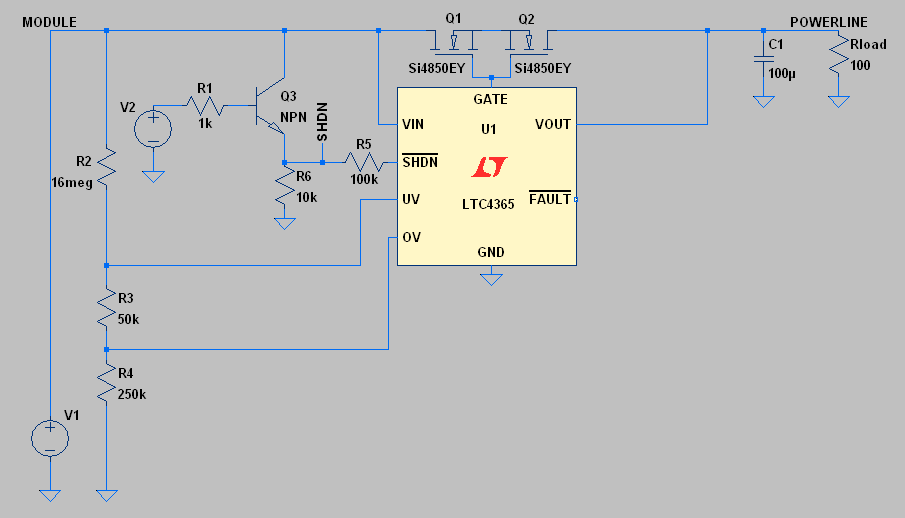
\includegraphics[width=1\textwidth]{images/tb5_LTC_simu1.png}
		\caption{Schematics for the device LTC4365}
	\end{centering}
\end{figure}
%
A NPN transistor is add to drive the shut-down pin high and low. Two N-channel MOSFETs are connected back to back to stop the voltage from passing to the load when the device is shut down.
%
\lineparagraph{Case Scenario 1 ( Producer device connected to the MODULE side )}
\begin{figure}[H]
	\begin{centering}
		%\missingfigure{Updated timebox figure}
		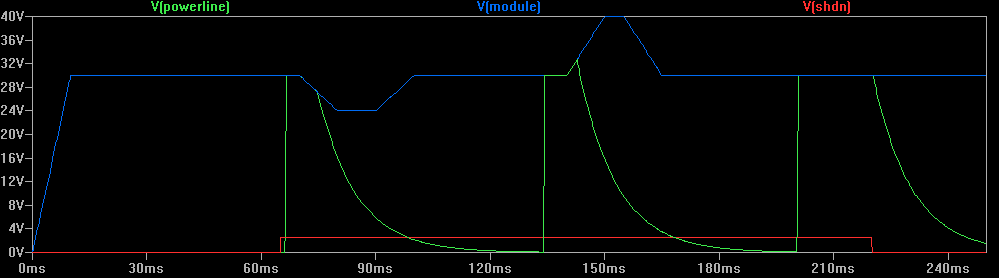
\includegraphics[width=1\textwidth]{images/tb5_LTC_case1.png}
		\caption{Simulation case scenario 1}
	\end{centering}
\end{figure}
In this case scenario the under voltage and over voltage can be tested along with the shut down pin.\\
The simulation has a total time of 250ms, the system takes 10ms to stabilized at 30V which will stabilize the device at that voltage.\\ 
At 65ms the NPN transistor is high, driven the input voltage to the shut down pin, with the shut down pin high the device will drive the gates for the two MOSFETs high and the current will flow through the MOSFETs from MODULE to POWERLINE as expected.\\
The voltage at the module at 80ms is changed to 24V, this will test the under voltage threshold value. From the calculations made in the analysis section, the device should sink the gates to ground when the voltage is under 27V, this happens with success at 75ms as it can be seen in the simulation.\\
To simulate test the over-voltage protection, the MODULE (source) is set to 30V so the device can stabilize again. At 140ms the voltage is pull up to 40V, which the device should sink the gates of the MOSFETs when the voltage is 33V, this happens with success at 142ms.\\
To test the control of the shut down pin, the voltage on the source side is set to 30V, getting the device to stabilize again. With the device in working conditions the NPN transistor is turned off at 220ms, the shut-down pin is then pull down by a 10k$ \Omega $ resistor, pulling the MOSFETs gates to ground\\ 
%
\lineparagraph{Case Scenario 2 ( Device off, no energy flow from MODULE to POWELINE and the other way around )}
In the case scenario 1, there is no energy flowing when the device is off, is necessary now to simulate if the device is working as a diode, if no energy flows in the opposite direction. In this simulation the source and load positions are changed.
\begin{figure}[H]
	\begin{centering}
		%\missingfigure{Case 2 Schematics changed}
		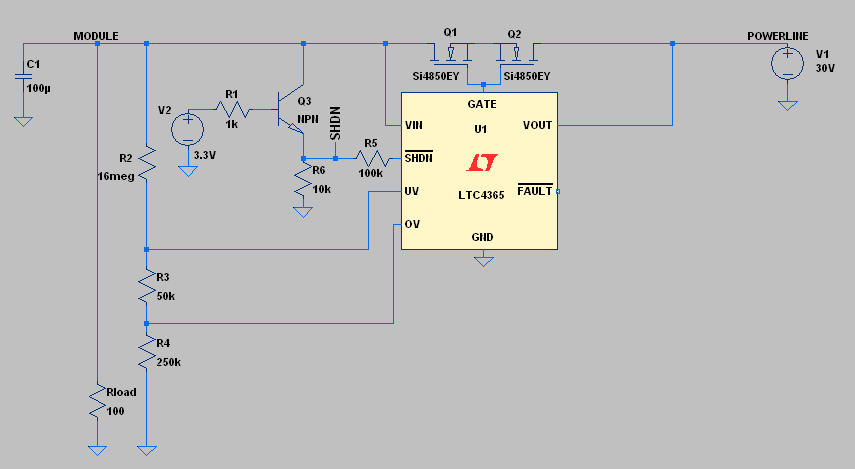
\includegraphics[width=1\textwidth]{images/tb5_LTC_simu2sc.png}
		\caption{Schematics for the device LTC4365 with Case scenario 2 specifications}
	\end{centering}
\end{figure}
%
Being now the POWERLINE the source and the MODULE the load, this situation can occurs when a battery is fully charged and there is a different potential higher on the POWERLINE side. The device is going to insure that no energy flows in the opposite direction. This is successfully shown in the simulation bellow.
%
\begin{figure}[H]
	\begin{centering}
		%\missingfigure{Case 2 Simulation}
		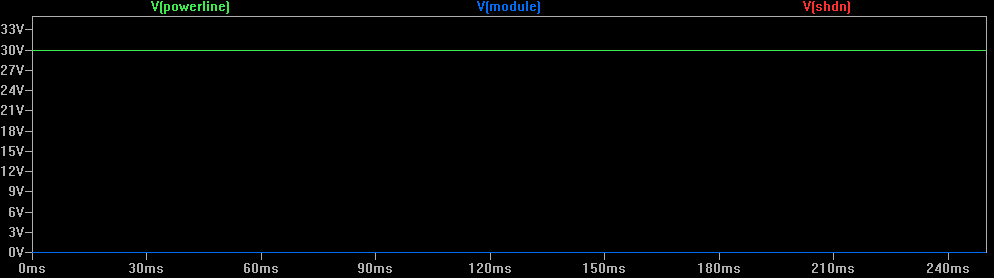
\includegraphics[width=1\textwidth]{images/tb5_LTC_simu2.png}
		\caption{Simulation for case scenario 2}
	\end{centering}
\end{figure}
%
The voltage at the source (POWERLINE) is kept at 30V, and at the load (MODULE) the voltage is around 0V (1mV), in this configuration the circuit is behaving as expected, when the device is off, and the energy flow in the opposite direction the system behave as a diode, blocking the energy from flowing.
%
\lineparagraph{Current Sensors}	
%
Being part of a green energy system, a current sensor is implemented in this power switch system. The measurement of current allows the system to calculate the efficiency of each module connected to the switch port. The current measurements are shown to the user on the web interface.
\\%
The sensor used is a hall effect linear current sensor from Allegro, the ACS756SCA-050B, a bidirectional hall effect sensor with range from -50A to +50A.
%
\begin{figure}[H]
	\begin{centering}
		%\missingfigure{Updated timebox figure}
		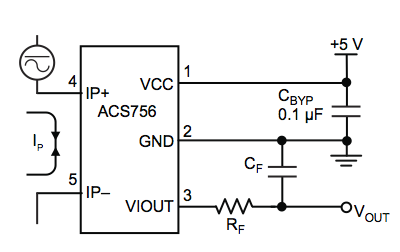
\includegraphics[width=0.5\textwidth]{images/current_sensor.png}
		\caption{ACS756SCA Typical application}
	\end{centering}
\end{figure}
%
A test for this device is set on a bread board, the measurements are made using a voltmeter on the output pin. At a temperature around $ 24^\circ C $ the output increments approximated 40mV for each ampere, this is consistent with the datasheet. \\
Since we can have a meaningful measure with the factory ranges, there is no need to amplify this signal.
%
\begin{figure}[H]
	\begin{centering}
		%\missingfigure{Current sensor set up.}
		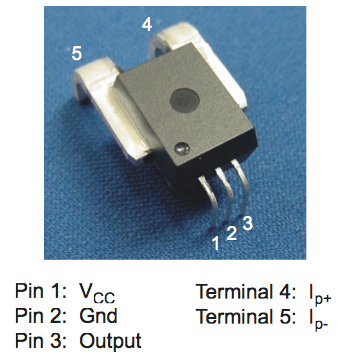
\includegraphics[width=0.40\textwidth]{images/tb5_CS_photo.png}
		\caption{ACS756SCA-050 pins.}
	\end{centering}
\end{figure}
%
\subsubsection{Design}
%
%	Design
%
%                UML/SysML deployment view(s)
%                Mechanical specifications and dimensioning
%                HW module specification per block
%                UML SW deployment view
%                Class specification
%                Refactored class diagram
%                Use case scenarios specifications
%                Sequence diagrams
%
The redesign of the power switch system required some more analysis since this is the main functionality of the energy hub. 
\lineparagraph{Power Switch Overview}
An overview of the system to be can be seen bellow.
%
\begin{figure}[H]
	\begin{centering}
		%\missingfigure{System Block Diagram}
		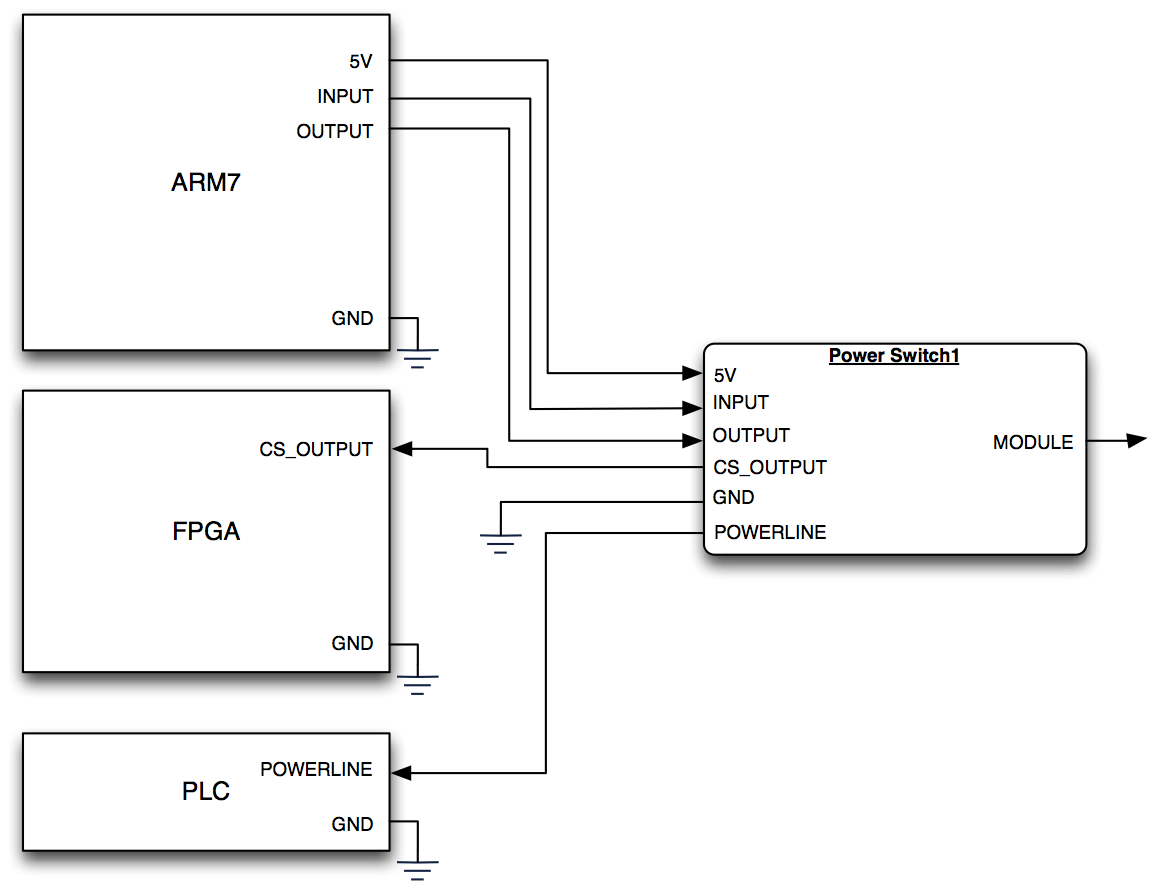
\includegraphics[width=0.90\textwidth]{images/PS_BlockDiagram.png}
		\caption{ACS756SCA-050 pins.}
	\end{centering}
\end{figure}
%
The ARM7 controls the input and output pins of the power switch system, a device driver will be implemented for this functionality later on this project. 
The CS\_OUTPUT corresponds to the current sensor voltage output, with ranges from 0V(-50A) to 5V(50A), this is connected to one of the 8 ADCs implemented on the FPGA and retrieved to the core system (ARM7) through the EMC (External Memory Control) implementation.\\
POWERLINE pin from all power switch systems are connected to the same track into the PLC module. This will work as a sniffer for new communication arriving and to send new communication to the modules connected to the energy hub.\\
The MODULE pin is a connector for each module, in this prototype only 4 ports are built, since there's no more than 4 modules in development.
%
\lineparagraph{Schematics}
Schematics of the power switch system.
\begin{figure}[H]
	\begin{centering}
		%\missingfigure{Current sensor set up.}
		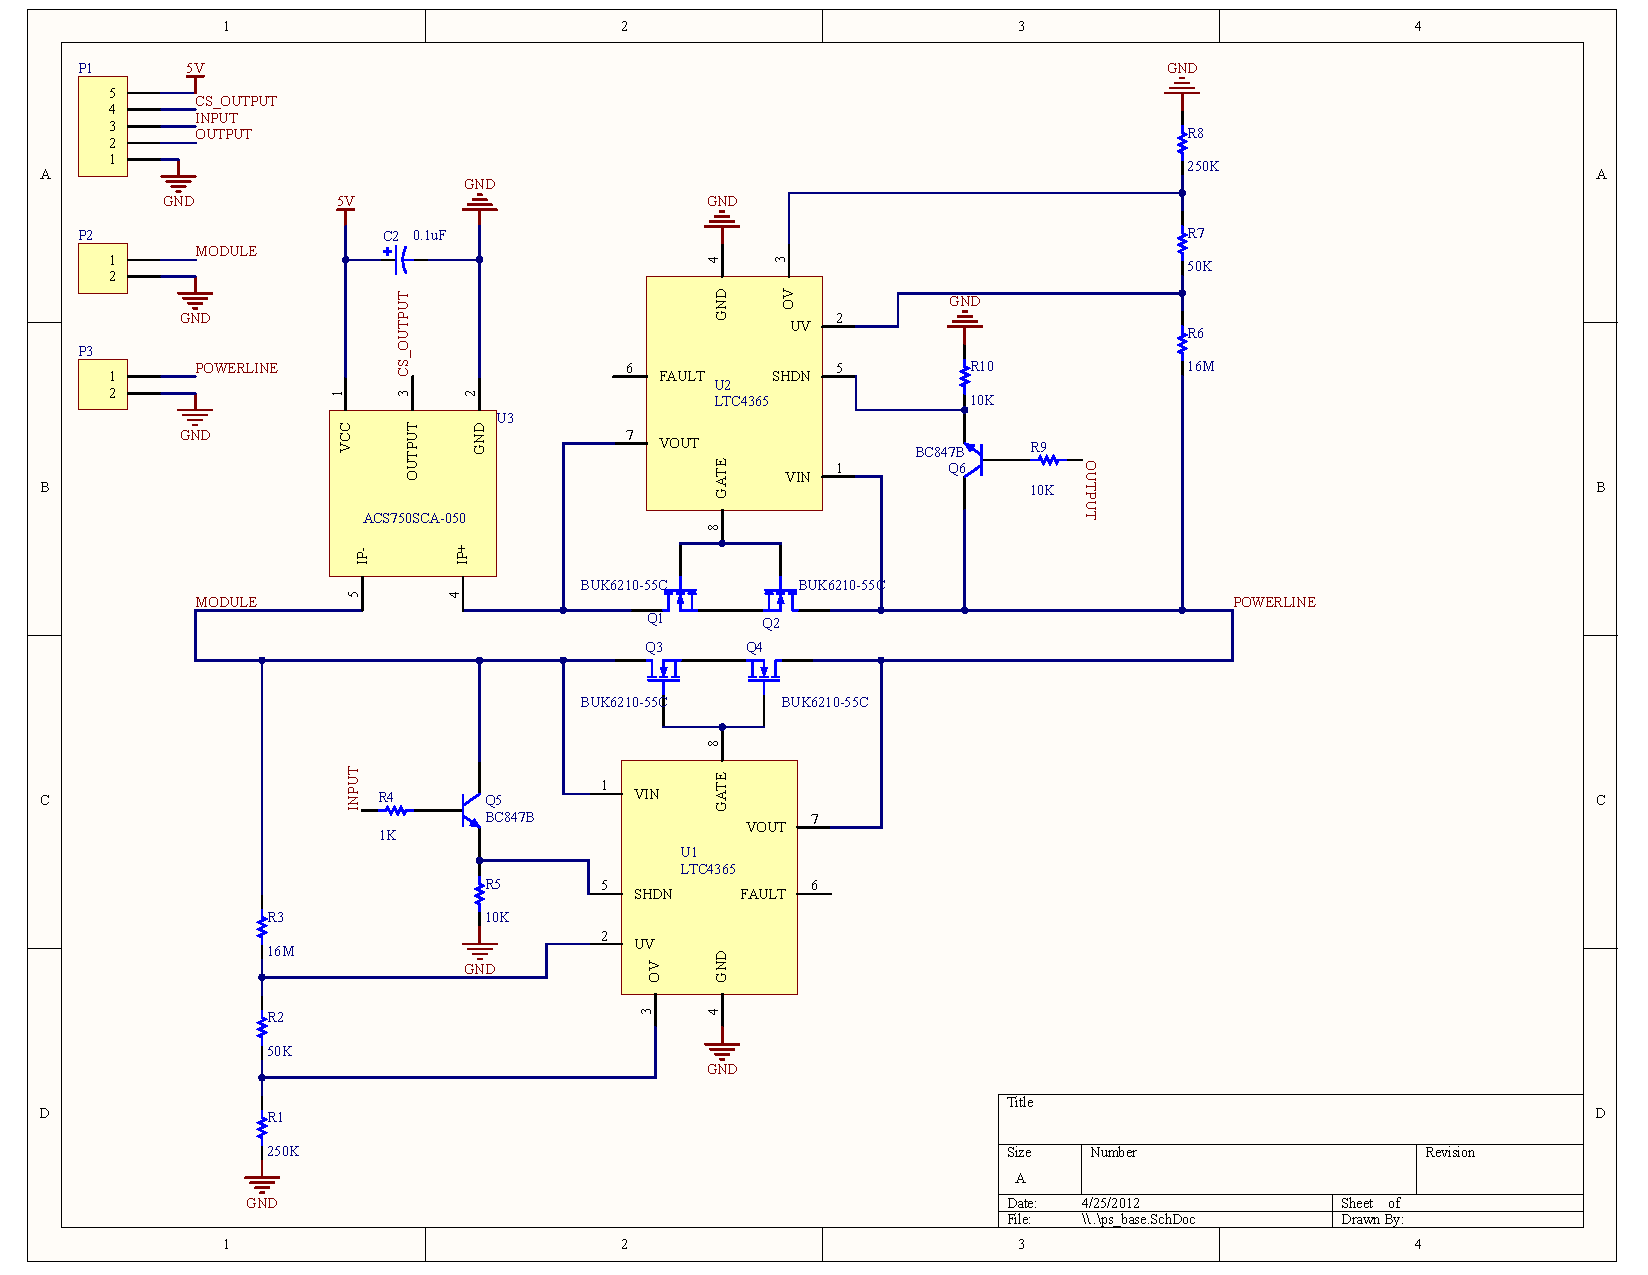
\includegraphics[width=1.0\textwidth]{images/PS_PCB.pdf}
		\caption{Power switch system schematics.}
	\end{centering}
\end{figure}
In this schematics the current sensor is add to the system a long with the new LTC4365 devices to control the two back to back N-channel MOSFETs. A NPN transistor is added between the $ V_{in} $ and the shut down pin, this will drive the pin to the input voltage or connect to ground. \\
In case off power failure the power switch systems are disconnected since the shut down pin is pull down to ground through a 10K$ \Omega $ resistor.
\lineparagraph{PCB layout}
A layout is made using Altium Designer software version 10. 
%
\begin{figure}[H]
	\begin{centering}
		%\missingfigure{PS layout image.}
		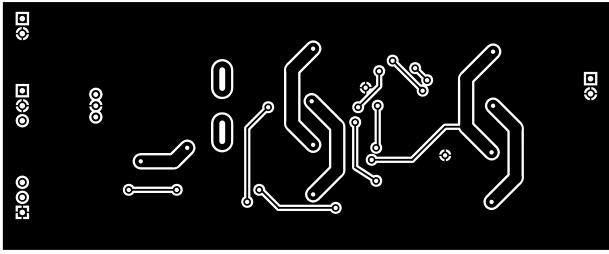
\includegraphics[width=1.0\textwidth]{images/tb5_layout_bottom.png}
		\caption{Power switch layout bottom layer.}
	\end{centering}
\end{figure}
\begin{figure}[H]
	\begin{centering}
		%\missingfigure{PS layout image.}
		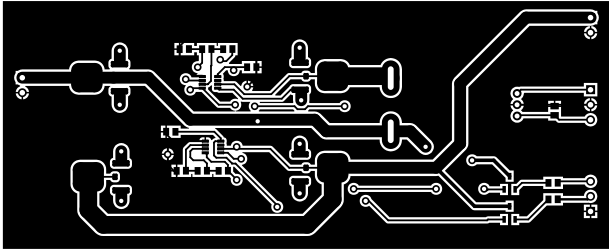
\includegraphics[width=1.0\textwidth]{images/tb5_layout_top.png}
		\caption{Power switch layout top layer.}
	\end{centering}
\end{figure}
%
This layout is a prototype for 1 power switch system, the tracks between the MOSFETs and the pin headers for the modules and power line are larger for eat reduction due to higher current flow.\\
The LTC4365 is as close as possible to the MOSFETs this is suggested in the device datasheet.\\
The board is going to be assembled and tested in time box 6.
%
\subsubsection{Verification}
All the verifications for the power switch system are changed to time box 6 since the PCB will not be ready for testing.
\begin{table}[H]
\centering
	\begin{tabular}{| c | l | c |}
		\hline
		Verification & Description & Acceptance \\\hline
		1 & Switch the voltage as input or output & TimeBox6 \\\hline
		2 & Over voltage and under voltage are kept 30V $ \pm10\% $ & TimeBox6 \\\hline
		3 & Current between maximum 30A & TimeBox6 \\\hline
		4 & Power Line Communication through the switching system & TimeBox6 \\\hline
		5 & 4 PCB switching system & TimeBox6 \\\hline
	\end{tabular}
\end{table}
%
%	Verification
%
%                Module tests
%                Integration tests
%                Acceptance test
%%%%%%%%%%%%%%%%% Dennis Begin%%%%%%%%%%%%%%%%%%%%%%%%%%%%%%%%%%%
\subsection{Platform setup - Dennis} 
A virtual CentOS machine running on a machine at school has been assigned to each team in order to have a host machine where the boot loader (u-boot) can be compiled and modifications to the uClinux kernel can be made. Unfortunately the kernel compiled started to kernel panic. After undoing the different things done (removing files from the rc file and removing different kernel modules) the kernel kept panicking. Instead of using any more time on the machine, another similar virtual machine has been created on a local machine. The virtual machine is running CentOS 5.8 (like the one assigned), fortunately no kernel panic have been detected after compiling the kernel on the "new" local machine. Another benefit by having a local machine up and running is the flexibility as the Embedded Artist board should be connected to the schools network in order to access the tftp server where the board loads the kernel from throughout the development period. Now a tftp server has been set up on the local machine, where to the development board can be directly connected though an ethernet cable.
\subsubsection{Network File system}
In order to speed up the development process of user space applications and device drivers to the board, a NFS server has been setup on the local host machine using the OS X application \textit{NFS Manager}. The NFS disk is then mounted on the board by issuing the command: \\\textit{\#mount -o nolock,rsize=4096,wsize=4096 -t nfs 192.168.1.1:/Users/Shared/nfs\_mount /mnt/nfs}, 
\\which mounts the disk in \textit{/mnt/nfs}. When having the NFS server setup, there is no need to recompile the whole kernel when changes have been done to a kernel module or a user space application before it can be tested on the target. 

\subsection{UART Device driver - Dennis} 
As specified in the Technical platform section, the board used is LPC2478-32 from Embedded Artists. The on-board ARM processor is running uClinux, which is a Linux kernel for micro controllers without a memory management unit. In order to communicate with the UART hardware on the board a device driver has to be written, which is a piece of software that allows user-space applications in the kernel to interface with a hardware device (in this case the UART). The reason why implementing a UART driver, is to be able to communicate with the Power Line module which uses UART interface. 
\begin{table}[H]
\centering
	\begin{tabular}{|p{1.2cm}|p{2.3cm}|p{6cm}|p{6cm}|}
	\hline
	ID		& Requirement		& Description												& Comments\\\hline
	F-1.2		& Communication - System & The hub shall be able to communicate with a connected module through power line communication. & The interface to the power line module is UART.\\\hline
	\end{tabular}
\end{table}
%			Intro
%					verification specification
%					deployment specification
\subsubsection{Analysis}
The UART used for communication to the Power line module is UART2, however instead of making a device driver especially for UART2, a more generic driver is build instead so other UART can be used in the future if there is a need for it. 
\p On the 32 bit LPC2478 processor the UART1 is not supported and UART0 is used as console, so during initialization it is very important not to change in any registers concerning these, to avoid kernel panic or loose communication with the console.
\p The initial framework for the driver was made in the last time box, which will be used as the skeleton together with the bare metal UART driver also made in the last time box. 

%			Analysis
%
%                Refactored block diagram
%                Refactored class diagram
%                Detailed use cases
%                User interface specification
%                System interface specification
%                Dimensioning specification 
\subsubsection{Design}
Before implementing the kernel module, it has to be thought through how to operate with the module from the user side of it. A small test program has been created in order to have some implementation guide lines, but also to have a verification script to all the time test against, to check if the module fulfills all the tests. 
\p The script either opens the /dev/uart2 file and reads it, or opens it and writes the different commands available. After writing the file with one command, the content of the file is deleted (flushed) to prepare for a new operation. 
\begin{lstlisting}[language=c]
#define UART "/dev/uart2"

int main(int argc, char *argv[]) {
        FILE *fp;
	//Write commands
	char buffer1[] = {"INIT:8N1"};
	char buffer2[] = {"BAUD:9600"};
	char buffer3[] = {"WR:55"};
	char buffer4[] = {"WR:0x55"};
	char buffer5[] = {"help"};
	//read buffer
	char read[10];
	//If read is not specified in the arguments do a write
	if(strncmp("read", argv[1], 4) != 0){	//Open the file
		if ((fp = fopen(UART,"wb"))==NULL){
                	printf("Cannot open file.\n");
               	 	exit(0);
        	}
		//Initialize UART2 with 8N1 setup
		fwrite(buffer1, 1, sizeof(buffer1), fp);
		fflush(fp); //Empty the file
		//Define baudrate of devie
		fwrite(buffer2, 1, sizeof(buffer2), fp);
		fflush(fp);
		//Write a value decimal
 		fwrite(buffer3, 1, sizeof(buffer3), fp);
		fflush(fp);
		//Write a value hexadecimal
 		fwrite(buffer4, 1, sizeof(buffer4), fp);
		fflush(fp);
		//Write out different file options
 		fwrite(buffer5, 1, sizeof(buffer5), fp);
        	fclose(fp);
	}
	//Read the file
	else{
		if ((fp = fopen(UART,"rb"))==NULL){
                	printf("Cannot open file.\n");
               	 	exit(0);
        	}
		//Read the file and print it if something available
		if(fread(read,1,10,fp) > 0) printf("\nVAL: %s\n",read);
		else printf("\nFail or nothing to read\n");

		fclose(fp);
	}
        return 0;
}
\end{lstlisting}
As it can be seen in the code, the user has the ability to:
\begin{itemize}
	\item help - get a list of commands available in the kernel module.
	\item WR: - Write a character, which is transmitted on the UART module chosen. The value can be either hex or decimal.
	\item BAUD: - Change the baud rate of a UART to for instance 9600, 115200 or others.
	\item INIT: - Initialize the module with \textit{Word length}, 5,6,7 or 8 bits, \textit{stop bits}, 1 or 2 and \textit{parity bit} on or off. 
\end{itemize}
Note that the first time a device is opened after reset the INIT and BAUD shall be written to it in order to work as wanted. 
%        Design
%
%                UML/SysML deployment view(s)
%                Mechanical specifications and dimensioning
%                HW module specification per block
%                UML SW deployment view
%                Class specification
%                Refactored class diagram
%                Use case scenarios specifications
%                Sequence diagrams
\subsubsection{Implementation}
%%%%%%%%%File Descriptor%%%%%%%%%%%%%%%
As the device has to be able to both read and write, the file descriptor shall at minimum look like below with a open, close, read and write function. Further implementations is discussed in the conclusion section.
\begin{lstlisting}[language=c]
static struct file_operations uart_fops = {
	.owner   = THIS_MODULE,
	.read	 = uart_read,
	.write   = uart_write,
	.open    = uart_open,
	.release = uart_close,
};
module_init(uart_mod_init);
module_exit(uart_mod_exit);
\end{lstlisting}

%%%%%%%%%INIT/EXIT%%%%%%%%%%%%%%%
The init and exit functions are similar to the one used in the ADC, except that the UART2 and UART3 power pins are disabled by default. If these pins are set and reset then the UART devices erases its settings. Therefore the power pins for UART2 and UART3 are set when inserting the module (UART0 and UART1 are enabled at reset).
\begin{lstlisting}[language=c]
m_reg_bfs(PCONP, 0x03000000);
\end{lstlisting}

%%%%%%%%%OPEN/CLOSE%%%%%%%%%%%%%%%
The open and close functions are almost similar to the skeleton made, except that the pins for a module is set the first time a file is opened. When the file closes the pins are not reset to GPIO's as it should still be able to receive data and put it into its buffer. 
\begin{lstlisting}[language=c]
static int uart_open(struct inode* inode, struct file* file){
	---
	if(chRefCnt[num] == 0){
		file->private_data = (void *) num;
		if(num == 0 || num == 2 || num == 3){
			m_reg_bfs(PINSEL0, enable_pinsel[num]);
		}
		else if(num == 1){
			m_reg_bfs(PINSEL7, enable_pinsel[num]);
		}
	}
	chRefCnt[num]++;
}
\end{lstlisting}

%%%%%%%%%%%READ%%%%%%%%%%%%%%%%%
As for now the read function is implemented as a dummy function which only returns a value when it is called. This implementation is similar to the one implemented in the bare-metal driver. This way of implementing a read call is very simple but also very inefficient. Further improvements of this is discussed in the conclusion section. 
\begin{lstlisting}[language=c]
static ssize_t uart_read(struct file *p_file, char *p_buf, size_t count, loff_t *p_pos){
	---
	if(endRead[num]){
		endRead[num] = 0;
		return 0;
	}

	if(!(m_reg_read(ulsr[num]) & 0x01)){
		return 0;
	}
	val = m_reg_read(urbr[num]);
	len = intToStr(val, p_buf+*p_pos, count, 10);
	if(len < count){
		p_buf[len++] = '\n';
	}
	endRead[num] = 1;

	return len;
}
\end{lstlisting}

%%%%%%%%%%%GET CMD%%%%%%%%%%%%%%%%
When writing to the file, four different valid commands can be given. The \textit{getCommand} function reads the string send and by comparing the string to a local array it returns a value to the write function, which handles the different commands given. 
\begin{lstlisting}[language=c]
static int getCommand(const char __user* buf, size_t count, char** ppArg){
	int i = 0;
	char* pEnd = NULL;

	if(strncmp("HELP", buf, 4) == 0 || strncmp("help", buf, 4) == 0){
		return HELP;
	}

	pEnd = strchr(buf, ':');
	if(pEnd == NULL)
		return INVALID;
	*ppArg = pEnd+1;

	for(i = 0; i < sizeof(commands)/sizeof(char*); i++){
		if(strnicmp(commands[i], buf, pEnd-buf) == 0){	
			return i;
		}
	}
	return INVALID;
}
\end{lstlisting}


%%%%%%%%%%%WRITE%%%%%%%%%%%%%%%%%
When the command has been read by the \textit{getCommand} function, the remaining length of the string is measured where after a function is called according to the return value of \textit{getCommand}. The help function writes out the different options of writing the file to the user. The write command first checks if the user has send a decimal or a hexadecimal value and then reads the value. Then the \textit{UART write busy flag} is checked to verify that the \textit{write register} is empty. If the register is not empty a value is counted up and returns a \textit{end of file} value (0) if the register is still not empty, otherwise it puts the value given into the \textit{write register}. The baud rate setup and init functions are explained below.
\begin{lstlisting}[language=c]
static ssize_t uart_write(struct file *filp, const char *bufp, size_t count, loff_t *p_pos){
	---
	cmd = getCommand(bufp, count, &arg);
	len = strlen(arg);
	
	switch(cmd){
	/********************************* HELP ********************************************/
	case HELP:
	    help();
	    break;
	/********************************* BAUD ********************************************/
	case BAUD:
	    baud = strToInt(arg, len, base);
	    set_baud(num,baud);
	    break;
	/********************************* INIT ********************************************/
	case INIT:
	    wl = strToInt(arg,1,1); arg++;
	    pb = strToInt(arg,1,1); arg++;
	    sb = strToInt(arg,1,1);
	    init_uart(num,wl,sb,pb);
	    break;
	/*********************************  WR  ********************************************/
	case WR:
	    if(strnicmp("0x", arg, 2) == 0){
	        arg += 2;
	        len -= 2;
	        base = 16;
	    }
	    val = strToInt(arg, len, base);
	    while(!(m_reg_read(ulsr[num]) & 0x20)){
	        ecnt++;
	        if(ecnt > 100)
	        return 0;
	    }
	    m_reg_write(uthr[num], val);
	    break;
	default:
	    printk("warning: invalid argument'\n");
 	}
  return count;
}
\end{lstlisting}

%%%%%%%%%%%INIT UART%%%%%%%%%%%%%%%%%
As written earlier, the init function has to be called the first time a file is opened after a reset (the same with the baud rate setup). The function enables the receive and transmit FIFO and sets up the: word length, amount of stop bits (1 or 2) and adds a parity bit if was requested. 
\begin{lstlisting}[language=c]
void init_uart(int dev, int wl, int sb, int pb){
	if(sb == 2) sb=1;
	else sb = 0;
	switch(dev){
	---
	/********** uart2 **********/
	case 2:
	    m_reg_write(U2LCR, 0x0);
	    m_reg_write(U2IER, 0x0);
	    m_reg_write(U2LCR, ( ((wl-5)<<0) |(sb<<2) | (pb<<3)  | (1<<7)));
	    m_reg_write(U2FCR, 0x07);
	break;
	---
	}
}
\end{lstlisting}

%%%%%%%%%%%SET BAUD%%%%%%%%%%%%%%%%%
According to the lpc24xx data sheet\footnote{lpc24xx.user.manual.pdf, page 427} the UART clock must be 16 times the desired value of UART. From the drawing below it can be seen that the clock to the UART module is the same as the ARM7 clock (57.6MHz) as it is divided by one (these values are assigned to the PCLKSEL0 and PCLKSEL1 registers during low level initialization in u-boot). 
\begin{figure}[H]
	\begin{centering}
		%\missingfigure{Updated timebox figure}
		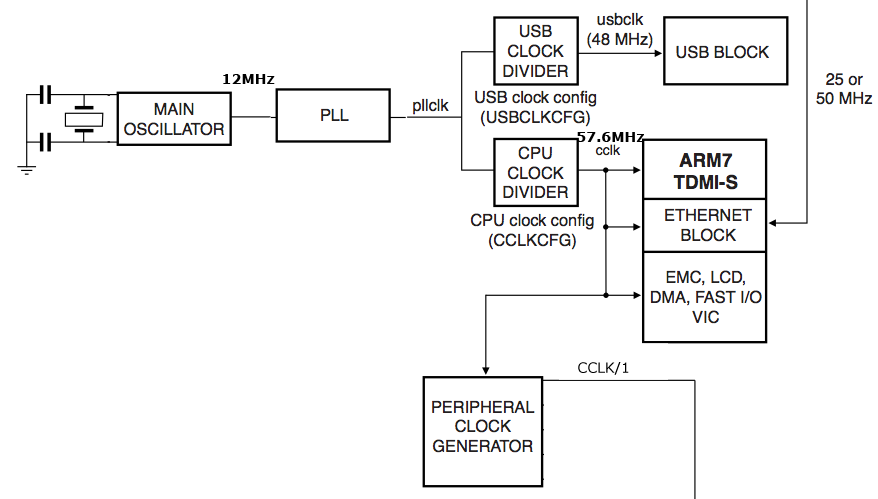
\includegraphics[width=0.7\textwidth]{images/peripheral_clock_gen.png}
		\caption{Peripheral clock to UART}
	\end{centering}
\end{figure}
In order to get the desired clock speed to the UART module, a scale value must be written to the \textit{Divisor Latch Register}.
\\If a baud rate of 9600 is wanted, the value written to the register must be: \\$57.600.000/(16*9600)=375$
\\As seen in the code below, the divisor register is split into two parts (a low and a high part).
\begin{lstlisting}[language=c]
void set_baud(int dev, unsigned int baud){
	switch(dev){
	---
	  case 2:
	    m_reg_write(U2DLL, (((LPC24xx_Fcclk/16)/baud) & 0xFF));
	    m_reg_write(U2DLM, (((LPC24xx_Fcclk/16)/baud) >> 8));
	  break;
	---
	}
}
\end{lstlisting}



The other functions used: \textit{intToStr}, \textit{strToInt}, \textit{chToUpper}, \textit{help} is code reuse from some of the other device drivers provided with the kernel: SFR, ADC and PWM.

%        Implementation
%
%                Mechanical drawings with details explained
%                Electronic diagrams with details explained
%                Source code with details explained
%                Description of integration 
\paragraph{Inserting the UART module in the kernel}
To automatically insert the module in the kernel during startup, a few files shall be made. The first thing to do is to create the different uart files in \/dev and specify that the module shall be inserted to the kernel after startup. The different files created is specified in the rc file. In the kernel folder structure the rc file used is placed in: \textit{/home/emb/uClinux-dist/vendors/EmbeddedArtists/LPC2478OEM\_Board}

\begin{lstlisting}[language=c]
---
/bin/mknod /dev/uart0 c 239 0 
/bin/mknod /dev/uart1 c 239 1
/bin/mknod /dev/uart2 c 239 2
/bin/mknod /dev/uart3 c 239 3
---
if [ -f /drivers/adc.ko ]; then
  insmod /drivers/adc.ko
fi
---
\end{lstlisting}
In the \textit{Makefile} in the same path a line shall be inserted to add the module to the \textit{romfs image} which is extracted during boot time. Also in the top, the value 5 shall be exchanged with 6, to indicate that there is an extra char device.
\begin{lstlisting}[language=c]
---
DEVICES = console,c,6,1
---
$(ROMFSINST) -S drivers/2.6.x/uart/uart.ko /drivers/uart.ko & \
---
\end{lstlisting}
The last thing to do is to add uart to the makefile in the drivers/2.6.x folder, to be sure that the kernel remakes the UART module when compiled if any changed were done. 
\paragraph{Adding the UART user space application}
When compiling a user space application through the kernel, there is no need to specify which gcc compiler to use or which flags to set in the different local Makefiles (this is all set in the big kernel Makefile). Therefore a makefile was found in the uClinux pdf book\footnote{Getting Started With uClinux Development A, page 72} in order to make small changes to the program, add it to the NFS folder and run it on the target, without the need for compiling the whole kernel and restarting the target each time. The makefile used:
\begin{lstlisting}[language=c]
CFLAGS= -Wall -W
LDFLAGS= -Wl,-elf2flt
CC= /usr/local/bin/arm-elf-gcc
RM=rm -f

PROG=uart
SRC= uart.c

OBJ=$(SRC:%.c=%.o)

$(PROG): $(OBJ)
	$(CC) $(CFLAGS) -o $(PROG) $(OBJ) $(LDFLAGS)

.PHONY: clean all dep

clean:
	$(RM) $(PROG) $(OBJ) *~ *.gdb .depend *.elf2flt *.elf
\end{lstlisting}
After finishing the application, it is added to the kernel by following the steps on Klaus wiki\footnote{\url{http://klaus.ede.hih.au.dk/index.php/How-to_add_a_user_space_application_to_uClinux}}.
\subsubsection{Verification}
The module is only verified with the UART2 hardware. The verification of the module is done by the UART user space application. At first the rx and tx pins where short-circuit, to make a loopback. After performing a write to the file by running the UART user space application, the file was read and the values compared to verify that the data was not corrupt. Afterward a test has been made similar to the one performed on the bare-metal driver, where the Embedded Artist board and an MBED communicates with each other through their own power line modules. 
%        Verification
%
%                Module tests
%                Integration tests
%                Acceptance test
\subsubsection{Conclusion}
The UART hardware can be accessed through the device driver, however, the efficiency of the module is not that good. Therefore the driver still need some improvements which shall be further added in order to get a better performance. 
\begin{itemize}
	\item Add interrupts to the receive part, to avoid reading the file once in a while to see if someone wrote anything.
	\item Add file write function, so a whole file can be compressed and sent to another module (wind turbine, photovoltaic, CAES or battery).
	\item Add more flexibility to initializing the module (break control, interrupt, ...) 
	\item Add more error handling and better feedback description if an invalid command is received.
\end{itemize}

%%%%%%%%%%%%%%%%% Dennis End%%%%%%%%%%%%%%%%%%%%%%%%%%%%%%%%%%%
\subsection{Interrupt register - Theis}
The interrupt register is made to tune performance by limiting the number of read statements the ARM7 is doing, in order to read from the Spartan 6. The interrupt register is not by itself fulfilling any requirements, but it is tuning the following: \textit{NF-1.5}\footnote{Requirement is found in table 3.2 in EPRO 3 project energy-hub} and \textit{B-3}\footnote{Requirement is found in table 3.4 in EPRO 3 project energy-hub}
\begin{table}[H]
\centering
	\begin{tabular}{|p{1.2cm}|p{2.3cm}|p{6cm}|p{6cm}|}
	\hline
	ID		& Requirement		& Description																& Comments\\\hline
	NF-1.5	& HW Interface		& 1 start button for the hub. 10 buttons to each start a module.			& It is only reading if the buttons state changes\\\hline
	B-3		& Errors			& Humidity and Temperature sensor will be placed inside the system housing	& The Spartan 6 interrupts if one of the following is happening\\\hline
	B-3.1	& Humidity			& If the humidity is above the maximum level 70\%, the system shuts down	& ARM7 only read on interrupt\\\hline
	B-3.2	& Temperature High	& If the temperature is higher than 55 degrees, the system shuts down		& ARM7 only read on interrupt\\\hline
	B-3.3	& Temperature Low	& If the temperature is below 0 degrees, the system shuts down				& ARM7 only read on interrupt\\\hline
	\end{tabular}
\end{table}
%			Intro
%					verification specification
%					deployment specification
\subsubsection{Analysis}
The purpose of the interrupt register is to limiting the number of readings the ARM7 is making from the Spartan 6. There is one interrupt pin routed from the AMR7 to the Spartan 6, but there is two blocks in the Spartan 6 that makes data for the ARM7. These blocks are the switch input block and the analog to digital converter\footnote{ADC} block. One way to use the interrupt is to allow the switch block to interrupt when a user interact with the system, and then read the ADC with a specific time interval. But to avoid to many unnecessary readings of the ADC, the interrupt register is the only block that is allow to interrupt the ARM7, the interrupt register gets interrupt signals from the ADC and the switch blocks, the register is arranging the interrupt, and when the ARM7 is interrupted, it reads data from the register to find out which block it should read.
\begin{figure}[H]
	\begin{centering}
		%\missingfigure{Updated timebox figure}
		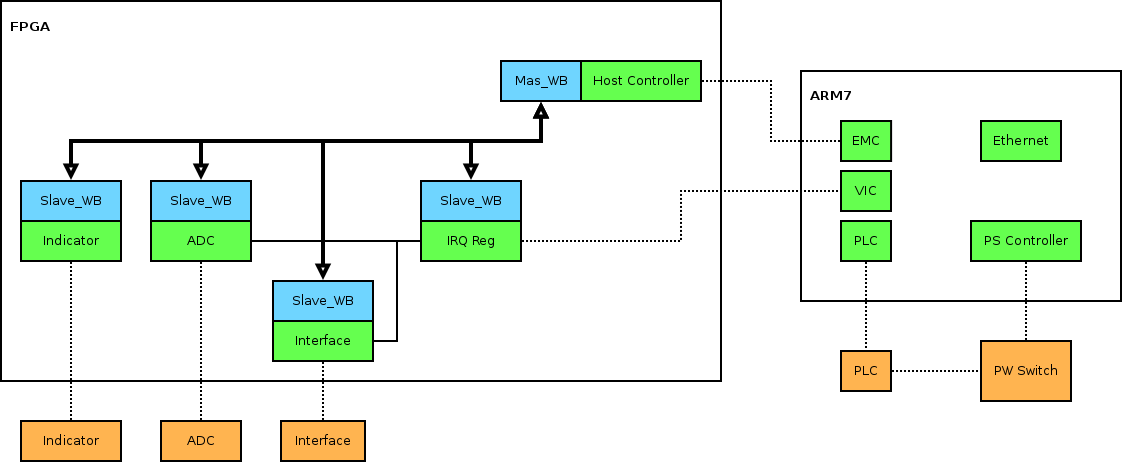
\includegraphics[width=1.0\textwidth]{images/tb5_modules_design.png}
		\caption{Module design with IRQ register}
	\end{centering}
\end{figure}
When a block sends an interrupt to the IRQ\footnote{Interrupt Request} register, it locates the interrupt and put the address to the block on to a FIFO\footnote{First In First Out}, and sends an interrupt to the ARM7, then the AMR7 read the FIFO to get the address on the interrupting block, in that way the ARM7 knows where to read next.
%			Analysis
%
%                Refactored block diagram
%                Refactored class diagram
%                Detailed use cases
%                User interface specification
%                System interface specification
%                Dimensioning specification 
%
\subsubsection{Design}
The purpose of the interrupt register is to make interrupt functionality on several block with only one interrupt pin to the ARM7. The interrupt register shall be optimized to wishbone use. The interrupt register without wishbone has the inputs, a vector of size N\footnote{N = number of blocks that is allow to interrupt} and N AddrRange\footnote{Wishbone address range} bit wide vectors for the interrupt data. The output is the IRQ pin to the ARM7 and a data vector equal to the wishbone data width. This is shown in the figure below.
\begin{figure}[H]
	\begin{centering}
		%\missingfigure{Updated timebox figure}
		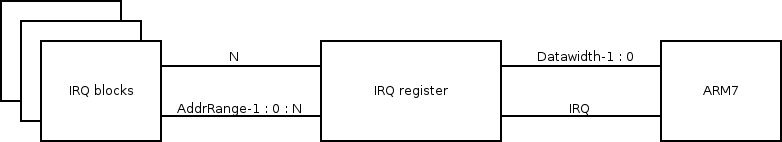
\includegraphics[width=1.0\textwidth]{images/tb5_irq_reg_nowb.png}
		\caption{IRQ register without wishbone}
	\end{centering}
\end{figure}
When a block needs to make an interrupt, it puts the wishbone address onto the input array to the IRQ register, and then sets the interrupt output high to tell the IRQ register that there is a valid address that needs to be read. The IRQ register save the address and interrupt the ARM7. When an interrupt occurs on the ARM7, it read the IRQ register to get the address that it shall read next, in this way it takes two wishbone read cycles for the ARM7 to get the right data, but the ARM7 is only reading if the Spartan 6 have valid data to read, instead of make reading with specific interval. The IRQ register save the interrupt in a FIFO in case interrupt is made faster than the ARM7 can read.\\
\paragraph{Interrupt output}
The interrupt output is set low as long a the FIFO is not empty, to tell the ARM7 to keep on reading till the FIFO is empty and sets the IRQ high again.
\paragraph{Data output}
The data output is equal to the wishbone data width, in this case it is 16 bit, and the address is 7 bit. The seven lowest data bits is used for the address to the block that sends the interrupt, the rest of the bits can be used for extra data from the IRQ register.
\begin{figure}[H]
	\begin{centering}
		%\missingfigure{Updated timebox figure}
		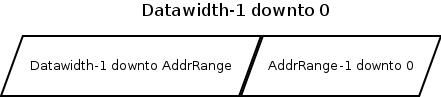
\includegraphics[width=0.55\textwidth]{images/tb5_irq_reg_data_o.png}
		\caption{IRQ register data output}
	\end{centering}
\end{figure}
%        Design
%
%                UML/SysML deployment view(s)
%                Mechanical specifications and dimensioning
%                HW module specification per block
%                UML SW deployment view
%                Class specification
%                Refactored class diagram½
%                Use case scenarios specifications
%                Sequence diagrams
%
\subsubsection{Implementation}
A block diagram for the interrupt register is shown below. It consist of three block for handling the interrupt, a input block which handled the input and write data to the FIFO. The FIFO act like memory for the interrupt data, and sends a interrupt to the ARM7. The output block takes input from the wishbone and handle the data to the wishbone, form the FIFO.
\begin{figure}[H]
	\begin{centering}
		%\missingfigure{Updated timebox figure}
		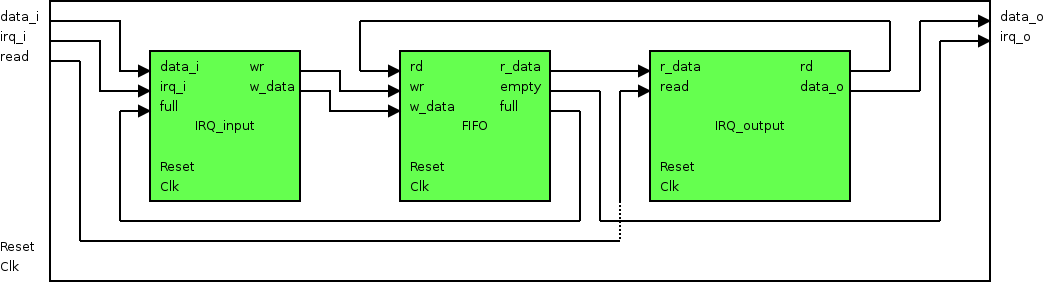
\includegraphics[width=1\textwidth]{images/irq_reg_block_dia.png}
		\caption{Block diagram for the IRQ register}
	\end{centering}
\end{figure}

\paragraph{FIFO - First In First Out}
The FIFO buffer is where the interrupt data is stored before they are read. The input block write data into it, and the output block read data out of it. The FIFO is necessary if the Spartan6 make interrupt faster than the ARM7 can read them. The figure below shows how the First In First Out principle is working.
\begin{figure}[H]
	\begin{centering}
		%\missingfigure{Updated timebox figure}
		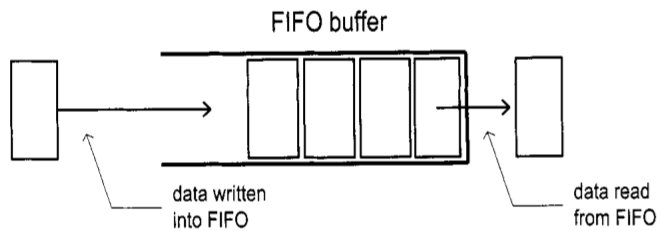
\includegraphics[width=0.6\textwidth]{images/tb5_fifo.png}
		\caption{Conceptual diagram of a FIFO buffer}
	\end{centering}
\end{figure}
The FIFO buffer code is from the book \textit{FPGA Prototyping by VHDL Examples - Listing 4.20}. It is a standard FIFO buffer, with a data vector input, an input for read and one for write, plus clock and reset. As output there is a data vector equal to the input vector, further more there is an empty and a full signal to indicate if the buffer is empty or full. A block diagram for the FIFO buffer is shown below.
\begin{figure}[H]
	\begin{centering}
		%\missingfigure{Updated timebox figure}
		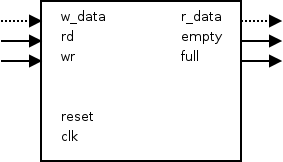
\includegraphics[width=0.45\textwidth]{images/tb5_fifo_block.png}
		\caption{State diagram for input}
	\end{centering}
\end{figure}
The FIFO buffer is used to hold the interrupt data from the other blocks in order to present it for the ARM7 in the right order. A digram of how it works is shown below.
\begin{figure}[H]
	\begin{centering}
		%\missingfigure{Updated timebox figure}
		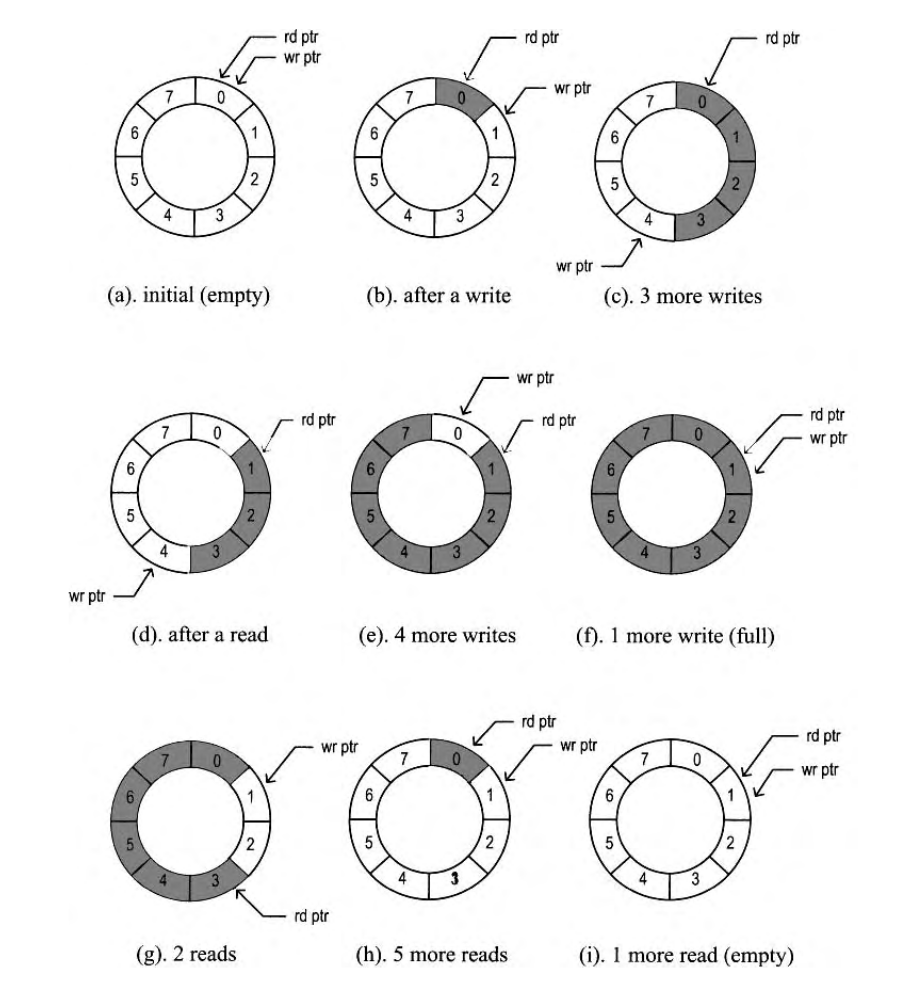
\includegraphics[width=1.0\textwidth]{images/tb5_fifo_ring.png}
		\caption{Ring buffer diagram}
	\end{centering}
\end{figure}
A ring buffer writes data in at the write pointer and count it up by one. When a read state happens it reads from the read pointer and count it up by one. this is also way a full and empty signal i necessary, in order not to overwrite data or read ahead of the write pointer.

\paragraph{IRQ input}
The input block gets data and interrupt input from every block with interrupt permissions in the system. The purpose of the block is to handle which block is interrupting and which data that have to be written to the FIFO in order to be handle by the ARM7 in the right way. Below the state diagram of the input block is shown. The purpose of a state digram is to make the coding easier.\\
When in IDLE the FIFO write is set low, the interrupt inputs is check, if non of them is high the interrupt counter is set low, to enable new interrupts. If a interrupt is high the state is change to IRQx, where the data output to the FIFO is set to the data from the interrupting source, after that is checks if it is the first time this data is written to the FIFO, if that is the case, the data is written to the FIFO and the returns to IDLE. 
\begin{figure}[H]
	\begin{centering}
		%\missingfigure{Updated timebox figure}
		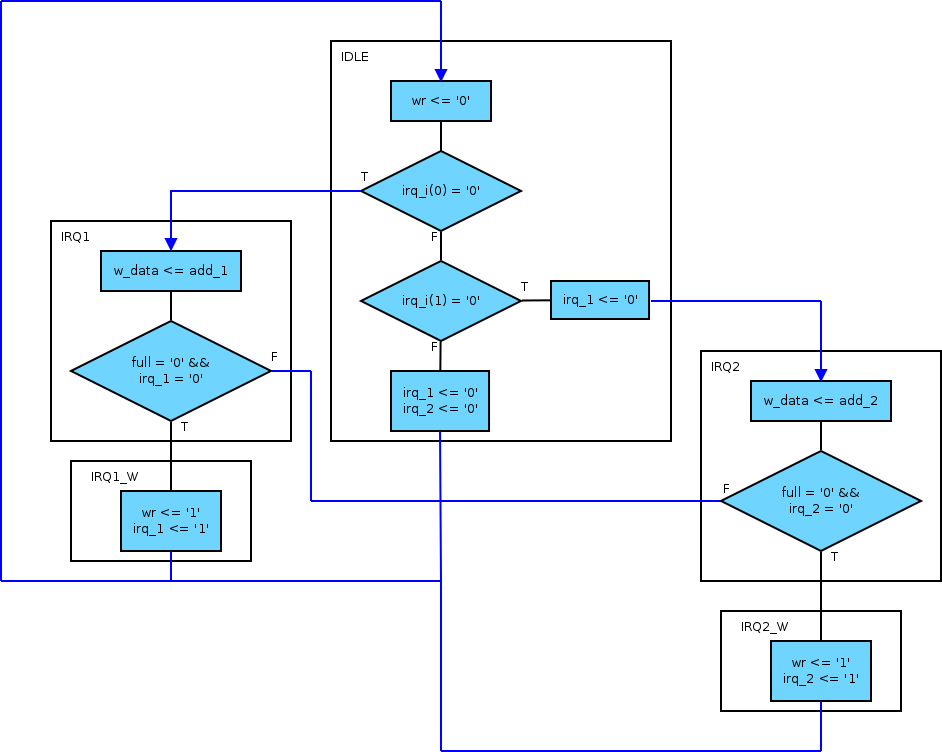
\includegraphics[width=0.9\textwidth]{images/tb5_irq_input_state.png}
		\caption{State diagram for input}
	\end{centering}
\end{figure}
In the code below the states are defined, this is easily done from the state diagram, the signals that can have the different states a value is also defined here.
\begin{lstlisting}[language=VHDL]
...
	--Types
	type state_type is	(
								IDLE,
								IRQ1,
								IRQ1_W,
								IRQ2,
								IRQ2_W
								);
	--Signals
	signal state_reg		: state_type;
	signal state_next		: state_type;
	signal irq_1				: std_logic		:=	'0';
	signal irq_2				: std_logic		:=	'0';
...
\end{lstlisting}
This code is where the states are set, if reset is active the state is set to IDLE else the state is set to state\_next.
\begin{lstlisting}[language=VHDL]
...
	-- state register
	process(Clk, Reset)
	begin
		if	(reset = '1') then
			state_reg		<= IDLE;
		elsif (Clk'event and Clk='1') then
			state_reg		<= state_next;
		end if;
	end process;
...
\end{lstlisting}
This is the part of the code where the state digram is implemented. A case statement is made with the state value as input. First the IDLE state is defined, here wr is set low, then it check if there is a interrupt, if that is the case then it sets the state to IRQx which sets the data and then check if it is first time the data is written else it just sets the state to IDLE, if it is first time the state is set to IRQx\_W where it write the data into the FIFO.
\begin{lstlisting}[language=VHDL]
...
	-- next state/output logic
	process(state_reg, irq_i, add_1, add_2, full, irq_1, irq_2)
	begin
		state_next		<= state_reg;
		--wr					<= '0';
		case state_reg is
		-- Idle state -------------------------------------------
			when IDLE =>
				wr		<= '0';
				if(irq_i(0) = '1') then
					state_next		<= IRQ1;
				elsif(irq_i(1) = '1') then
					irq_1					<= '0';
					state_next		<= IRQ2;
				else
					irq_1		<= '0';
					irq_2		<= '0';
				end if;
		-- IRQ1 state -------------------------------------------
			when IRQ1 =>
				w_data				<= add_1;
				state_next		<= IRQ1_W;

			when IRQ1_W =>

				state_next		<= IDLE;
				if((not full and not irq_1) = '1') then
					wr			<= '1';
					irq_1		<= '1';
				end if;
		-- IRQ2 state -------------------------------------------
			when IRQ2 =>
				w_data				<= add_2;
				state_next		<= IRQ2_W;

			when IRQ2_W =>

				state_next		<= IDLE;
				if((not full and not irq_2) = '1') then
					wr			<= '1';
					irq_2		<= '1';
				end if;
		end case;
	end process;
...
\end{lstlisting}

\paragraph{IRQ output}
The output block is reading the data out of the FIFO and present them for the wishbone. It gets a read input from the wishbone, when the ARM7 wants to read data from the register. The main purpose of the block is to make sure that the wishbone read the write data, and it is only reading once from the FIFO.\\
A state diagram for the output block is shown below. In the IDLE state rd is set low, then et check if the wishbone wants to read, else it reset the read counter, if the wishbone wants to read, the IDLE state checks if it is the first time by checking the read counter, if it is the first time the rd is set high to get the next data from the FIFO, and the read counter is set to one.
\begin{figure}[H]
	\begin{centering}
		%\missingfigure{Updated timebox figure}
		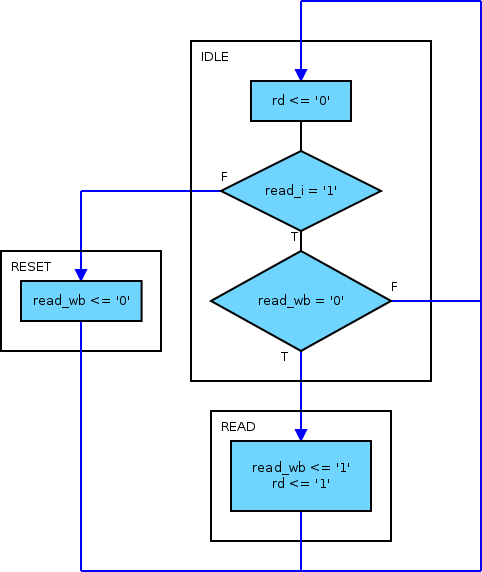
\includegraphics[width=0.55\textwidth]{images/tb5_irq_output_state.png}
		\caption{State diagram for output}
	\end{centering}
\end{figure}
Here the states is defined plus the read counter.
\begin{lstlisting}[language=VHDL]
...
	--Types
	type state_type is	(
											IDLE,
											READ_O,
											RSET
											);
	--Signals
	signal state_reg		: state_type;
	signal state_next		: state_type;
	signal read_wb			: std_logic;
...
\end{lstlisting}
The lower bits in the data\_o is set to the data from the FIFO, the other bits is set to zero. In the process the next state is loaded.
\begin{lstlisting}[language=VHDL]
...
	data_o(Datawidth-1 downto AddrRange)	<= (others => '0');
	data_o(AddrRange-1 downto 0)					<= r_data;

	-- state register
	process(Clk, Reset)
	begin
		if	(reset = '1') then
			state_reg		<= IDLE;
		elsif (Clk'event and Clk='1') then
			state_reg		<= state_next;
		end if;
	end process;
...
\end{lstlisting}
Below the state actions is defined following the state diagram. The rd is set low in IDLE and the wishbone read is checked. In READ the read counter is set to one and rd is set high to read data out of the FIFO.
\begin{lstlisting}[language=VHDL]
...
	-- next state/output logic
	process(state_reg, read_i, r_data, read_wb)
	begin
		state_next	<= state_reg;
		rd					<= '0';
		read_wb			<= read_wb;
		case state_reg is
		-- Idle state -----------------------------------------------------
			when IDLE =>
				rd		<= '0';
				if	(read_i = '1') then
					if	(read_wb = '0') then
						state_next		<= READ_O;
					else
						state_next		<= IDLE;
					end if;
				else
					state_next		<= RSET;
				end if;
		-- READ_O state ---------------------------------------------------
			when READ_O =>
				state_next		<= IDLE;
				read_wb				<= '1';
				rd						<= '1';
		-- RSET state -----------------------------------------------------
			when RSET =>
				state_next	<= IDLE;
				read_wb			<= '0';
		end case;
	end process;
...
\end{lstlisting}

\paragraph{Wishbone interface}
In order to use the interrupt register in the system, is shall be implemented as a wishbone slave, with a wishbone interface, this is done in the code below. The error and retry bit i set to zero, the acknowledge bit i set then the strobe input and the cycle input is high. In the process a synchronous reset is made. If the reset is inactive, it checks if the strobe and cycle input is high and the write enable is low, the meaning is to check if the wishbone wants to read or write. This module is a read only so it is not reacting on a write statement. If the wishbone wants to read, the data output is set and a read to the output block is set high, when the wishbone determinates the read cycle the data output is set to zero and the read statement for the output block is set low again.
\begin{lstlisting}[language=VHDL]
...
-- =================================================
-- WishBone logic
-- =================================================
	--  Concurrent assignments
	--	Wishbone cycle acknowledge
	err_o <= '0';	--error signal
	rty_o <= '0';	--retry signal
	ack_o <= stb_i and cyc_i;  --! asynchronous cycle termination is OK here.
	--Wishbone read
	data_output	:	process(clk_i)
	begin
		if(clk_i'event and clk_i = '1') then
			if(rst_i = '1') then
				dat_o <= (others => '0');
			else
				if((cyc_i and stb_i and not we_i) = '1') then
					case adr_i is
						when WBS_REG1 =>
							dat_o		<= data_o;
							read_i	<= '1';
						when others =>
					end case;
				else
				dat_o		<= (others => '0');
				read_i	<= '0';
				end if;
			end if;
		end if;			
	end process;
...
\end{lstlisting}
%        Implementation
%
%                Mechanical drawings with details explained
%                Electronic diagrams with details explained
%                Source code with details explained
%                Description of integration 
%
\subsubsection{Verification}
The verification of the IRQ register is made in a VHDL test bench, because there is currently no blocks with interrupt ability implemented. The verification test bench is shown below. The test is made by make four interrupts, this can be seen on the \textit{IRQ\_in} signal which has four pulses on the two signals. The address on \textit{add\_1} and \textit{add\_2} is written into the FIFO. The test bench also shows that the \textit{IRQ\_out} change after the first interrupt is assigned. After this four wishbone reads are made, by setting the cycle and the strobe input high, this give a acknowledge bit, and the \textit{Data\_out} is change to the first element in the FIFO, and the next read get the next data and further on. After the last wishbone read the FIFO is empty and the \textit{IRQ\_out} is set high again to indicate there is no interrupt.
\begin{figure}[H]
	\begin{centering}
		%\missingfigure{Updated timebox figure}
		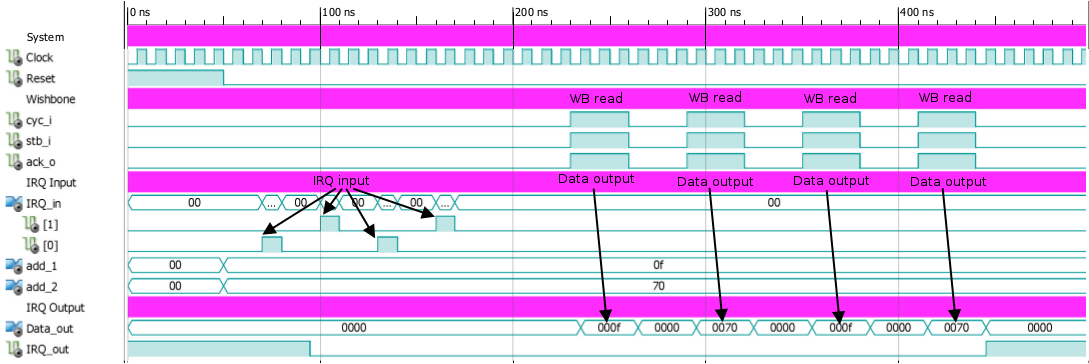
\includegraphics[width=1.0\textwidth]{images/tb5_irq_reg_testbench1.png}
		\caption{Test bench for the interrupt register}
	\end{centering}
\end{figure}
%        Verification
%
%                Module tests
%                Integration tests
%                Acceptance test
\subsubsection{Conclusion}
The test bench verify that the interrupt register is working with virtual signals in simulation. The switch block is to be change to have interrupt ability, and then it shall be implemented with the interrupt register and tested properly with communication and interrupt to the ARM7


\subsection{Deployment}
\paragraph{UART Device Driver}
The first version of the Device Driver is up and running (v0.1), which has implemented read and write functionality (non interruptible). Also different write calls have been implemented in order to initialize a channel.
\paragraph{Power Switch}
The power switch system is under development, 4 of this modules will be developed and a test bench build using fast prototyping tools. In time box 6 the complete development of this main system will be finish and a prototype will be present to the client.
	%which versions of the prototype the customer will get
	%with what functionality.
\paragraph{Interrupt register}
The interrupt register works in a test bench with wishbone interface. The implementation in the Spartan 6 is the next step and, interrupt ability is to be added to the switch block.
	%which versions of the prototype the customer will get
	%with what functionality.\newpage
%% % % % % % % % % % % % % % % % % % % % % % % % % % % % % % % % % % % % % % % % %
% INTRO
% % % % % % % % % % % % % % % % % % % % % % % % % % % % % % % % % % % % % % % % %
\section{Time box 6}
%\listoftodos
\subsection{Time box planning}

\begin{figure}[H]
	\begin{centering}
		\missingfigure{Updated timebox figure}
		%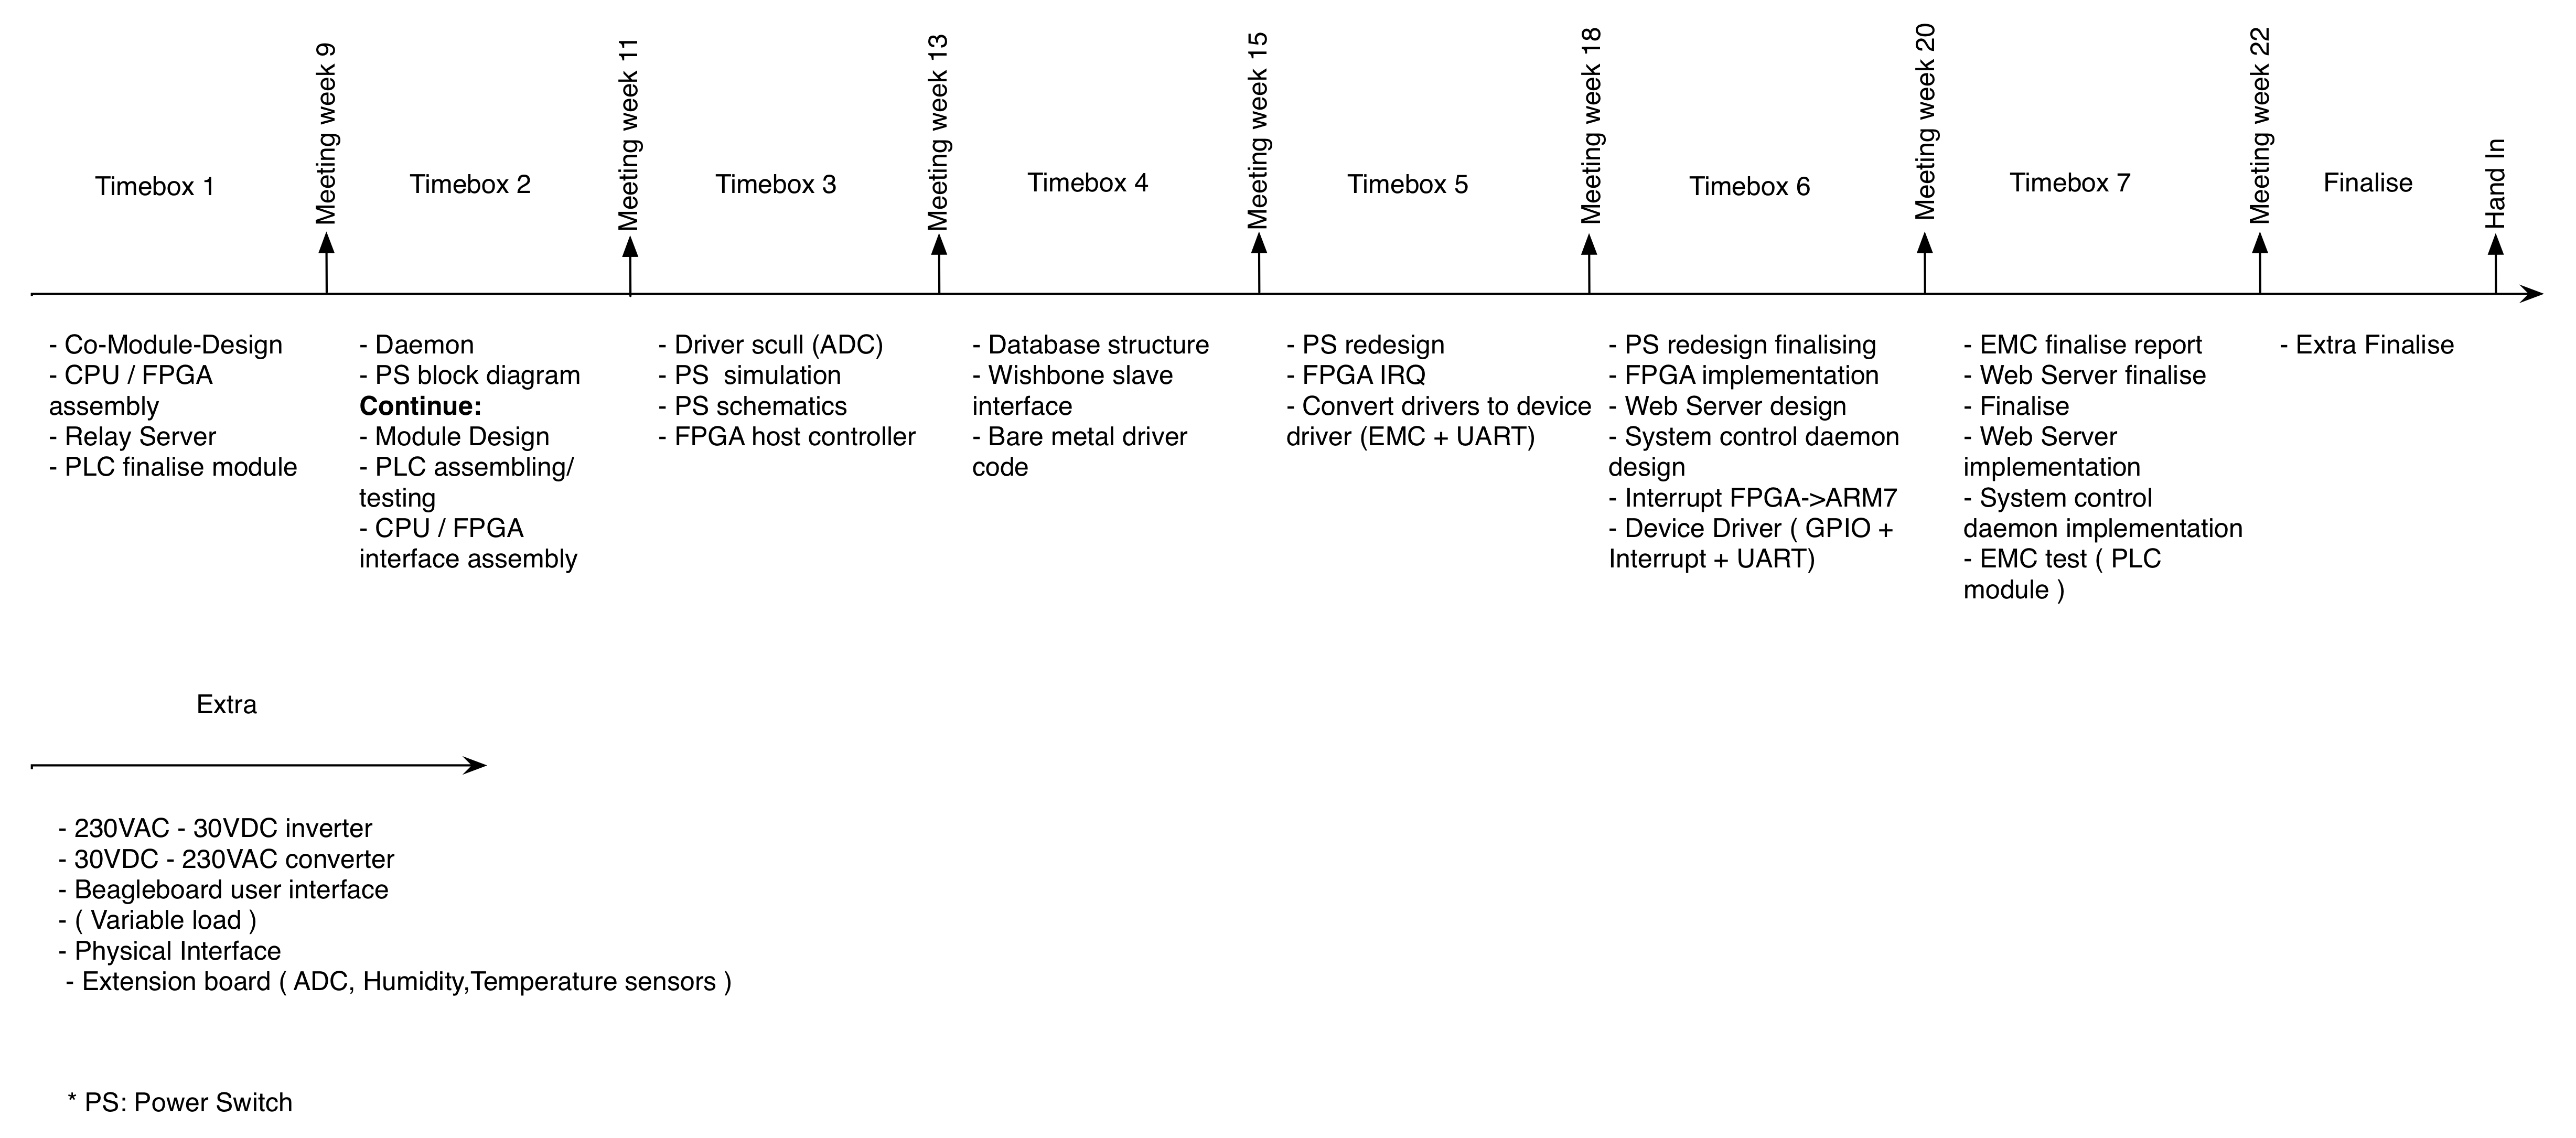
\includegraphics[width=1.0\textwidth]{images/tb_r5.png}
		%\caption{Updated time-box}
	\end{centering}
\end{figure}

\subsubsection{Work to be done in this time box}
\todo[inline]{Update List}
\begin{itemize}
	\item Switch interrupt
	\begin{itemize}
		\item debouncer
		\item Interrupt
	\end{itemize}
	\item Web Server
		\begin{itemize}
			\item Web Services - Communication
			\item File structure
		\end{itemize}
	\item UART Device driver
	\begin{itemize}
		\item Improvement on the driver made in last timebox
	\end{itemize}
\end{itemize}

\paragraph{Description:}
%\todo[inline]{Update Description}
\begin{description}
	\item[Switch interrupt] In order to send data to the interrupt register, an interrupt output for the switch block has to be implemented, and the switches has to be debounced, to secure that the interrupt data is send only once.
	\item[Web Server] The web server is the communication between the system and the world. The communication between the web server and energy hub is implemented and the file structure is set for the collaboration of other teams/modules.
	\item[UART Device driver] Implementation of input/output control and interrupt handling in the UART device driver made in time box 5.
\end{description}

\subsubsection{Time planning}

\begin{table}[H]
\centering
%	\todo[inline]{Update Time}
	\begin{tabular}{|l|c|c|c|c|c|}
		\hline
		~			& Switch interrupt		& Jesus thing		& UART improvements	\\ \hline
		Estimation	& 12					& 15				& 5					\\
		Actual		& 20					& 22				& 17				\\
		Developer	& Theis					& Paulo			& Dennis				\\
		\hline
	\end{tabular}
	\caption{Estimation and actual time used on the project}
\end{table}

% % % % % % % % % % % % % % % % % % % % % % % % % % % % % % % % % % % % % % % % %
% % % % % % % % % % % % % % % % % % % % % % % % % % % % % % % % % % % % % % % % %
% Scaling the project due to limited time.
% % % % % % % % % % % % % % % % % % % % % % % % % % % % % % % % % % % % % % % % %
\subsection{Project scaling}
Unfortunately there is still a lot of work tasks to be done before the fully project is realized. With only 2 weeks before delivering the report it has been decided to down scale the project, to have some blocks fully up and running. The picture below shows the parts that will hopefully be implemented in the handed in version. 
\begin{figure}[H]
	\begin{centering}
		%\missingfigure{Updated timebox figure}
		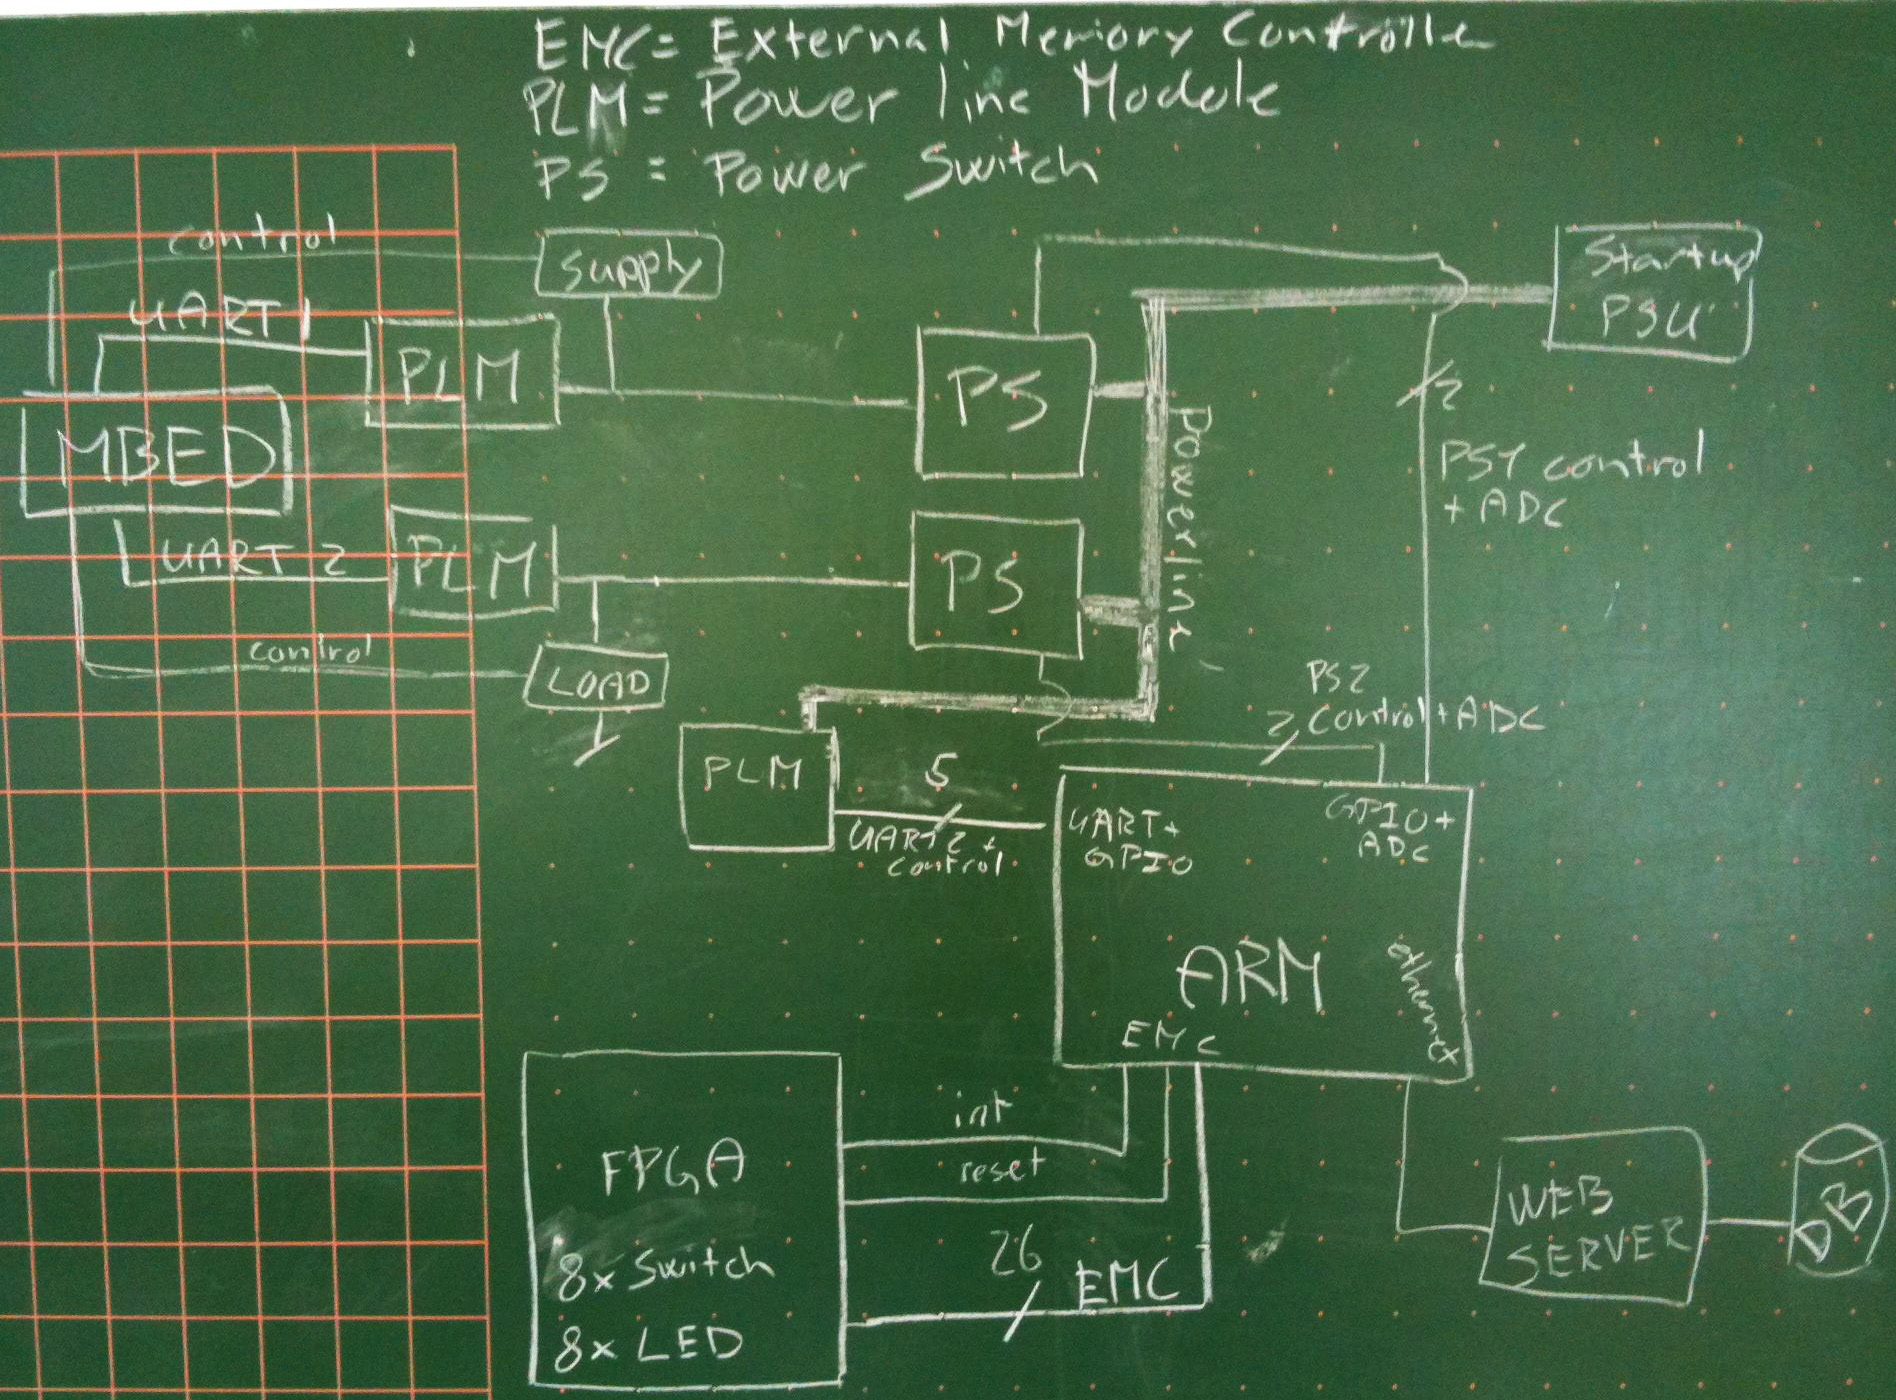
\includegraphics[width=1.0\textwidth]{images/project_scaling_tb6.jpg}
		\caption{Project Scaling diagram}
	\end{centering}
\end{figure}
\textbf{The scaled project will then contain:} 
\begin{itemize}
	\item ARM to FPGA communication through External Memory Controller. The ARM gets an interrupt from the FPGA whenever a switch changes status. The ARM then sets the LEDS on the ARM board according to the switches status.
	\item UART communication to Power Line Module to send and transmit data between two modules. 
	\item MBED setup to work as two modules (communicating with the ARM board through two power line modules).
	\item Dummy protocol to send data from MBED to ARM board. 
	\item Direct received data from MBED to WEB-server.
	\item \todo[inline]{JESUS, something about database and web server}
	\item ...
\end{itemize} 
The setup will then be able to check which state it should be running in, according to the switches set on the FPGA board. The ARM board will be able to control the Power Line modules (switching direction and turning off modules). When communication is established between the MBED and the ARM through Power Line, the data received from the MBED is verified and sent to the WEB-server. 
\todo[inline]{JESUS, something about database and web server}

% % % % % % % % % % % % % % % % % % % % % % % % % % % % % % % % % % % % % % % % %
% % % % % % % % % % % % % % % % % % % % % % % % % % % % % % % % % % % % % % % % %
% Theis Thing
% % % % % % % % % % % % % % % % % % % % % % % % % % % % % % % % % % % % % % % % %
\subsection{Switch interrupt - Theis}
%			Intro
%					verification specification
%					deployment specification
%
This part is, together with the interrupt register from earlier timebox a way to tune performance in reading and writing between the Spartan 6 and the LPC2478.
\subsubsection{Analysis}
%			Analysis
%
%                Refactored block diagram
%                Refactored class diagram
%                Detailed use cases
%                User interface specification
%                System interface specification
%                Dimensioning specification 
%
The interrupt block in the Spartan 6 is the switch block. The switch block needs to be redesign in order to get an interrupt output to the interrupt register, the switches also needs to be debounced, to prevent it from sending the same interrupt data more than once. Two output is added to the switch block, one single bit for interrupt indication and a 7 bit vector for the data to the interrupt register. Inside the block a finite state machine is made for denouncing the switches. Below the redesigned switch block is shown.

\begin{figure}[H]
	\begin{centering}
		%\missingfigure{Updated timebox figure}
		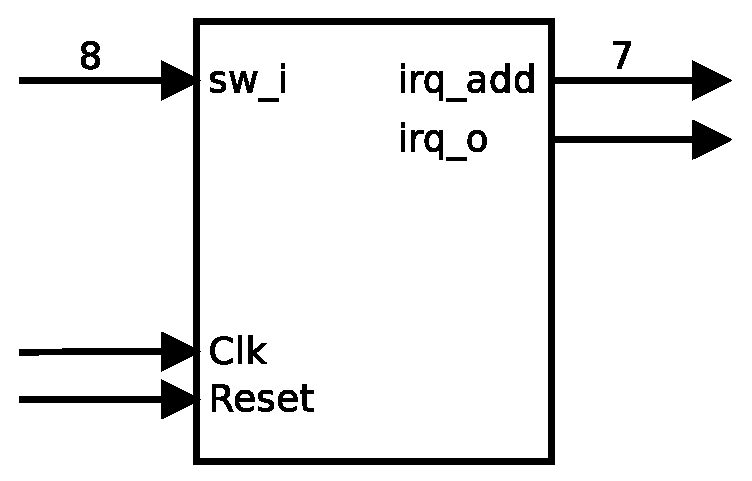
\includegraphics[width=0.3\textwidth]{images/tb6_switchblock.eps}
		\caption{Updated switch block}
	\end{centering}
\end{figure}


\subsubsection{Design}
%       	 Design
%
%                UML/SysML deployment view(s)
%                Mechanical specifications and dimensioning
%                HW module specification per block
%                UML SW deployment view
%                Class specification
%                Refactored class diagram
%                Use case scenarios specifications
%                Sequence diagrams
%
Because of switch bounce, the block needs to take care of this. Below a picture of switch bouncing is shown. The problem is every time the signal goes high the switch block will send data to the interrupt register, to prevent this the block compare a delayed input signal to the present signal, and first when the signal is stable, the system will react on the input.

\begin{figure}[H]
	\begin{centering}
		%\missingfigure{Updated timebox figure}
		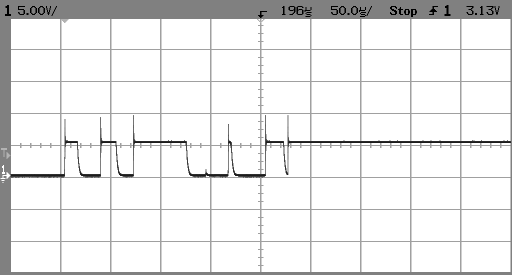
\includegraphics[width=0.5\textwidth]{images/tb6_bounce.png}
		\caption{Switch bouncing}
	\end{centering}
\end{figure}

To debounce the switch a state machine for the switch block is made. This diagram is shown below. The start box set the start output signal to the input signal. The interrupt signal is set high in the OUT0 state, and low again in the IDLE state after the "q2" delay. This is done to have the interrupt signal high enough time for the interrupt register to save the data. The "q1" delay is used to compare the input signal with the output signal in order to capture changes on the 8 switches.

\begin{figure}[H]
	\begin{centering}
		%\missingfigure{Updated timebox figure}
		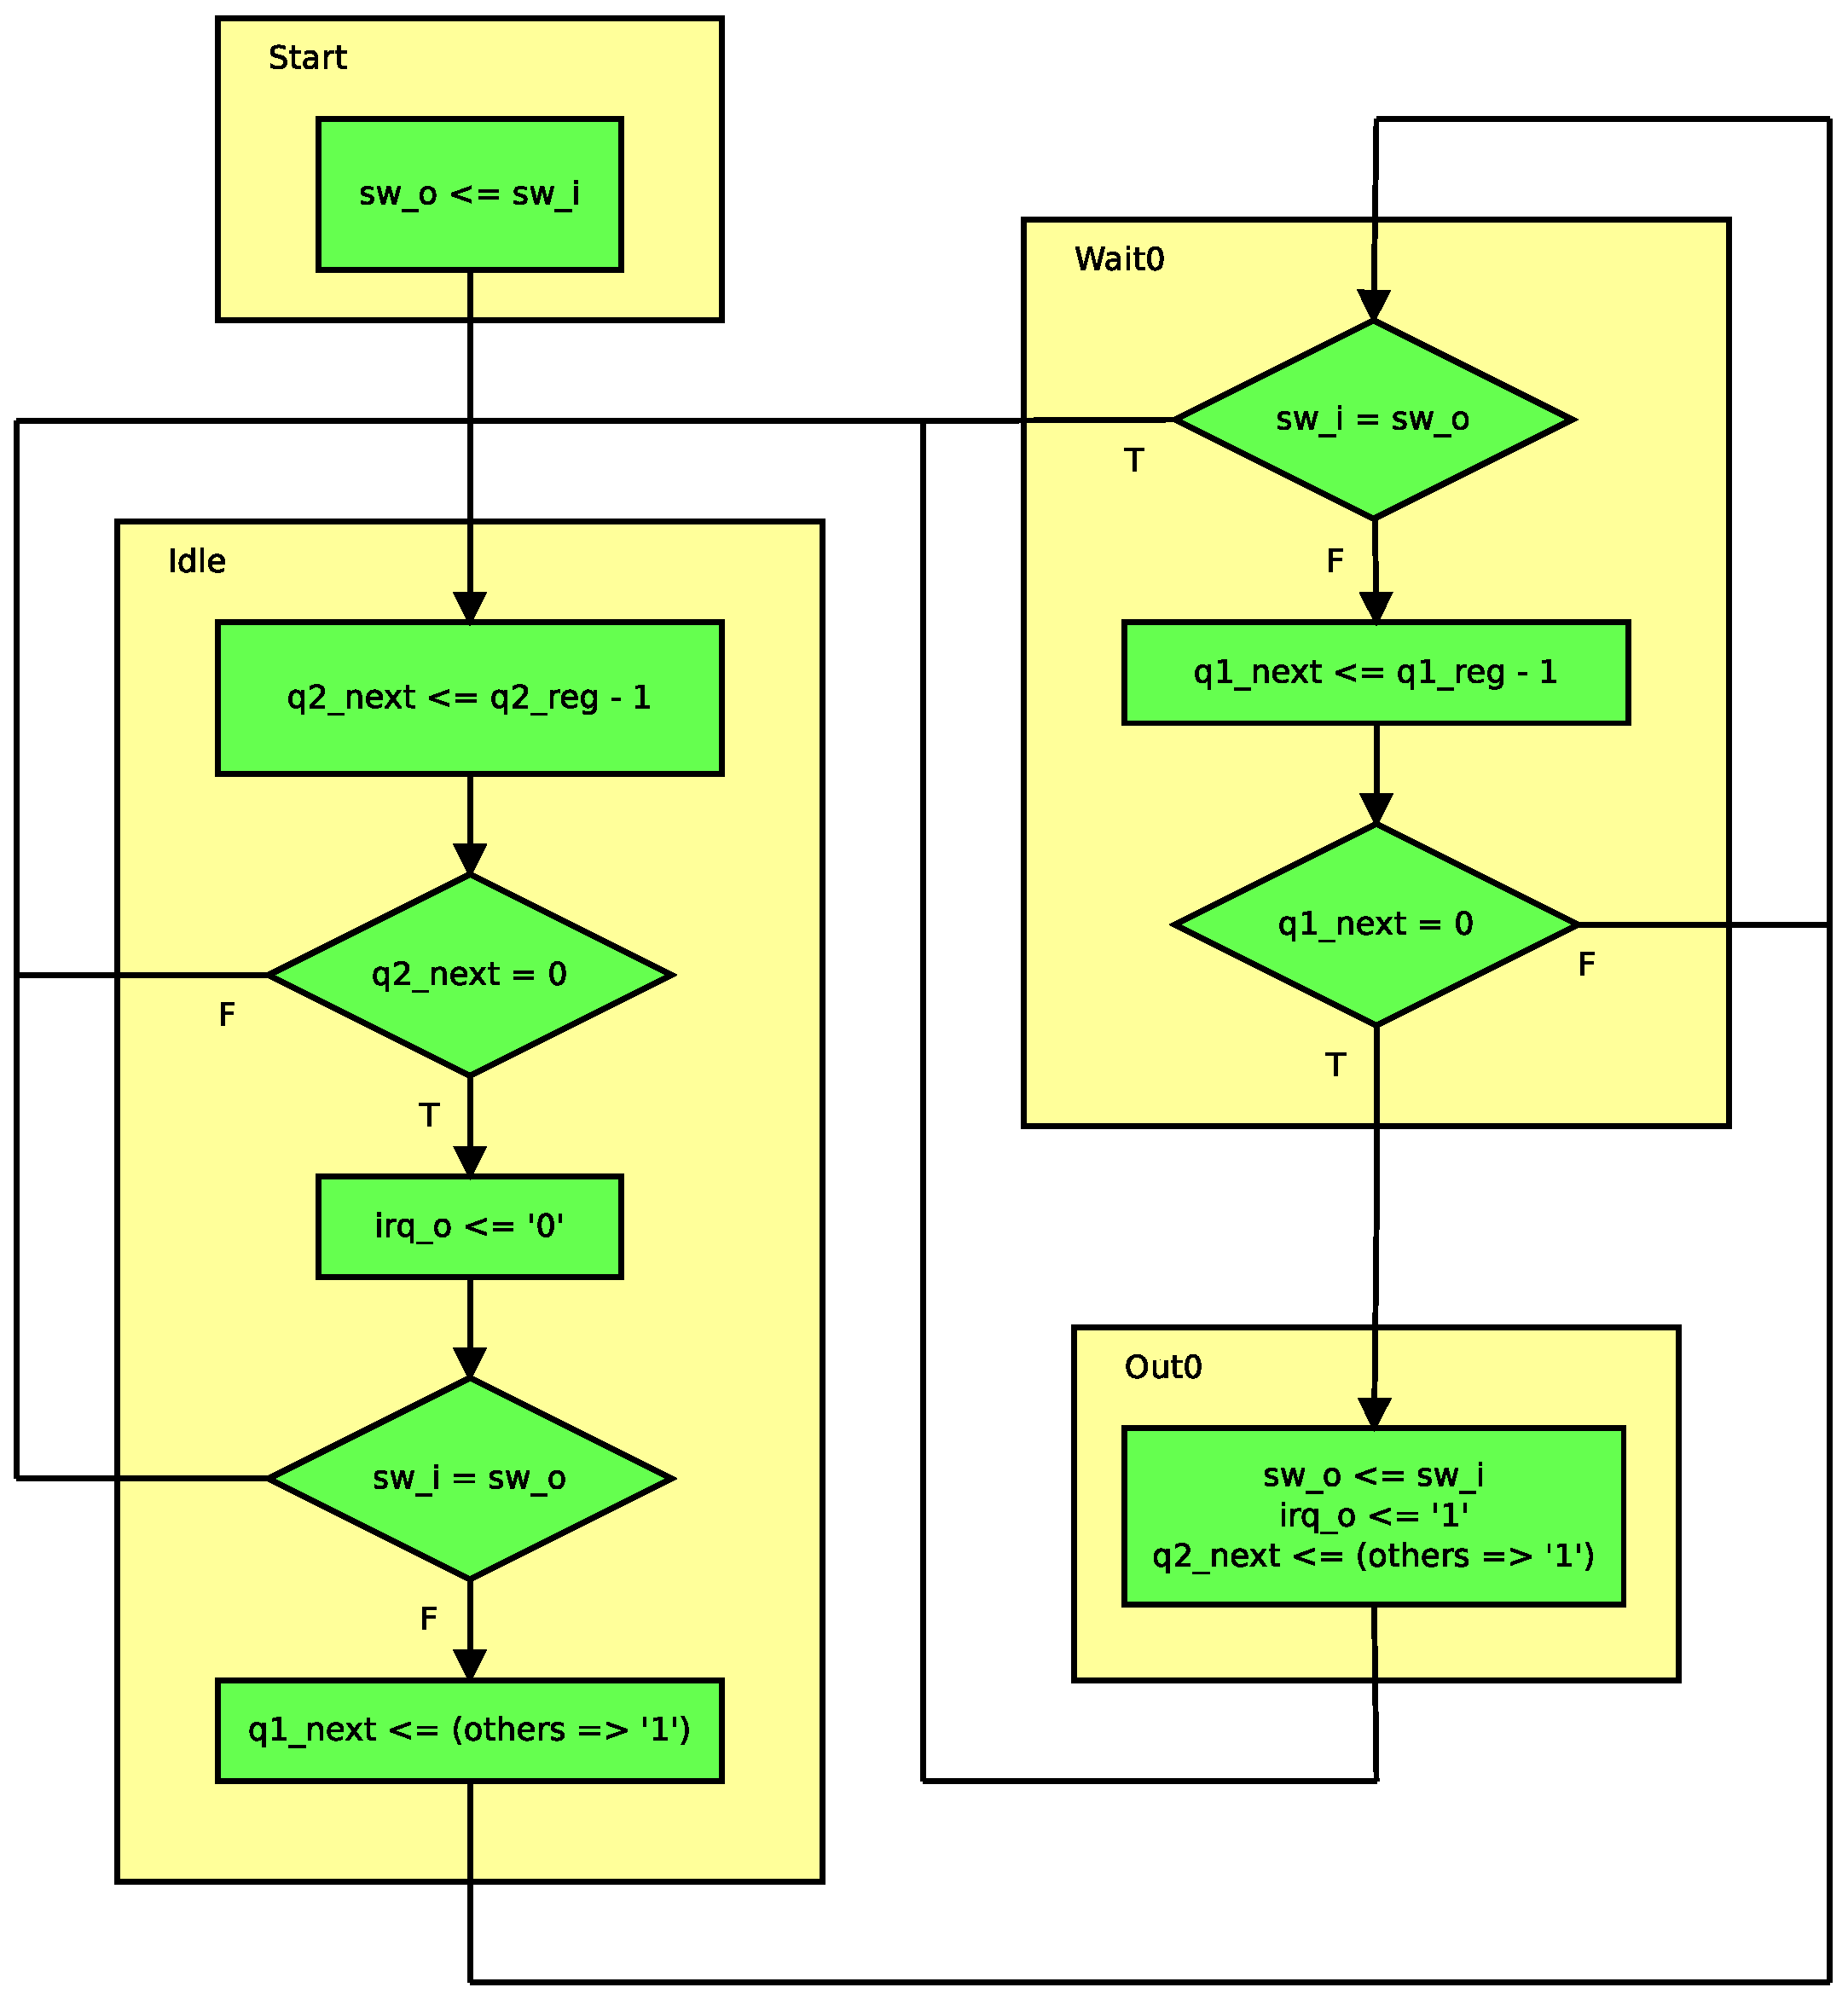
\includegraphics[width=0.7\textwidth]{images/tb6_switch_FSD.eps}
		\caption{Switch block state machine}
	\end{centering}
\end{figure}

\subsubsection{Implementation}
%     	   Implementation
%
%                Mechanical drawings with details explained
%                Electronic diagrams with details explained
%                Source code with details explained
%                Description of integration 
%
The code for the IDLE state is shown below, here the "q2" delay is used in the start, then the interrupt pin is set to zero, then the input and output is compared, if they are not equal the next state is WAIT0 and the "q1" delay is set.
\begin{lstlisting}[language=VHDL]
...
when IDLE =>
	q2_next <= q2_reg-1;
	if	(q2_next = 0) then
		irq_o <= '0';
		if	(sw_i = sw_o) then
			state_next <= IDLE;
		else
			q1_next		<= (others => '1');
			state_next	<= WAIT0;
		end if;
	else
		state_next <= IDLE;
	end if;
...
\end{lstlisting}
In the WAIT0 state the input and output is compared repeatedly to check if the input is stable. If the input is stable long enough time the OUT0 state is entered.
\begin{lstlisting}[language=VHDL]
...
when WAIT0 =>
	if	(sw_i = sw_o) then
		state_next <= IDLE;
	else
		q1_next <= q1_reg-1;
		if	(q1_next = 0) then
			state_next <= OUT0;
		else
			state_next <= WAIT0;
		end if;
	end if;
...
\end{lstlisting}
In the OUT0 state the switch output is set to switch input signal, and an interrupt signal is set high, the "q2" delay is set and it returns to the IDLE state.
\begin{lstlisting}[language=VHDL]
...
when OUT0 =>
	sw_o		<= sw_i;
	irq_o		<= '1';
	q2_next		<= (others => '1');
	state_next	<= IDLE;
...
\end{lstlisting}

\subsubsection{Verification}
%       	 Verification
%
%                Module tests
%                Integration tests
%                Acceptance test
The code is tested on a test bench in isim. The test verify that the block first set the switch output after the input has been stable for a while. And when the output is set the interrupt signal is set high for some time and then set low again. 
\begin{figure}[H]
	\begin{centering}
		%\missingfigure{Updated timebox figure}
		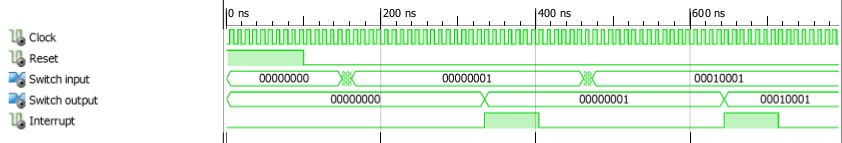
\includegraphics[width=1.0\textwidth]{images/tb6_switch_tb.png}
		\caption{Switch block test bench}
	\end{centering}
\end{figure}
\subsubsection{Conclusion}
The test shows that the interrupt function is working properly, the design is also tested on the Spartan 6 with the LCP2478, and it is working as expected.
% % % % % % % % % % % % % % % % % % % % % % % % % % % % % % % % % % % % % % % % %
% % % % % % % % % % % % % % % % % % % % % % % % % % % % % % % % % % % % % % % % %
% Jesus Thing
% % % % % % % % % % % % % % % % % % % % % % % % % % % % % % % % % % % % % % % % %
\subsection{Web Server - Paulo}
%			Intro
%					verification specification
%					deployment specification
%
In time box 4 a web server was implemented at the ip address 10.1.18.223, this is a virtual machine assign as development environment for the uClinux distribution. The server is running Apache 2, PHP version 5.1.6 and MySQL server 5.0.95.
In this time box a web services system is developed for the communication between the Embedded device and the web server and the other way around. The web page made in Project 3 is incorporated with server side scripts (PHP) for a fully functional web interface.\\
\\An user with read only permissions was created:

User: eval

Pass: ede10eval\\

For evaluation reasons a web application is developed with the name SeeIt, this is a PHP web application that allows the user to see the file structure of the server and the file content, this can be seen at http://10.1.18.223/Seeit/.\\
\\The development of the energy hub web interface can be followed at:

http://e10.ede.hih.au.dk/index.php/Web\_Server\_Structure

The database structure for this project was change to a common database to all modules, the new structure can be seen at:

http://e10.ede.hih.au.dk/index.php/Common\_Database

With the credentials above, the user is able to login into the phpMyAdmin tool in the AU-Herning network at the address: http://10.1.18.223/phpMyAdmin where the database structure is implemented.\\

\subsubsection{Analysis}
%			Analysis
%
%                Refactored block diagram
%                Refactored class diagram
%                Detailed use cases
%                User interface specification
%                System interface specification
%                Dimensioning specification 
%
For a fully functional web interface the communication have to present in both direction, since some teams need to send commands from them web page to the modules.
A file structure was created in the server, where each team have is own folder where all the needed scripts, images and layout styles can be implemented without changing the common layout and requirements approved in project 3.

In this time box the follow scripts are created:
\begin{itemize}
	\item index.php
	\item savedata.php
	\item sendcmd.php
	\item saveip.php
%	\item ajax.js
%	\item login.php
%	\item cron.php
	\item db\_connect.php
	\item db\_globals.php
\end{itemize}

\paragraph{Web interface file Structure}
The file structure is still in development, as such and for the correct version the structure is updated at the address: 

http://e10.ede.hih.au.dk/index.php/Web\_Server\_Structure
%
A short description for each script can be seen bellow:
\begin{itemize}
	\item index.php - First page of the web interface.
	\item savedata.php - Webservice that save data retrieved from the module to the database.
	\item sendcmd.php - Webservice to send commands to the desired module in the system.
	\item saveip.php - Webservice necessary to save the ip address of the energy hub, this will keep the system up and running even if a change on the network is made.
%	\item ajax.js - This Javascript handle AJAX requests when the page have no need to be reloaded, that ensure less bandwidth in the web server.
%	\item login.php  - This PHP script makes the authentication of the user, creating a session when the user gives the right certifications.
%	\item cron.php  - Cron jobs are running by the server in a predefined time, in this case the cron.php at the web server root will point to the cron jobs inside each module folder.
	\item db\_connect.php - Handle the connection to the MySQL database.
	\item db\_globals.php - Includes all the global variables with the credentials for the database.
\end{itemize}

\lineparagraph{Communication}
The server have to save the data retrieved from the system and send commands to the modules connected to the energy hub. Two main scripts are created: \textit{savedata.php} this script capture the values send by the HTTP request has a POST method saving them to the database and \textit{sendcmd.php} enables the user to send commands to a precise module in the system or even the energy hub.
\newpage
Measurements to be saved in the database:
\begin{figure}[H]
	\begin{centering}
		%\missingfigure{Communication savedata.php}
		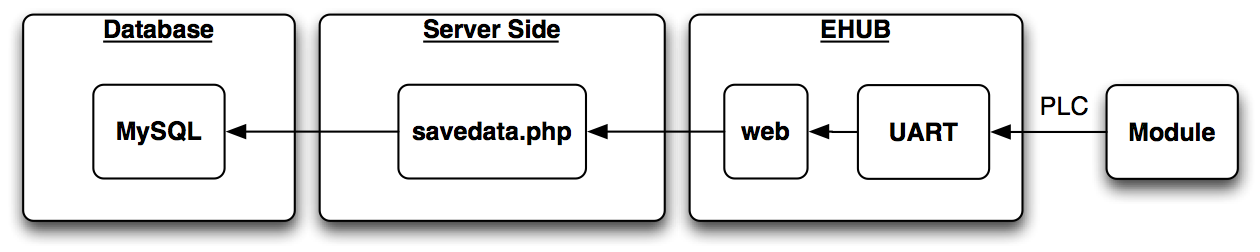
\includegraphics[width=1\textwidth]{images/tb6_webserver_savedata.png}
		\caption{Save measurements retrieved by the modules}
	\end{centering}
\end{figure}
To retrieve the measurements from the modules, an application running at the energy hub translate the data retrieved from the module through PLC to a URL request at the web server. In the server side the web server will collect the data and save it in the database.

Flow of the communication from the user until the final destination in this case the module or the energy hub.
\begin{figure}[H]
	\begin{centering}
		%\missingfigure{Communication SendCmd.php}
		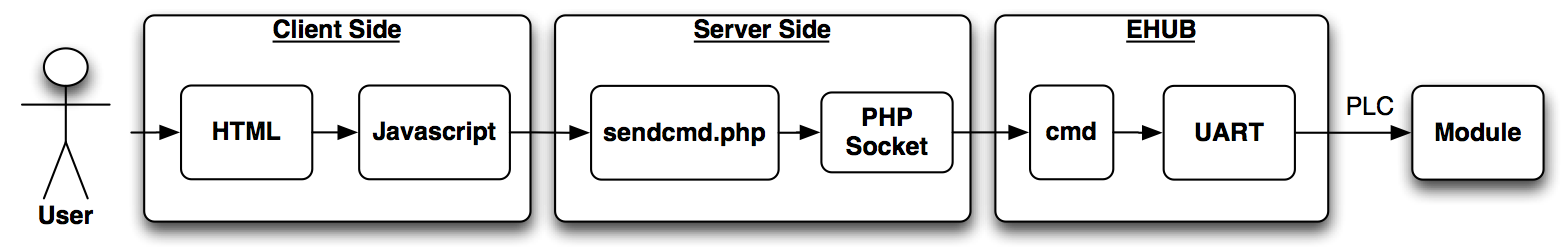
\includegraphics[width=1\textwidth]{images/tb6_webserver_sendcmd.png}
		\caption{Send a command to a module}
	\end{centering}
\end{figure}
This script doesn't give a feedback to the user, the commands send are not verified by the web server or the energy hub. The commands are handle by each module. With this system the flexibility of the system is ensured, since new modules can be added with different functionalities from the already known.
An application running in background at the energy hub OS, ensure that the command is translated to UART so it can be send through the power line communication to the modules.
\\

IP address is send from the Embedded Device:
\begin{figure}[H]
	\begin{centering}
		%\missingfigure{Communication SendCmd.php}
		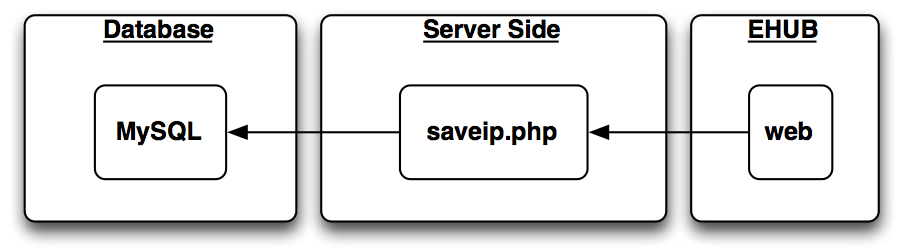
\includegraphics[width=0.8\textwidth]{images/tb6_webserver_saveip.png}
		\caption{Save the IP address of the Embedded device}
	\end{centering}
\end{figure}
A background application running (daemon), ensure that after a reboot, the IP address assigned by DHCP to the energy hub is saved in the database so commands can be send through the web interface. This add flexibility to the system, since a change in the internal network could stop the normal work of the system.

\lineparagraph{Structure Generals}

A folder is created for each team, it will contain the necessary scripts to show data for the users, send commands to the energy hub, make their own layout, etc.

This is a necessary structure for this project, since the requirements are different for all the teams. For example the energy hub page needs to show completely different data from the wind turbine or other modules.

In real production software a general layout and data should be set for all the modules pages, being possible to make small adjustments to satisfy the final user/client. This way the final software would have a improved user experience since the layout is equal in all the modules.

\subsubsection{Design}
%       	 Design
%
%                UML/SysML deployment view(s)
%                Mechanical specifications and dimensioning
%                HW module specification per block
%                UML SW deployment view
%                Class specification
%                Refactored class diagram
%                Use case scenarios specifications
%                Sequence diagrams
The main structure for the correct work of the system is created, in the next time box the energy hub page is built to allow the user to stop and start modules, get the current efficiency as green energy system, etc.

\subsubsection{Implementation}
%     	   Implementation
%
%                Mechanical drawings with details explained
%                Electronic diagrams with details explained
%                Source code with details explained
%                Description of integration 
%
\lineparagraph{index.php}

The \textit{index.php} is the main page of the system, this will redirect the users to the modules or login page.
The efficiency of the system can be seen on the first page as the amount of lamps able to power, the money saved and the mount of less CO2 emissions, this is not available in this version, will be part of the hub web page development in next time box.

\lineparagraph{savedata.php}

A background application running in the energy hub converts the measurement sent through PLC (UART) to a HTTP request \textbf{savedata.php?sensor\_id=ID Sensor\&value=Sensor Measurement\&hub\_port=Hub Port}.

\begin{lstlisting}[language=php]
<?php
	
	require_once("db_connect.php");
	
	$date = getdate();
	
	$today = $date['year'].'-'.$date['mon'].'-'.$date['mday'].' '.$date['hours'].':'.$date['minutes'].':'.$date['seconds'];

	if(isset($_GET['sensor_id']) && isset($_GET['value']) && isset($_GET['hub_port'])){
		$sql= "INSERT INTO `iEnergy`.`MEASUREMENTS` (".
			  "`ID_MEASURE` ,".
			  "`ID_SENSOR` ,".
			  "`DATE_TIME` ,".
			  "`HUB_PORT` ,".
			  "`VALUE`)".
			  "VALUES (NULL , '".$_GET['sensor_id']."', '".$today."', '".$_GET['hub_port']."', '".$_GET['value']."')";
	
		$con->query($sql); // Run the query in the MySQL server
		
		// No feedback needed since the energy hub will not expect an answer.
		
	} else {
		echo 'Incorrect parameters';
	}
	
?>
\end{lstlisting}

This script saves the measurement retrieved from a sensor to the database. At first it established the connection to the MySQL server so SQL requests can be made.
A PHP function returns an array with the current date and time, this is formatted into YYYY-M-D H:M:S, after it can be saved to the MEASUREMENTS table. The script collects all the parameters send through the URL encoding GET, a SQL code is generated and a request made to the MySQL server, the data is added to the MEASUREMENTS table.

\lineparagraph{sendcmd.php}

The web interface is able to send commands to the energy hub and the modules using the\\ \textbf{sendcmd.php?id\_module=\textless module id\textgreater\&cmd=\textless command to be send\textgreater }. The id\_module tells the hub which module the command should be send.
No verification is made of the send command by the web server or the energy hub unless the command is specifically send to the hub.

\begin{lstlisting}[language=php]

	// SQL request for the device page.
	require_once("includes/db_connect.php");
	
	if(isset($_GET['cmd']) && isset($_GET['id_module'])){
	
		$device_port = 5555;
		
		//echo 'Module Id: '.$_GET['id_module']."<BR>Command: ".$_GET['cmd']."<BR>";
		
		$sql= "SELECT IP ". 
			  "FROM `DEVICE` ". 
			  "ORDER BY ID_DEVICE DESC ".
			  "LIMIT 1";
		
		$res = $con->query($sql); // Run the query in the MySQL server
		
		$row = $res->fetch_row();
		
		$device_ip = $row[0];
		
		if ($socket=socket_create(AF_INET, SOCK_STREAM, SOL_TCP)){
			echo "Socket created <br>";
		}
	
		if (socket_connect($socket,$device_ip,$device_port)){
			echo "Connection stablished<br>";	
		} else {
			exit (socket_strerror(socket_last_error()));
		}
	
		$str = $_GET['cmd'].';'.$_GET['id_module'];
		
		socket_write($socket,$str);
	
		socket_close($socket);
		
	} else {
		echo 'Command or Module Id not set';
	}
\end{lstlisting}

At first the script will get the ip address of the energy hub, running a SQL code that retrieves the last IP address added to the table DEVICE. With the energy hub ip and a predefined port, a connection is created using a TCP socket for the communication. The command and the module id are send and the socket is closed.

\lineparagraph{saveip.php}

\textit{saveip.php} script is called by the background application running on the embedded device, it saves the IP address given by DHCP, this is used for further communication between the web server and the energy hub.
\begin{lstlisting}[language=php]
	require_once("includes/db_connect.php");

	if(isset($_GET['ip'])){
		$sql= "INSERT INTO `iEnergy`.`DEVICE` (".
			  "`ID_DEVICE` ,".
		  	  "`IP`)".
		  	  "VALUES (NULL , '".$_GET['ip']."')";
	
		$con->query($sql); // Run the query in the MySQL server
		
		// No feedback needed since the energy hub will not expect an answer.
		
	} else {
		echo 'IP not set';
	}
\end{lstlisting}
The ip address is send by the GET method (saveip.php?ip=127.0.0.1), this is how the data in encoded into a URL, being collected in the variable \$\_GET['ip']. 
A \$sql variable string is created containing the SQL code to be run at the MySQL server.

\lineparagraph{db\_connect.php}

For the communication to the database a driver is used in PHP that provides an interface to the MySQL server. The PHP mysqli extension (MySQL improved) is used in this project, this is recommend for MySQL servers version 4.1.3 or later. This extension provides several benefits as a objective-oriented interface, support for multiple statements, embedded server support and more can be found in the MySQL documentation.

\begin{lstlisting}[language=php]
	require_once("db_globals.php");
	
	$con = new mysqli(DB_HOST,DB_USER,DB_PASS,DB_NAME); // Creates new mysql connection
	
	if($con->connect_error){
		echo "Failed to connect to MySQL: (" . $con->connect_errno . " ) ". $con->connect_error;
	} 
	else { echo "Connection established"; }
\end{lstlisting}

In this script an object is instantiated with a connection to the MySQL server.

\textit{\$con = new mysqli\textless parameters \textgreater)}

The parameters are included from the db\_globals.php, setting the server host, user, password and database to be used.

\lineparagraph{db\_globals.php}

Using a script to define the parameters for the MySQL connection, 
All the scripts that need to use the global parameters for the connection to the MySQL server, should include db\_globals.php as shown in the db\_connect.php above.

\begin{lstlisting}[language=php]
	// MySQL condifuration
	DEFINE ('DB_USER','root');
	DEFINE ('DB_PASS','root');
	DEFINE ('DB_HOST','localhost');
	DEFINE ('DB_NAME','iEnergy');
\end{lstlisting}

The global parameters the connection to the MySQL server are define in this script.

\begin{itemize}
	\item DB\_USER - Database user name with read, write and execute permissions.
	\item DB\_PASS - Password for the user
	\item DB\_HOST - Hostname for the MySQL server, if running at the same host as the PHP server, localhost or 127.0.0.1 should be used.
	\item DB\_NAME - Database name to connect to.
\end{itemize}

\subsubsection{Verification}
%       	 Verification
%
%                Module tests
%                Integration tests
%                Acceptance test
The verification is made using the tools described in the beginning of this section:
\begin{table}[H]
\centering
	\begin{tabular}{| c | l | c |}
		\hline
		Verification & Description & Acceptance \\\hline
		1 & Save new IP address: saveip.php?ip=127.0.0.1 & OK \\\hline
		2 & Send command: sendcmd.php?unique\_id=0\&cmd=led 1 on & TimeBox7 \\\hline
		3 & File structure created & OK \\\hline
	\end{tabular}
\end{table}

\subsubsection{Conclusion}
The common web services and file structure in the web server was created for all the modules/teams.\\
The implementation of the savedata.php will required further analysis for a working system, since the energy hub needs to have a table of all the sensors connected to each module. When a module retrieves a value the hub needs to know which sensor the measurement belongs to. This was not taken in consideration in earlier analysis of the system and might affect the protocol developed and system dynamics.\\
In the next time box a scaled down prototype is developed and the communication dynamics between web server and modules can be tested.

% % % % % % % % % % % % % % % % % % % % % % % % % % % % % % % % % % % % % % % % %
% % % % % % % % % % % % % % % % % % % % % % % % % % % % % % % % % % % % % % % % %
% Dennis Thing
% % % % % % % % % % % % % % % % % % % % % % % % % % % % % % % % % % % % % % % % %
\subsection{UART Device driver improvements - Dennis}
As described in section \ref{sec:device_driver_conclusion}, some improvements should be implemented in order to boost performance on the UART devices. The parts which will be further implemented in the UART device driver is:
\begin{itemize}
	\item Interrupt controlled read.
	\item More flexibel initialization. 
	\item Better feedback/help description to the user. 
\end{itemize}
Furthermore it was pointed out (by Klaus Kolle) that the implemented way of setting up the device broke general politic for device drivers. To avoid this, an IOCTL (Input Output Control) function shall be implemented to take care of all setup and to leave the write function to sending characters. 
%			Intro
%					verification specification
%					deployment specification
%
%\subsubsection{Analysis}
%			Analysis
%
%                Refactored block diagram
%                Refactored class diagram
%                Detailed use cases
%                User interface specification
%                System interface specification
%                Dimensioning specification 
%
\subsubsection{Design}
The functionalities implemented in the IOCTL call are:
\begin{itemize}
	\item Help command. Write out the different choices of IOCTL calls.
	\item Default setup call. Sets up the defined UART to 8n1, 9600 baud rate. 
	\item Baud rate. Set a baud rate in the range 2400 to 230400.
	\item Word length. Define the word length between 5 and 8.
	\item Stop bits. Number of stop bits, 1 or 2.
	\item Parity bits. Define parity bit setting: none, odd, even, forced 1 stick, forced 0 stick.
	\item Fifo. Enable or disable fifo.
	\item Fifo trigger. Number of characters in the buffer before an interrupt: 1,4,8,14
\end{itemize}

%       	 Design
%
%                UML/SysML deployment view(s)
%                Mechanical specifications and dimensioning
%                HW module specification per block
%                UML SW deployment view
%                Class specification
%                Refactored class diagram
%                Use case scenarios specifications
%                Sequence diagrams
%
\subsubsection{Implementation}
Common header file for the UART device driver and the UART user space application. The magic number 'k' is used to by the IOCTL macros \_IO and \_IOR to create an IOCTL number, which is then decoded and verified in the kernel module. 
\begin{lstlisting}[language=c]
#ifndef UARTIOCTL_H
#define UARTIOCTL_H

#include <linux/ioctl.h>

#define UART_IOC_MAGIC  'K'

#define IOCTL_HELP 		_IO(UART_IOC_MAGIC,  1)
#define IOCTL_DEFAULT	_IO(UART_IOC_MAGIC,  2)
#define IOCTL_BAUD 		_IOR(UART_IOC_MAGIC, 3, int)
#define IOCTL_WORDLEN 	_IOR(UART_IOC_MAGIC, 4, int)
#define IOCTL_STOPBIT 		_IOR(UART_IOC_MAGIC, 5, int)
#define IOCTL_PARBIT 		_IOR(UART_IOC_MAGIC, 6, int)
#define IOCTL_FIFO			_IOR(UART_IOC_MAGIC, 7, int)
#define IOCTL_FIFO_TRIG 	_IOR(UART_IOC_MAGIC, 8, int)

#define UART_IOC_MAXNR 8

#endif
\end{lstlisting}

Using IOCTL to setup UART registers. Note that the \textit{fwrite} call cannot be used with IOTCL, as it needs an file descriptor instead of a file pointer. Therefore the libraries \textit{fcntl.h} and \textit{unistd.h} are included in order to use the functions \textit{open, close, read, write} and \textit{ioctl} as they make use of the file descriptor. 
\begin{lstlisting}[language=c]
	if(strncmp("io", argv[1], 2) == 0){
		if ((fd = open(UART,O_RDWR)) < 0){
     	          	printf("Cannot open file.\n");
			exit(-1);
        	}

		ret_val = ioctl(fd, IOCTL_DEFAULT);
		if(ret_val < 0){
			printf("ioctl_get_msg failed:%d\n", ret_val);
			exit(-1);
		}
		ret_val = ioctl(fd, IOCTL_BAUD, 19200);
		if(ret_val < 0){
			printf("ioctl_get_msg failed:%d\n", ret_val);
			exit(-1);
		}

		close(fd);
	}
\end{lstlisting}
Loop reading used for testing purpose of the power line communication. 
\begin{lstlisting}[language=c]
	---
	else if(strncmp("readloop", argv[1], 8) == 0){
		if ((fd = open(UART,O_RDONLY)) < 0){		//Open the file
     	          	printf("Cannot open file.\n");
			exit(-1);
        	}
		while(1){
			if(read(fd,rb,10) != 0) 
				printf("%s\n",rb);
		}
		printf("\n");
		close(fd);
	}
\end{lstlisting}

IOCTL added to file operator
\begin{lstlisting}[language=c]
static struct file_operations uart_fops = {
	.owner   	= THIS_MODULE,
	.read			= uart_read,
	.write  	= uart_write,
	.open    	= uart_open,
	.ioctl	 	= uart_ioctl,
	.release 	= uart_close,
};
\end{lstlisting}

IOCTL implementation. At first the function verifies the IOCTL number sent and checks if the transferred command is valid. The rest of the function is a  switch/case which takes the cmd parameter sent and performs an action according to the command (help, default setup, baud rate etc.)
\begin{lstlisting}[language=c]
/******************************************************************************
 * IOCTL call
 *****************************************************************************/
static int uart_ioctl(struct inode *inode, struct file *filp, unsigned int cmd, unsigned long arg){
	unsigned int num = 0;
        int err = 0, ret = 0;
	int div, mult,bflag = 0;
	unsigned int baud = 0;

        /* don't even decode wrong cmds: better returning  ENOTTY than EFAULT */
        if (_IOC_TYPE(cmd) != UART_IOC_MAGIC) return -ENOTTY;
        if (_IOC_NR(cmd) > UART_IOC_MAXNR) return -ENOTTY;

        /*
         * the type is a bitmask, and VERIFY_WRITE catches R/W
         * transfers. Note that the type is user-oriented, while
         * verify_area is kernel-oriented, so the concept of "read" and
         * "write" is reversed
         */
        if (_IOC_DIR(cmd) & _IOC_READ) err = !access_ok(VERIFY_WRITE, (void __user *)arg, _IOC_SIZE(cmd));
        else if (_IOC_DIR(cmd) & _IOC_WRITE) err =  !access_ok(VERIFY_READ, (void __user *)arg, _IOC_SIZE(cmd));
        if (err) return -EFAULT;
	// Get minor number
	num = MINOR(inode->i_rdev);
	DPRINT("\nuart%d_ioctl, ioctl_cmd: %u\n",num,cmd);
	// Check if minor number is okay
	if(num >= NUM_UART_DEVICES){
		return -ENODEV;
	}

	switch (cmd) {
	/***************************** HELP ************************************************/
	case IOCTL_HELP:
	    DPRINT("\nHELP\n");
	    help();	// Print different IOCTL call options to user
	  break;
	/***************************** DEFAULT *********************************************/
	case IOCTL_DEFAULT:
	    m_reg_write(ulcr[num], 0x80);	// Enable write to divisor latch
	    m_reg_write(udll[num], (unsigned char)((LPC24xx_Fpclk/(16*9600)) & 0xFF));
	    m_reg_write(udlm[num], (unsigned char)((LPC24xx_Fpclk/(16*9600)) >> 8));
	    m_reg_write(ulcr[num], 0x03);	// 8N1 setup and disable write to divisor latch
	    m_reg_write(ufcr[num], 0x7);	// Enable FIFO's
	  break;
	/***************************** BAUD ************************************************/
	case IOCTL_BAUD:
	    if(arg < 2400 || arg > 230400){	// Verify argument
		printk("\nInvalid parameter");
		return -EFAULT;
	    }
	    bflag = 0;	
	/* From datasheet:
	   Mult values: 1-15, Div: 0-14. Mult shall be bigger than div.
	   DLL shall be above 2 if DLM is zero.

	*/ 
	   // Loop through different div and mult values in order to get a integer value to
	   // the divisor latch reg (DLM+DLL).
	    for(div = 0; div <= 15; div++){
		for(mult = div+1; mult <= 15; mult++){
		    baud = ((16*arg)+((16*arg*div)/mult));
		    if(LPC24xx_Fpclk%baud == 0){
			if((div != 0) && ((LPC24xx_Fpclk/baud) >= 3)){
			    bflag = 1;
			    break;
			}
		    }
		}
		if(bflag==1) break;
	    }
	    DPRINT("\ndiv: %d, mult: %d, baud: %d",div,mult,baud);
	    if(div == 15){	// If no value was found, return error
		printk("\nCannot calculate BAUD!");
		return -EFAULT;
	    }
	    m_reg_bfs(ulcr[num], 0x80); // Enable write to divisor latch
	    m_reg_write(ufdr[num], ((div<<0) | (mult<<4)));	// Write div and mult to fraction dividor reg
	    m_reg_write(udll[num], (unsigned char)((LPC24xx_Fpclk/baud) & 0xFF)); // Input DLL val (8 lowest bits)
	    m_reg_write(udlm[num], (unsigned char)((LPC24xx_Fpclk/baud) >> 8));	  // Input DLM val (8 highest bits)
	    m_reg_bfc(ulcr[num], 0x80);	// Disable write to divisor latch

	  break;
	/***************************** Wordlen *********************************************/
	case IOCTL_WORDLEN:
	    if(arg < 5 || arg > 8){	// Verify that argument is valid
		printk("\nInvalid parameter");
		return -EFAULT;
	    }
	    m_reg_bfc(ulcr[num], 0x3);	// Clear bits holding world lenght
	    m_reg_bfs(ulcr[num], ((arg-5)<<0));	// Inset value for world lenght
	  break;
	/***************************** STOP bits *******************************************/
	case IOCTL_STOPBIT:
	    if(arg != 1 || arg != 2){	// Verify that argument is valid
		printk("\nInvalid parameter");
		return -EFAULT;
	    }
	    m_reg_bfc(ulcr[num], (1<<2)); // Set stop bit to 1
	    if(arg == 2){
	    	m_reg_bfs(ulcr[num], (1<<2)); // Set stop bit to 2
	    }
	  break;
	/***************************** Parity Bit ******************************************/
	case IOCTL_PARBIT:	
	    if(arg < 0 || arg > 4){ // Verify that argument is valid
		printk("\nInvalid parameter");
		return -EFAULT;
	    }
	    m_reg_bfc(ulcr[num], (1<<3));	// Disable parity bits. if 0 was written
	    if(arg > 0){
		m_reg_bfs(ulcr[num], (1<<3));	// Enable parity.
		m_reg_bfs(ulcr[num], ((arg-1)<<4)); // Set parity (odd, even, forced 0 or 1
	    }
	  break;
	/***************************** FIFO Enable *****************************************/
	case IOCTL_FIFO:
	    if(arg != 0 || arg != 1){ // Verify that argument is valid
		printk("\nInvalid parameter");
		return -EFAULT;
	    }
	    m_reg_bfc(ufcr[num], 0x7);	// Disable fifo
	    if(arg==1){
		m_reg_bfs(ufcr[num], 0x7);	// Enable fifo
	    }
	  break;	
	/***************************** FIFO Enable *****************************************/
	case IOCTL_FIFO_TRIG:
	    if(arg != 1 || arg != 4 || arg != 8 || arg != 14){	// Verify that argyment is valid
		printk("\nInvalid parameter");
		return -EFAULT;
	    }
	    m_reg_bfc(ufcr[num], 0xC0);	// Clear bits holding trigger level
	    m_reg_bfs(ufcr[num], (int)((arg/4)<<6));	// 1/4=0, 4/4=1, 8/4=2, 14/4=3
	  break;	
	/***************************** Wrong ***********************************************/
	default:
	    help();	// If wrong parameter sent. Print options. 
	    return -ENOTTY;
	}

        return ret;
}
\end{lstlisting}

Interrupt implementation. The interrupt is requested in the open call. If there is no data to read, the module is sent to sleep and awaken again when the buffer is not empty anymore. In close the interrupt is freed again. 
\begin{lstlisting}[language=c]
//Interrupt sources for UART0,1,2,3
#define UART0_IRQ 6 
#define UART1_IRQ 7
#define UART2_IRQ 28
#define UART3_IRQ 29
//Array of interrupt flags
static int flag[NUM_UART_DEVICES];

//Prototypes of interrupt functions. Int\_uart is an array of function pointers.
static irqreturn_t interrupt_uart0(int irq, void *dev_id);
static irqreturn_t interrupt_uart1(int irq, void *dev_id);
static irqreturn_t interrupt_uart2(int irq, void *dev_id);
static irqreturn_t interrupt_uart3(int irq, void *dev_id);
typedef irqreturn_t (*INTERRUPT_UART)(int irq, void *dev_id);
const INTERRUPT_UART int_uart[NUM_UART_DEVICES] = {interrupt_uart0, interrupt_uart1, interrupt_uart2, interrupt_uart3};

static int uart_open(struct inode* inode, struct file* file){
---
	flag[num] = 0;
	m_reg_write(uier[num], 0x1);	//Enable interrupt on rx buf not empty
	m_reg_bfs(VICSoftIntClear, (1<<uirq[num])); // Clear interrupts from uart source
	m_reg_bfs(VICIntEnable, (1<<uirq[num]));    // Enable uart interrupt

	ret = request_irq(uirq[num], int_uart[num], SA_INTERRUPT,"UART interrupt", NULL); //NULL = Pointer based on IRC handler

	if(ret){
		printk("IRQ %d is not free. RET: %d\n", UART2_IRQ,ret);
		return ret;
	}
	return 0;
}

static int uart_close(struct inode* inode, struct file* file){
	---
	free_irq(uirq[num], NULL);	// Free interrupt
	return 0;
}
\end{lstlisting}
UART read call.
\begin{lstlisting}[language=c]
static ssize_t uart_read(struct file *p_file, char *p_buf, size_t count, loff_t *p_pos){
	---
	if(!(m_reg_read(ulsr[num]) & 0x01)){		//If the read buffer is empty, go to sleep.
		DPRINT("\nBUF EMPT, SLEEP\n");
		wait_event_interruptible(my_queue, (flag[num] != 0));	// Put the function to sleep
		flag[num] = 0;
	}
	else{
		cread = m_reg_read(urbr[2]);
	}
	*p_buf = cread;		// Write value to read buffer. 
	
	return count;
}
\end{lstlisting}
UART interrupt function. The four different interrupt functions are all similar, except for the registers that is handled. 
\begin{lstlisting}[language=c]
/******************************************************************************
 * Interrupt recieve routine UART2
 *****************************************************************************/
static irqreturn_t interrupt_uart2(int irq, void *dev_id){
	
	cread = m_reg_read(urbr[2]);		// Read the buffer
	
	DPRINT("\nREAD VAL: %c\n", cread);		

	m_reg_bfs(VICSoftIntClear, (1<<uirq[2]));		// Clear int flag in vic
	flag[2] = 1;	
	wake_up_interruptible(&my_queue);		// Wake up from interrupt
	return IRQ_HANDLED;
}
\end{lstlisting}

The help function implemented gives the following input if it is called:
\begin{lstlisting}[language=c]
# ./uart help
Available commands:
  IOCTL_HELP : show different help commands
  IOCTL_DEFAULT : 8N1, 9600 baud
  IOCTL_BAUD : send argument between 2400 and 230400
  IOCTL_WORDLEN : send argument 5-8 wordlenght
  IOCTL_STOPBIT : send argument, 1 or 2 stop bits
  IOCTL_PARBIT : send arg, 0, 1(odd), 2(even), 3(Forced 1 stick), 4(Forced 0 stick
  IOCTL_FIFO : send arg 0 (off), 1 (on)
  IOCTL_FIFO_TRIG : send arg number to trig, 1, 4, 8 or 14 characters
\end{lstlisting}

\subsubsection{Verification}
According to the requirement F-1.2 and the test for it, the communication between two modules have been tested over power line. 
\begin{table}[H]
\centering
	\begin{tabular}{|p{1.2cm}|p{2.3cm}|p{9.5cm}|p{2.5cm}|}
	\hline
	ID		& Requirement		& Test Description		& Grade/Comment\\\hline
	F-1.2		& Communication - System & Connect a module to the hub, by connecting the module to the hubs power line (plugs on the back of the hub). If the module respond to a ping signal send from the hub, the two modules are communicating through power line. The response of the ping can be seen by using an oscilloscope and simply analyzing the packages on the power line according to the protocol. & PASSED\\\hline
	\end{tabular}
\end{table}
A small test setup have been made with a MBED device as one of the modules and an ARM board running uClinux as the other module. Data have been sent in both direction (from the MBED to the ARM and from the ARM to the MBED) through each of their Power Line modules, with use of the UART user space application written. The default settings of the Power Line module is 8N1 with a baud rate of 19200 which has been used for the test. 
\\ The test has passed. No invalid or missing data have been observed throughout the test. 
%       	 Verification
%
%                Module tests
%                Integration tests
%                Acceptance test
\subsubsection{Conclusion}
The UART module is working with implemented IOCTL and interrupt handler.
Further improvements before the fully functional energy system can use the UART driver is implementation of file write.
% % % % % % % % % % % % % % % % % % % % % % % % % % % % % % % % % % % % % % % % %
% % % % % % % % % % % % % % % % % % % % % % % % % % % % % % % % % % % % % % % % %
% Deployment
% % % % % % % % % % % % % % % % % % % % % % % % % % % % % % % % % % % % % % % % %
\subsection{Deployment}
	%which versions of the prototype the customer will get
	%with what functionality.
\paragraph{Switch interrupt}
The switch block is the last part in the Spartan 6. The VHDL coding for the Spartan 6 is finished, the last part is to test it all together and verify that everything works.
%
%
\paragraph{Web Server}
The web server is up and running with the basic structure for the web interface development. The web server is able to send commands to the energy hub and it will route the commands to the desired module. For a complete system the applications running in background will be developed so all the communication can be handle.
%
%
\paragraph{UART Device driver improvements}
The UART device driver is working with implemented interrupt handling, input output control and clean write function. Klaus Kolle and Morten Opprud have been by and verified the test setup. 
%
%\newpage
%% % % % % % % % % % % % % % % % % % % % % % % % % % % % % % % % % % % % % % % % %
% INTRO
% % % % % % % % % % % % % % % % % % % % % % % % % % % % % % % % % % % % % % % % %
\section{Time box 7}
\listoftodos
\subsection{Time box planning}

\begin{figure}[H]
	\begin{centering}
		\missingfigure{Updated timebox figure}
		%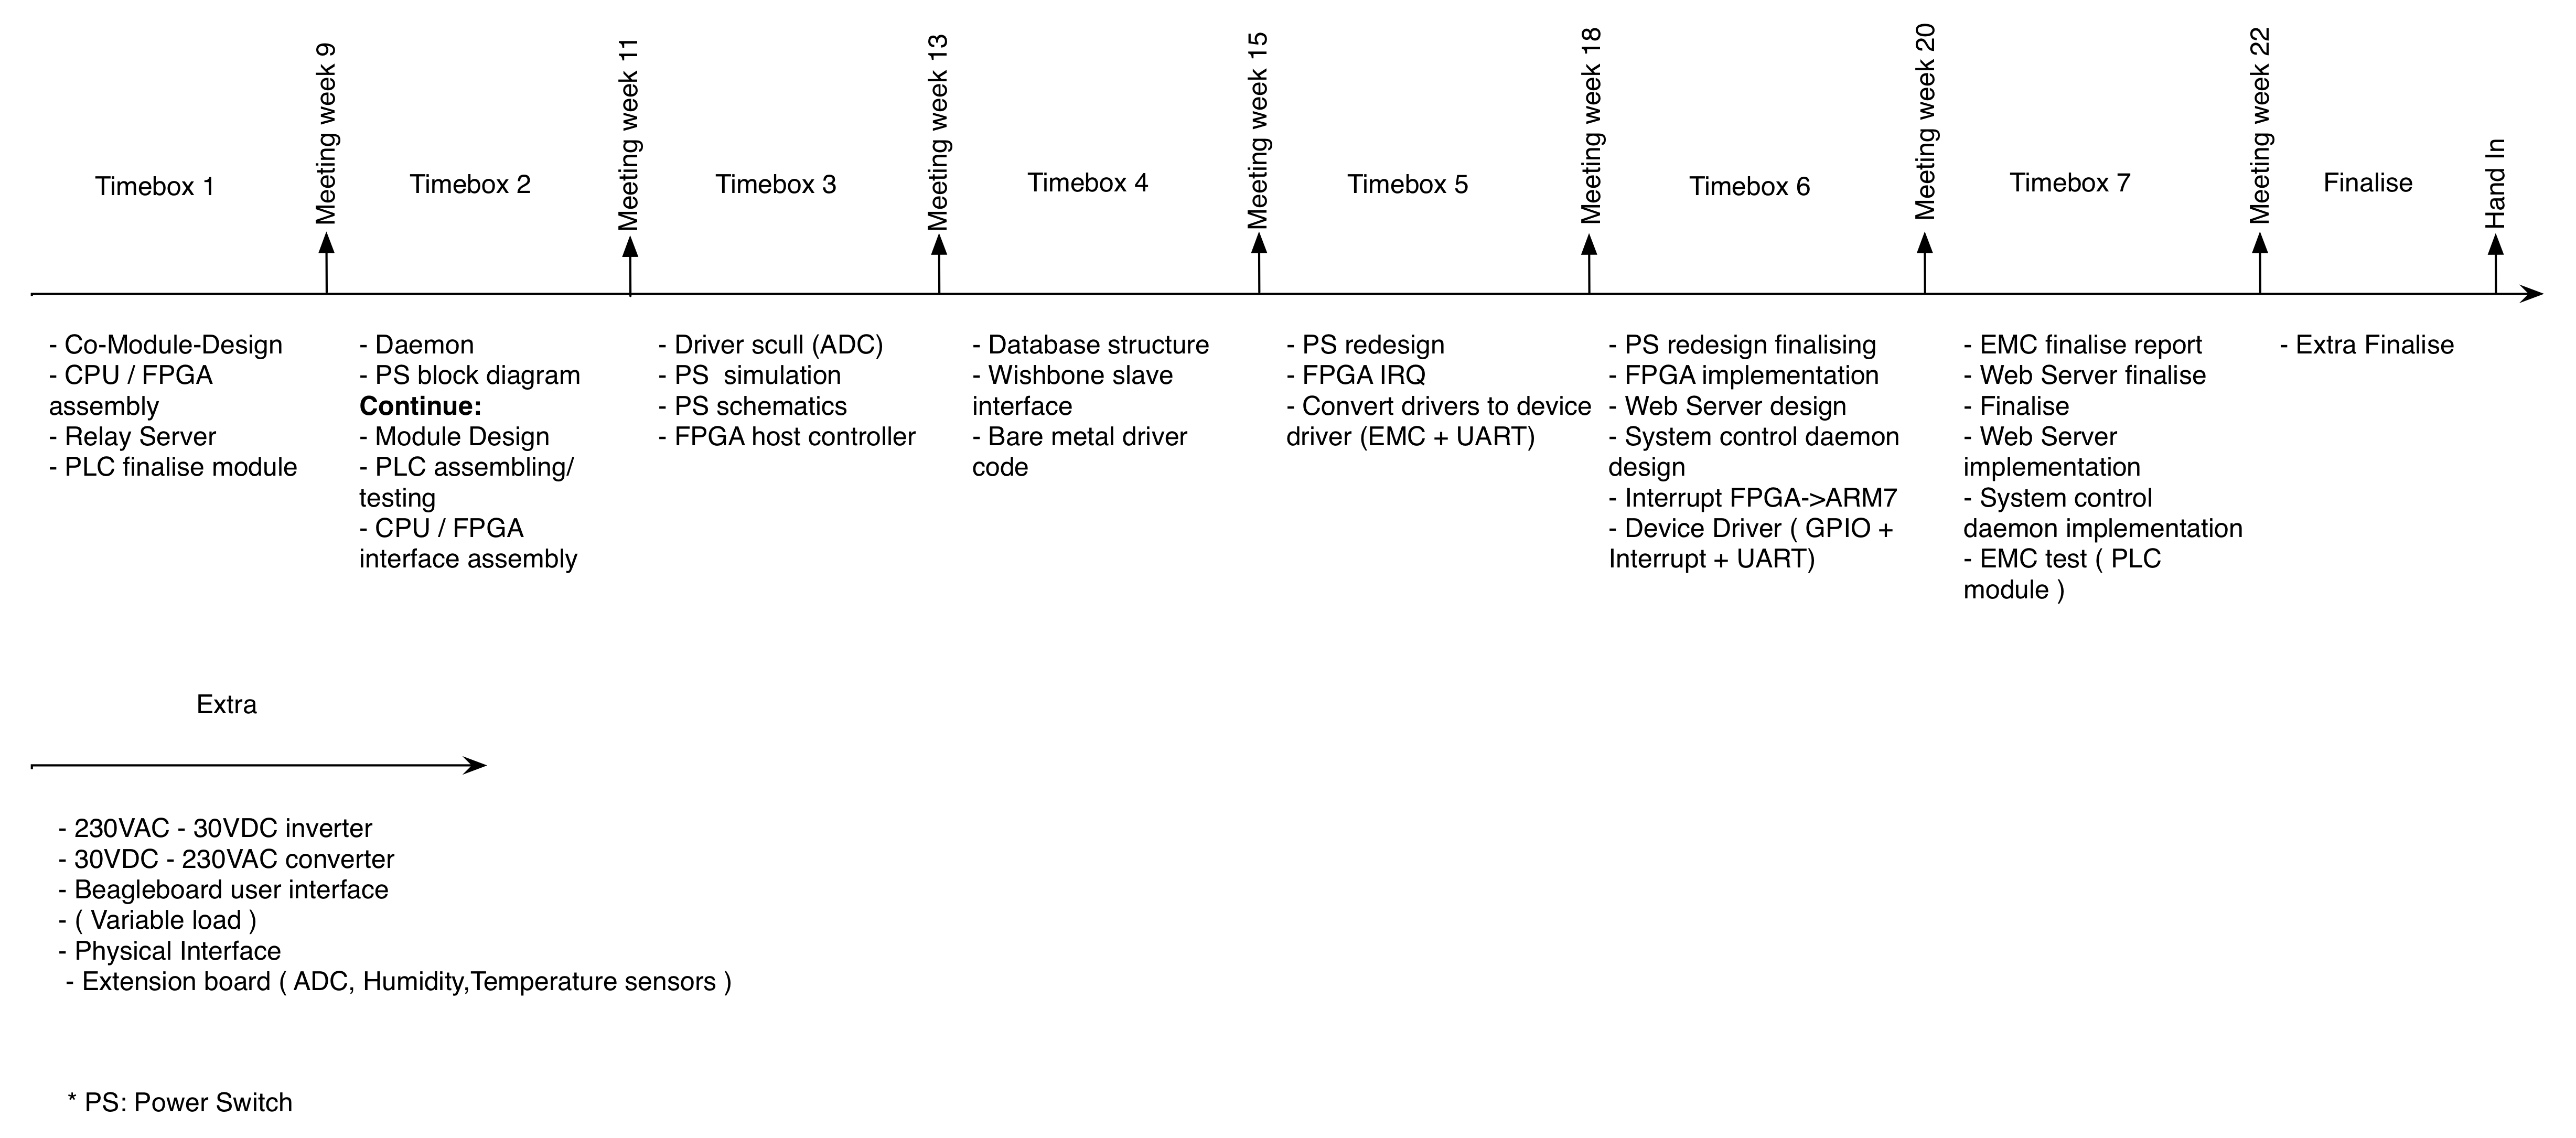
\includegraphics[width=1.0\textwidth]{images/tb_r5.png}
		%\caption{Updated time-box}
	\end{centering}
\end{figure}

\subsubsection{Work to be done in this time box}
\todo[inline]{Update List}
\begin{itemize}
	\item Theis thing
	\begin{itemize}
		\item Sub thing
	\end{itemize}
	\item Jesus thing
		\begin{itemize}
			\item sub thing
		\end{itemize}
	\item Dennis thing
	\begin{itemize}
		\item Sub thing
	\end{itemize}
\end{itemize}

\paragraph{Description:}
\todo[inline]{Update Description}
\begin{description}
	\item[Theis thing]
	\item[Jesus thing]
	\item[Dennis thing]
\end{description}

\subsubsection{Time planning}

\begin{table}[H]
\centering
	\todo[inline]{Update Time}
	\begin{tabular}{|l|c|c|c|c|c|}
		\hline
		~			& Theis thing			& Jesus thing		& Dennis thing	\\ \hline
		Estimation	& xx					& xx				& xx			\\
		Actual		& xx					& xx				& xx			\\
		Developer	& Theis					& Paulo				& Dennis		\\
		\hline
	\end{tabular}
	\caption{Estimation and actual time used on the project}
\end{table}
% % % % % % % % % % % % % % % % % % % % % % % % % % % % % % % % % % % % % % % % %
% % % % % % % % % % % % % % % % % % % % % % % % % % % % % % % % % % % % % % % % %
% Theis Thing
% % % % % % % % % % % % % % % % % % % % % % % % % % % % % % % % % % % % % % % % %
\subsection{Theis thing - Theis}
%			Intro
%					verification specification
%					deployment specification
%
\subsubsection{Analysis}
%			Analysis
%
%                Refactored block diagram
%                Refactored class diagram
%                Detailed use cases
%                User interface specification
%                System interface specification
%                Dimensioning specification 
%
\subsubsection{Design}
%       	 Design
%
%                UML/SysML deployment view(s)
%                Mechanical specifications and dimensioning
%                HW module specification per block
%                UML SW deployment view
%                Class specification
%                Refactored class diagram
%                Use case scenarios specifications
%                Sequence diagrams
%
\subsubsection{Implementation}
%     	   Implementation
%
%                Mechanical drawings with details explained
%                Electronic diagrams with details explained
%                Source code with details explained
%                Description of integration 
%
\subsubsection{Verification}
%       	 Verification
%
%                Module tests
%                Integration tests
%                Acceptance test
\subsubsection{Conclusion}
% % % % % % % % % % % % % % % % % % % % % % % % % % % % % % % % % % % % % % % % %
% % % % % % % % % % % % % % % % % % % % % % % % % % % % % % % % % % % % % % % % %
% Jesus Thing
% % % % % % % % % % % % % % % % % % % % % % % % % % % % % % % % % % % % % % % % %
\subsection{Jesus thing - Paulo}
%			Intro
%					verification specification
%					deployment specification
%
\subsubsection{Analysis}
%			Analysis
%
%                Refactored block diagram
%                Refactored class diagram
%                Detailed use cases
%                User interface specification
%                System interface specification
%                Dimensioning specification 
%
\subsubsection{Design}
%       	 Design
%
%                UML/SysML deployment view(s)
%                Mechanical specifications and dimensioning
%                HW module specification per block
%                UML SW deployment view
%                Class specification
%                Refactored class diagram
%                Use case scenarios specifications
%                Sequence diagrams
%
\subsubsection{Implementation}
%     	   Implementation
%
%                Mechanical drawings with details explained
%                Electronic diagrams with details explained
%                Source code with details explained
%                Description of integration 
%
\subsubsection{Verification}
%       	 Verification
%
%                Module tests
%                Integration tests
%                Acceptance test
\subsubsection{Conclusion}
% % % % % % % % % % % % % % % % % % % % % % % % % % % % % % % % % % % % % % % % %
% % % % % % % % % % % % % % % % % % % % % % % % % % % % % % % % % % % % % % % % %
% Dennis Thing
% % % % % % % % % % % % % % % % % % % % % % % % % % % % % % % % % % % % % % % % %
\subsection{Dennis thing - Dennis}
%			Intro
%					verification specification
%					deployment specification
%
\subsubsection{Analysis}
%			Analysis
%
%                Refactored block diagram
%                Refactored class diagram
%                Detailed use cases
%                User interface specification
%                System interface specification
%                Dimensioning specification 
%
\subsubsection{Design}
%       	 Design
%
%                UML/SysML deployment view(s)
%                Mechanical specifications and dimensioning
%                HW module specification per block
%                UML SW deployment view
%                Class specification
%                Refactored class diagram
%                Use case scenarios specifications
%                Sequence diagrams
%
\subsubsection{Implementation}
%     	   Implementation
%
%                Mechanical drawings with details explained
%                Electronic diagrams with details explained
%                Source code with details explained
%                Description of integration 
%
\subsubsection{Verification}
%       	 Verification
%
%                Module tests
%                Integration tests
%                Acceptance test
\subsubsection{Conclusion}
% % % % % % % % % % % % % % % % % % % % % % % % % % % % % % % % % % % % % % % % %
% % % % % % % % % % % % % % % % % % % % % % % % % % % % % % % % % % % % % % % % %
% Deployment
% % % % % % % % % % % % % % % % % % % % % % % % % % % % % % % % % % % % % % % % %
\subsection{Deployment}
	%which versions of the prototype the customer will get
	%with what functionality.
\paragraph{Theis thing}
%
%
\paragraph{Jesus thing}
%
%
\paragraph{Dennis thing}
%
%\newpage
%\section{Time box}
Things that cannot be done before week 21.
\begin{itemize}
	\item 230VAC-> 30DVC converter
	\item 30VDC -> 230VAC converter
	\item Variable load
	\item BeagleBoard running for local client of website (User interface)
\end{itemize}